\chapter{Implementation}

In this chapter we will outline the program structure. We will
demonstrate the flexibility as well as the limitations of our
implementation.


%%%%%%%%%%%%%%%%%%%%%%%%%%%%%%%%%%%%%%%%%%%%%%%%%%%%%%%%%%%%%%%%%%%%
%                                                                  %
%                      Structure of the QMC Program                %
%                                                                  %
%%%%%%%%%%%%%%%%%%%%%%%%%%%%%%%%%%%%%%%%%% %%%%%%%%%%%%%%%%%%%%%%%%%
\section{Structure the QMC Program}


%%%%%%%%%%%%%%%%%%%%  Programming Philosophy  %%%%%%%%%%%%%%%%%%%%%%
\subsection{Programming Philosophy}

There are three major concepts concerning the implementation of any
large program:

\begin{enumerate}
  \item{} Speed - the computational time (CPU).
  \item{} Flexibility - ability to handle many different special cases.
  \item{} Readability - how easy it is to understand the program (and
  make modifications).
\end{enumerate}

In order to include flexibility, the
program should consist of many small building blocks, that may easily
be replaced by other similar blocks. The program structure should also
be legible. Often, modifications of existing programs need to be done,
either by the programmers themselves, or by other users. This task may
be very time consuming, especially if the program is difficult to
understand. The algorithms and data structure 
need to be well documented, the building blocks\footnote{Classes
  in C++, modules in Fortan90/50 etc.} should seem like natural
choices, and the variables names should be meaningful. \newline

Futhermore, programs may run for days on powerful machines in order to
accuire the desired result. Therefore, a great deal of effort must be
put into the design and development of the program. \newline


%%%%%%%%%%%%%%%%%%%% Main Program Structure %%%%%%%%%%%%%%%%%%%%%%%
\subsection{Main Program}

Our first concern is to recognice what the program is going to do, and
to form a program stucture. We divide the program into blocks, that
each preform some specific task. Figure \ref{program_stucture} illustrates
the basic structure of our main program. 

\begin{figure}[hbtp]
\begin{center}
  \epsfig{file=Implementation/program.eps, height=8cm}
  \caption{Variational Monte-Carlo program structure}
  \label{program_stucture}
\end{center}
\end{figure}

Generally, the user must provide some input to specify what the
computer is going to calculate.  After the input is specified, the
user does not need to do anything until the program is terminated. The
output should be presented in an easy and orderly fashion; either at
the end of the program execution, or by user specifications after the
run is completed. \newline

Dependent of the user input, the program will execute one or more runs
of the VMC algorithm. The program loops different configurations and
parameter settings, in order to localize an energy (or variance)
minimum. Each setting generate the input, the \emph{initial setup},
for a VMC calulation, and for each VMC run the program genrates an
\emph{output}. Typically, this output is for user deguging. For
example, if the initial parameter input is off bounds (and the program
terminates without finding an energy minimum) the user may chech these
outputs to adjust the user specified input for another run.


%%%%%%%%%%%%%%%%%%%%%%%%% Input Structure %%%%%%%%%%%%%%%%%%%%%%%%%
\subsection{Input}

The input structure is given by figure \ref{input_stucture}.

\begin{figure}[hbtp]
\begin{center}
  \epsfig{file=Implementation/input.eps, height=5.7cm}
  \caption{Input structure}
  \label{input_stucture}
\end{center}
\end{figure}

The user must specify the atom to be studied, and what state is to be
found - e.g. the He 2$^{nd}$ excited $^1S_0$-state. The trial wavefunction
must also be specified, both the variational form of the orbital
wavefuntions and of the Jastrow-factor. These choices gives raise to a
set of parameters, and the user must provide some inital guess, and
tell wich parameters is to be varied. The user must further set some
termination criteria, TC, for example number of Monte-Carlo
cycles. Some other parameters must also be set, either by the program,
or by the user; number of dimensions, output file-name(s), etc.


%%%%%%%%%%%%%%%% Loop Parameters & Configurations %%%%%%%%%%%%%%%%%
\subsection{Loop Parameters \& Configurations}

Figure \ref{loop_parameters_config} outlines the \emph{loop parameters \&
configurations} structure.

\begin{figure}[hbtp]
\begin{center}
  \epsfig{file=Implementation/loop_parameters_config.eps, height=7cm}
  \caption{Structure of parameter and configuration loop}
  \label{loop_parameters_config}
\end{center}
\end{figure}

We want to test different trial wave-function configurations;
i.e. different sets of the orbital wave-functions, and different sets
of Jastrow-factors\footnote{In our program these variations are left
  to the user, i.e. the user may only choose one configuration for
  each run.}.  \newline

For one fixed configuration, a set of variational
parameters, $\{\alpha_i\}$, is to be optimized with respect to either
minimization of energy or variance. We may start with one initial
guess of the set of parameters, $\{\alpha_i\}$, and one TC. When the
TC are met, we may improve our initial guess of parameters, and may
also change the TC. \newline 

For example, we may start with one-hundred thousand
Monte-Carlo cyles, make a local variation of the parameters, and move
our next parameter guess to the energy minimum of that local
variation. When the movement is no longer uni-directional we can
increase the TC to one million cycles, and may also reduce the degree
of variation. In this way, one run of the program may pinpoint
the energy-minimum with quite good accuracy, without too great expense
of computational time.

%%%%%%%%%%%%%%%%%%%%%%%%%% Initial Setup %%%%%%%%%%%%%%%%%%%%%%%%%%
\subsection{Initial Setup}

To begin one VMC run, a complete initial setup must be set; figure
\ref{initial_setup}. 

\begin{figure}[hbtp]
\begin{center}
  \epsfig{file=Implementation/initial_setup.eps, height=7.5cm}
  \caption{Initial setup}
  \label{initial_setup}
\end{center}
\end{figure}

In addition to the choice of trial wave-function, variational
parameters and TC, the program must initialize several parameters and
variables\footnote{These issues will be addressed {\bf
    \emph{later}}. }. Also, initial spatial coordinates of each
particle, and their respective spin, must be set.

The metropolis algorithm, {\bf \emph{described in
    section \ref{metropolis} }}, duplicates the behavior of the
wave-function. Before we begin the VMC sample, we want to make sure
that the particles initial positions are representative with respect
to the wave-function. Therefore, the metropolis algorithm is applied
several times to randomly chosen spatial and spin coordinates; the
coordinates are \emph{thermalized}.


%%%%%%%%%%%%%%%%%%%%%%%%%%%%%% VMC %%%%%%%%%%%%%%%%%%%%%%%%%%%%%%%%
\subsection{VMC}

Figure \ref{vmc} illustrates the basic principles of the different VMC
algorithms; all of which we wish to study in this thesis. 


\begin{figure}[hbtp]
\begin{center}
 % \epsfig{file=Implementation/vmc.eps, height=8.8cm}
  %%
%% Automatically generated file from DocOnce source
%% (https://github.com/hplgit/doconce/)
%%
%%


%-------------------- begin preamble ----------------------

\documentclass[%
twoside,                 % oneside: electronic viewing, twoside: printing
final,                   % or draft (marks overfull hboxes, figures with paths)
10pt]{article}

\listfiles               % print all files needed to compile this document

\usepackage{relsize,makeidx,color,setspace,amsmath,amsfonts}
\usepackage[table]{xcolor}
\usepackage{bm,microtype}

\usepackage{fancyvrb} % packages needed for verbatim environments

\usepackage{minted}
\usemintedstyle{default}

\usepackage[T1]{fontenc}
%\usepackage[latin1]{inputenc}
\usepackage{ucs}
\usepackage[utf8x]{inputenc}

\usepackage{lmodern}         % Latin Modern fonts derived from Computer Modern

% Hyperlinks in PDF:
\definecolor{linkcolor}{rgb}{0,0,0.4}
\usepackage{hyperref}
\hypersetup{
    breaklinks=true,
    colorlinks=true,
    linkcolor=linkcolor,
    urlcolor=linkcolor,
    citecolor=black,
    filecolor=black,
    %filecolor=blue,
    pdfmenubar=true,
    pdftoolbar=true,
    bookmarksdepth=3   % Uncomment (and tweak) for PDF bookmarks with more levels than the TOC
    }
%\hyperbaseurl{}   % hyperlinks are relative to this root

\setcounter{tocdepth}{2}  % number chapter, section, subsection

\usepackage[framemethod=TikZ]{mdframed}

% --- begin definitions of admonition environments ---

% --- end of definitions of admonition environments ---

% prevent orhpans and widows
\clubpenalty = 10000
\widowpenalty = 10000

\newenvironment{doconceexercise}{}{}
\newcounter{doconceexercisecounter}


% ------ header in subexercises ------
%\newcommand{\subex}[1]{\paragraph{#1}}
%\newcommand{\subex}[1]{\par\vspace{1.7mm}\noindent{\bf #1}\ \ }
\makeatletter
% 1.5ex is the spacing above the header, 0.5em the spacing after subex title
\newcommand\subex{\@startsection*{paragraph}{4}{\z@}%
                  {1.5ex\@plus1ex \@minus.2ex}%
                  {-0.5em}%
                  {\normalfont\normalsize\bfseries}}
\makeatother


% --- end of standard preamble for documents ---


% insert custom LaTeX commands...

\raggedbottom
\makeindex

%-------------------- end preamble ----------------------

\begin{document}



% ------------------- main content ----------------------



% ----------------- title -------------------------

\thispagestyle{empty}

\begin{center}
{\LARGE\bf
\begin{spacing}{1.25}
Variational Monte Carlo methods
\end{spacing}
}
\end{center}

% ----------------- author(s) -------------------------

\begin{center}
{\bf Morten Hjorth-Jensen${}^{1, 2}$} \\ [0mm]
\end{center}

    \begin{center}
% List of all institutions:
\centerline{{\small ${}^1$National Superconducting Cyclotron Laboratory and Department of Physics and Astronomy, Michigan State University, East Lansing, MI 48824, USA}}
\centerline{{\small ${}^2$Department of Physics, University of Oslo, Oslo, Norway}}
\end{center}
    
% ----------------- end author(s) -------------------------

\begin{center} % date
Spring 2015
\end{center}

\vspace{1cm}


% !split
\subsection*{Quantum Monte Carlo Motivation}

% --- begin paragraph admon ---
\paragraph{}
Given a hamiltonian $H$ and a trial wave function $\Psi_T$, the variational principle states that the expectation value of $\langle H \rangle$, defined through 
\[
   E[H]= \langle H \rangle =
   \frac{\int d\bm{R}\Psi^{\ast}_T(\bm{R})H(\bm{R})\Psi_T(\bm{R})}
        {\int d\bm{R}\Psi^{\ast}_T(\bm{R})\Psi_T(\bm{R})},
\]
is an upper bound to the ground state energy $E_0$ of the hamiltonian $H$, that is 
\[
    E_0 \le \langle H \rangle .
\]
In general, the integrals involved in the calculation of various  expectation values  are multi-dimensional ones. Traditional integration methods such as the Gauss-Legendre will not be adequate for say the  computation of the energy of a many-body system.
% --- end paragraph admon ---



% !split
\subsection*{Quantum Monte Carlo Motivation}

% --- begin paragraph admon ---
\paragraph{}
The trial wave function can be expanded in the eigenstates of the hamiltonian since they form a complete set, viz.,
\[
   \Psi_T(\bm{R})=\sum_i a_i\Psi_i(\bm{R}),
\]
and assuming the set of eigenfunctions to be normalized one obtains 
\[
     \frac{\sum_{nm}a^*_ma_n \int d\bm{R}\Psi^{\ast}_m(\bm{R})H(\bm{R})\Psi_n(\bm{R})}
        {\sum_{nm}a^*_ma_n \int d\bm{R}\Psi^{\ast}_m(\bm{R})\Psi_n(\bm{R})} =\frac{\sum_{n}a^2_n E_n}
        {\sum_{n}a^2_n} \ge E_0,
\]
where we used that $H(\bm{R})\Psi_n(\bm{R})=E_n\Psi_n(\bm{R})$.
In general, the integrals involved in the calculation of various  expectation
values  are multi-dimensional ones. 
The variational principle yields the lowest state of a given symmetry.
% --- end paragraph admon ---




% !split
\subsection*{Quantum Monte Carlo Motivation}

% --- begin paragraph admon ---
\paragraph{}
In most cases, a wave function has only small values in large parts of 
configuration space, and a straightforward procedure which uses
homogenously distributed random points in configuration space 
will most likely lead to poor results. This may suggest that some kind
of importance sampling combined with e.g., the Metropolis algorithm 
may be  a more efficient way of obtaining the ground state energy.
The hope is then that those regions of configurations space where
the wave function assumes appreciable values are sampled more 
efficiently.
% --- end paragraph admon ---




% !split
\subsection*{Quantum Monte Carlo Motivation}

% --- begin paragraph admon ---
\paragraph{}
The tedious part in a VMC calculation is the search for the variational
minimum. A good knowledge of the system is required in order to carry out
reasonable VMC calculations. This is not always the case, 
and often VMC calculations 
serve rather as the starting
point for so-called diffusion Monte Carlo calculations (DMC). DMC is a way of
solving exactly the many-body Schroedinger equation by means of 
a stochastic procedure. A good guess on the binding energy
and its wave function is however necessary. 
A carefully performed VMC calculation can aid in this context.
% --- end paragraph admon ---




% !split
\subsection*{Quantum Monte Carlo Motivation}

% --- begin paragraph admon ---
\paragraph{}
\begin{itemize}
\item Construct first a trial wave function $\psi_T(\bm{R},\bm{\alpha})$,  for a many-body system consisting of $N$ particles located at positions 
\end{itemize}

\noindent
$\bm{R}=(\bm{R}_1,\dots ,\bm{R}_N)$. The trial wave function depends on $\alpha$ variational parameters $\bm{\alpha}=(\alpha_1,\dots ,\alpha_M)$.
\begin{itemize}
\item Then we evaluate the expectation value of the hamiltonian $H$ 
\end{itemize}

\noindent
\[
   E[H]=\langle H \rangle =
   \frac{\int d\bm{R}\Psi^{\ast}_{T}(\bm{R},\bm{\alpha})H(\bm{R})\Psi_{T}(\bm{R},\bm{\alpha})}
        {\int d\bm{R}\Psi^{\ast}_{T}(\bm{R},\bm{\alpha})\Psi_{T}(\bm{R},\bm{\alpha})}.
\]
\begin{itemize}
\item Thereafter we vary $\alpha$ according to some minimization algorithm and return to the first step.
\end{itemize}

\noindent
% --- end paragraph admon ---




% !split
\subsection*{Quantum Monte Carlo Motivation}

% --- begin paragraph admon ---
\paragraph{Basic steps.}
Choose a trial wave function
$\psi_T(\bm{R})$.
\[
   P(\bm{R})= \frac{\left|\psi_T(\bm{R})\right|^2}{\int \left|\psi_T(\bm{R})\right|^2d\bm{R}}.
\]
This is our new probability distribution function  (PDF).
The approximation to the expectation value of the Hamiltonian is now 
\[
   E[H(\bm{\alpha})] = 
   \frac{\int d\bm{R}\Psi^{\ast}_T(\bm{R},\bm{\alpha})H(\bm{R})\Psi_T(\bm{R},\bm{\alpha})}
        {\int d\bm{R}\Psi^{\ast}_T(\bm{R},\bm{\alpha})\Psi_T(\bm{R},\bm{\alpha})}.
\]
% --- end paragraph admon ---




% !split
\subsection*{Quantum Monte Carlo Motivation}

% --- begin paragraph admon ---
\paragraph{}
Define a new quantity
\[
   E_L(\bm{R},\bm{\alpha})=\frac{1}{\psi_T(\bm{R},\bm{\alpha})}H\psi_T(\bm{R},\bm{\alpha}),
   \label{eq:locale1}
\]
called the local energy, which, together with our trial PDF yields
\[
  E[H(\bm{\alpha})]=\int P(\bm{R})E_L(\bm{R}) d\bm{R}\approx \frac{1}{N}\sum_{i=1}^NP(\bm{R_i},\bm{\alpha})E_L(\bm{R_i},\bm{\alpha})
  \label{eq:vmc1}
\]
with $N$ being the number of Monte Carlo samples.
% --- end paragraph admon ---








% !split
\subsection*{Quantum Monte Carlo}

% --- begin paragraph admon ---
\paragraph{}
The Algorithm for performing a variational Monte Carlo calculations runs thus as this

\begin{itemize}
   \item Initialisation: Fix the number of Monte Carlo steps. Choose an initial $\bm{R}$ and variational parameters $\alpha$ and calculate $\left|\psi_T^{\alpha}(\bm{R})\right|^2$. 

   \item Initialise the energy and the variance and start the Monte Carlo calculation.
\begin{itemize}

      \item Calculate  a trial position  $\bm{R}_p=\bm{R}+r*step$ where $r$ is a random variable $r \in [0,1]$.

      \item Metropolis algorithm to accept or reject this move  $w = P(\bm{R}_p)/P(\bm{R})$.

      \item If the step is accepted, then we set $\bm{R}=\bm{R}_p$. 

      \item Update averages

\end{itemize}

\noindent
   \item Finish and compute final averages.
\end{itemize}

\noindent
Observe that the jumping in space is governed by the variable \emph{step}. This is Called brute-force sampling.
Need importance sampling to get more relevant sampling, see lectures below.
% --- end paragraph admon ---



% !split
\subsection*{Quantum Monte Carlo: hydrogen atom}

% --- begin paragraph admon ---
\paragraph{}
The radial Schroedinger equation for the hydrogen atom can be
written as
\[
-\frac{\hbar^2}{2m}\frac{\partial^2 u(r)}{\partial r^2}-
\left(\frac{ke^2}{r}-\frac{\hbar^2l(l+1)}{2mr^2}\right)u(r)=Eu(r),
\]
or with dimensionless variables
\[
-\frac{1}{2}\frac{\partial^2 u(\rho)}{\partial \rho^2}-
\frac{u(\rho)}{\rho}+\frac{l(l+1)}{2\rho^2}u(\rho)-\lambda u(\rho)=0,
\label{eq:hydrodimless1}
\]
with the hamiltonian
\[
H=-\frac{1}{2}\frac{\partial^2 }{\partial \rho^2}-
\frac{1}{\rho}+\frac{l(l+1)}{2\rho^2}.
\]
Use variational parameter $\alpha$ in the trial
wave function 
\[
   u_T^{\alpha}(\rho)=\alpha\rho e^{-\alpha\rho}. 
   \label{eq:trialhydrogen}
\]
% --- end paragraph admon ---



% !split
\subsection*{Quantum Monte Carlo: hydrogen atom}

% --- begin paragraph admon ---
\paragraph{}
Inserting this wave function into the expression for the
local energy $E_L$ gives
\[
   E_L(\rho)=-\frac{1}{\rho}-
              \frac{\alpha}{2}\left(\alpha-\frac{2}{\rho}\right).
\]
A simple variational Monte Carlo calculation results in

\begin{quote}
\begin{tabular}{cccc}
\hline
\multicolumn{1}{c}{ $\alpha$ } & \multicolumn{1}{c}{ $\langle H \rangle $ } & \multicolumn{1}{c}{ $\sigma^2$ } & \multicolumn{1}{c}{ $\sigma/\sqrt{N}$ } \\
\hline
7.00000E-01 & -4.57759E-01         & 4.51201E-02 & 6.71715E-04       \\
8.00000E-01 & -4.81461E-01         & 3.05736E-02 & 5.52934E-04       \\
9.00000E-01 & -4.95899E-01         & 8.20497E-03 & 2.86443E-04       \\
1.00000E-00 & -5.00000E-01         & 0.00000E+00 & 0.00000E+00       \\
1.10000E+00 & -4.93738E-01         & 1.16989E-02 & 3.42036E-04       \\
1.20000E+00 & -4.75563E-01         & 8.85899E-02 & 9.41222E-04       \\
1.30000E+00 & -4.54341E-01         & 1.45171E-01 & 1.20487E-03       \\
\hline
\end{tabular}
\end{quote}

\noindent
% --- end paragraph admon ---




% !split
\subsection*{Quantum Monte Carlo: hydrogen atom}

% --- begin paragraph admon ---
\paragraph{}

We note that at $\alpha=1$ we obtain the exact
result, and the variance is zero, as it should. The reason is that 
we then have the exact wave function, and the action of the hamiltionan
on the wave function
\[
   H\psi = \mathrm{constant}\times \psi,
\]
yields just a constant. The integral which defines various 
expectation values involving moments of the hamiltonian becomes then
\[
   \langle H^n \rangle =
   \frac{\int d\bm{R}\Psi^{\ast}_T(\bm{R})H^n(\bm{R})\Psi_T(\bm{R})}
        {\int d\bm{R}\Psi^{\ast}_T(\bm{R})\Psi_T(\bm{R})}=
\mathrm{constant}\times\frac{\int d\bm{R}\Psi^{\ast}_T(\bm{R})\Psi_T(\bm{R})}
        {\int d\bm{R}\Psi^{\ast}_T(\bm{R})\Psi_T(\bm{R})}=\mathrm{constant}.
\]
\textbf{This gives an important information: the exact wave function leads to zero variance!}
Variation is then performed by minimizing both the energy and the variance.
% --- end paragraph admon ---





% !split
\subsection*{Quantum Monte Carlo: the helium atom}

% --- begin paragraph admon ---
\paragraph{}
The helium atom consists of two electrons and a nucleus with
charge $Z=2$. 
The contribution  
to the potential energy due to the attraction from the nucleus is
\[
   -\frac{2ke^2}{r_1}-\frac{2ke^2}{r_2},
\] 
and if we add the repulsion arising from the two 
interacting electrons, we obtain the potential energy
\[
 V(r_1, r_2)=-\frac{2ke^2}{r_1}-\frac{2ke^2}{r_2}+
               \frac{ke^2}{r_{12}},
\]
with the electrons separated at a distance 
$r_{12}=|\bm{r}_1-\bm{r}_2|$.
% --- end paragraph admon ---




% !split
\subsection*{Quantum Monte Carlo: the helium atom}

% --- begin paragraph admon ---
\paragraph{}

The hamiltonian becomes then
\[
   \hat{H}=-\frac{\hbar^2\nabla_1^2}{2m}-\frac{\hbar^2\nabla_2^2}{2m}
          -\frac{2ke^2}{r_1}-\frac{2ke^2}{r_2}+
               \frac{ke^2}{r_{12}},
\]
and  Schroedingers equation reads
\[
   \hat{H}\psi=E\psi.
\]
All observables are evaluated with respect to the probability distribution
\[
   P(\bm{R})= \frac{\left|\psi_T(\bm{R})\right|^2}{\int \left|\psi_T(\bm{R})\right|^2d\bm{R}}.
\]
generated by the trial wave function.   
The trial wave function must approximate an exact 
eigenstate in order that accurate results are to be obtained.
% --- end paragraph admon ---



% !split
\subsection*{Quantum Monte Carlo: the helium atom}

% --- begin paragraph admon ---
\paragraph{}
Choice of trial wave function for Helium:
Assume $r_1 \rightarrow 0$.
\[
   E_L(\bm{R})=\frac{1}{\psi_T(\bm{R})}H\psi_T(\bm{R})=
     \frac{1}{\psi_T(\bm{R})}\left(-\frac{1}{2}\nabla^2_1
     -\frac{Z}{r_1}\right)\psi_T(\bm{R}) + \mathrm{finite \hspace{0.1cm}terms}.
\]
\[ 
    E_L(R)=
    \frac{1}{{\cal R}_T(r_1)}\left(-\frac{1}{2}\frac{d^2}{dr_1^2}-
     \frac{1}{r_1}\frac{d}{dr_1}
     -\frac{Z}{r_1}\right){\cal R}_T(r_1) + \mathrm{finite\hspace{0.1cm} terms}
\]
For small values of $r_1$, the terms which dominate are
\[ 
    \lim_{r_1 \rightarrow 0}E_L(R)=
    \frac{1}{{\cal R}_T(r_1)}\left(-
     \frac{1}{r_1}\frac{d}{dr_1}
     -\frac{Z}{r_1}\right){\cal R}_T(r_1),
\]
since the second derivative does not diverge due to the finiteness of  $\Psi$ at the origin.
% --- end paragraph admon ---






% !split
\subsection*{Quantum Monte Carlo: the helium atom}

% --- begin paragraph admon ---
\paragraph{}
This results in
\[
     \frac{1}{{\cal R}_T(r_1)}\frac{d {\cal R}_T(r_1)}{dr_1}=-Z,
\]
and
\[
   {\cal R}_T(r_1)\propto e^{-Zr_1}.
\]
A similar condition applies to electron 2 as well. 
For orbital momenta $l > 0$ we have 
\[
     \frac{1}{{\cal R}_T(r)}\frac{d {\cal R}_T(r)}{dr}=-\frac{Z}{l+1}.
\]
Similarly, studying the case $r_{12}\rightarrow 0$ we can write 
a possible trial wave function as
\[
   \psi_T(\bm{R})=e^{-\alpha(r_1+r_2)}e^{\beta r_{12}}.
    \label{eq:wavehelium2}
\]
The last equation can be generalized to
\[
   \psi_T(\bm{R})=\phi(\bm{r}_1)\phi(\bm{r}_2)\dots\phi(\bm{r}_N)
                   \prod_{i < j}f(r_{ij}),
\]
for a system with $N$ electrons or particles.
% --- end paragraph admon ---






% !split
\subsection*{The first attempt at solving the helium atom}

% --- begin paragraph admon ---
\paragraph{}

During the development of our code we need to make several checks. It is also very instructive to compute a closed form expression for the local energy. Since our wave function is rather simple  it is straightforward
to find an analytic expressions.  Consider first the case of the simple helium function 
\[
   \Psi_T(\bm{r}_1,\bm{r}_2) = e^{-\alpha(r_1+r_2)}
\]
The local energy is for this case 
\[ 
E_{L1} = \left(\alpha-Z\right)\left(\frac{1}{r_1}+\frac{1}{r_2}\right)+\frac{1}{r_{12}}-\alpha^2
\]
which gives an expectation value for the local energy given by
\[
\langle E_{L1} \rangle = \alpha^2-2\alpha\left(Z-\frac{5}{16}\right)
\]
% --- end paragraph admon ---



% !split
\subsection*{The first attempt at solving the Helium atom}

% --- begin paragraph admon ---
\paragraph{}

With closed form formulae we  can speed up the computation of the correlation. In our case
we write it as 
\[
\Psi_C= \exp{\left\{\sum_{i < j}\frac{ar_{ij}}{1+\beta r_{ij}}\right\}},
\]
which means that the gradient needed for the so-called quantum force and local energy 
can be calculated analytically.
This will speed up your code since the computation of the correlation part and the Slater determinant are the most 
time consuming parts in your code.  

We will refer to this correlation function as $\Psi_C$ or the \emph{linear Pade-Jastrow}.
% --- end paragraph admon ---



% !split
\subsection*{The first attempt at solving the Helium atom}

% --- begin paragraph admon ---
\paragraph{}

We can test this by computing the local energy for our helium wave function
\[
   \psi_{T}(\bm{r}_1,\bm{r}_2) = 
   \exp{\left(-\alpha(r_1+r_2)\right)}
   \exp{\left(\frac{r_{12}}{2(1+\beta r_{12})}\right)}, 
\]
with $\alpha$ and $\beta$ as variational parameters.

The local energy is for this case 
\[ 
E_{L2} = E_{L1}+\frac{1}{2(1+\beta r_{12})^2}\left\{\frac{\alpha(r_1+r_2)}{r_{12}}(1-\frac{\bm{r}_1\bm{r}_2}{r_1r_2})-\frac{1}{2(1+\beta r_{12})^2}-\frac{2}{r_{12}}+\frac{2\beta}{1+\beta r_{12}}\right\}
\]
It is very useful to test your code against these expressions. It means also that you don't need to
compute a derivative numerically as discussed in the code example below.
% --- end paragraph admon ---



% !split
\subsection*{The first attempt at solving the Helium atom}

% --- begin paragraph admon ---
\paragraph{}
For the computation of various derivatives with different types of wave functions, you will find it useful to use python with symbolic python, that is sympy, see \href{{http://docs.sympy.org/latest/index.html}}{online manual}.  Using sympy allows you autogenerate both Latex code as well c++, python or Fortran codes. Here you will find some simple examples. We choose 
the $2s$ hydrogen-orbital  (not normalized) as an example
\[
 \phi_{2s}(\bm{r}) = (Zr - 2)\exp{-(\frac{1}{2}Zr)},
\]
with $ r^2 = x^2 + y^2 + z^2$.

\begin{minted}[fontsize=\fontsize{9pt}{9pt},linenos=false,mathescape,baselinestretch=1.0,fontfamily=tt,xleftmargin=7mm]{python}
from sympy import symbols, diff, exp, sqrt
x, y, z, Z = symbols('x y z Z')
r = sqrt(x*x + y*y + z*z)
r
phi = (Z*r - 2)*exp(-Z*r/2)
phi
diff(phi, x)
\end{minted}
This doesn't look very nice, but sympy provides several functions that allow for improving and simplifying the output.
% --- end paragraph admon ---



% !split
\subsection*{The first attempt at solving the Helium atom}

% --- begin paragraph admon ---
\paragraph{}
We can improve our output by factorizing and substituting expressions
\begin{minted}[fontsize=\fontsize{9pt}{9pt},linenos=false,mathescape,baselinestretch=1.0,fontfamily=tt,xleftmargin=7mm]{python}
from sympy import symbols, diff, exp, sqrt, factor, Symbol, printing
x, y, z, Z = symbols('x y z Z')
r = sqrt(x*x + y*y + z*z)
phi = (Z*r - 2)*exp(-Z*r/2)
R = Symbol('r') #Creates a symbolic equivalent of r
#print latex and c++ code
print printing.latex(diff(phi, x).factor().subs(r, R))
print printing.ccode(diff(phi, x).factor().subs(r, R))
\end{minted}
% --- end paragraph admon ---




% !split
\subsection*{The first attempt at solving the Helium atom}

% --- begin paragraph admon ---
\paragraph{}
We can in turn look at second derivatives
\begin{minted}[fontsize=\fontsize{9pt}{9pt},linenos=false,mathescape,baselinestretch=1.0,fontfamily=tt,xleftmargin=7mm]{python}
from sympy import symbols, diff, exp, sqrt, factor, Symbol, printing
x, y, z, Z = symbols('x y z Z')
r = sqrt(x*x + y*y + z*z)
phi = (Z*r - 2)*exp(-Z*r/2)
R = Symbol('r') #Creates a symbolic equivalent of r
(diff(diff(phi, x), x) + diff(diff(phi, y), y) + diff(diff(phi, z), z)).factor().subs(r, R)
# Collect the Z values
(diff(diff(phi, x), x) + diff(diff(phi, y), y) +diff(diff(phi, z), z)).factor().collect(Z).subs(r, R)
# Factorize also the r**2 terms
(diff(diff(phi, x), x) + diff(diff(phi, y), y) + diff(diff(phi, z), z)).factor().collect(Z).subs(r, R).subs(r**2, R**2).factor()
print printing.ccode((diff(diff(phi, x), x) + diff(diff(phi, y), y) + diff(diff(phi, z), z)).factor().collect(Z).subs(r, R).subs(r**2, R**2).factor())
\end{minted}
With some practice this allows one to be able to check one's own calculation and translate automatically into code lines.
% --- end paragraph admon ---



% !split
\subsection*{The first attempt at solving the Helium atom}

% --- begin paragraph admon ---
\paragraph{The c++ code with a VMC Solver class, main program first.}

\begin{minted}[fontsize=\fontsize{9pt}{9pt},linenos=false,mathescape,baselinestretch=1.0,fontfamily=tt,xleftmargin=7mm]{c++}
#include "vmcsolver.h"
#include <iostream>
using namespace std;

int main()
{
    VMCSolver *solver = new VMCSolver();
    solver->runMonteCarloIntegration();
    return 0;
}
\end{minted}
% --- end paragraph admon ---



% !split
\subsection*{The first attempt at solving the Helium atom}

% --- begin paragraph admon ---
\paragraph{The c++ code with a VMC Solver class, the VMCSolver header file.}

\begin{minted}[fontsize=\fontsize{9pt}{9pt},linenos=false,mathescape,baselinestretch=1.0,fontfamily=tt,xleftmargin=7mm]{c++}
#ifndef VMCSOLVER_H
#define VMCSOLVER_H
#include <armadillo>
using namespace arma;
class VMCSolver
{
public:
    VMCSolver();
    void runMonteCarloIntegration();

private:
    double waveFunction(const mat &r);
    double localEnergy(const mat &r);
    int nDimensions;
    int charge;
    double stepLength;
    int nParticles;
    double h;
    double h2;
    long idum;
    double alpha;
    int nCycles;
    mat rOld;
    mat rNew;
};
#endif // VMCSOLVER_H
\end{minted}
% --- end paragraph admon ---



% !split
\subsection*{The first attempt at solving the Helium atom}

% --- begin paragraph admon ---
\paragraph{The c++ code with a VMC Solver class, VMCSolver codes, initialize.}

\begin{minted}[fontsize=\fontsize{9pt}{9pt},linenos=false,mathescape,baselinestretch=1.0,fontfamily=tt,xleftmargin=7mm]{c++}
#include "vmcsolver.h"
#include "lib.h"
#include <armadillo>
#include <iostream>
using namespace arma;
using namespace std;

VMCSolver::VMCSolver() :
    nDimensions(3),
    charge(2),
    stepLength(1.0),
    nParticles(2),
    h(0.001),
    h2(1000000),
    idum(-1),
    alpha(0.5*charge),
    nCycles(1000000)
{
}
\end{minted}
% --- end paragraph admon ---




% !split
\subsection*{The first attempt at solving the Helium atom}

% --- begin paragraph admon ---
\paragraph{The c++ code with a VMC Solver class, VMCSolver codes.}

\begin{minted}[fontsize=\fontsize{9pt}{9pt},linenos=false,mathescape,baselinestretch=1.0,fontfamily=tt,xleftmargin=7mm]{c++}
void VMCSolver::runMonteCarloIntegration()
{
    rOld = zeros<mat>(nParticles, nDimensions);
    rNew = zeros<mat>(nParticles, nDimensions);
    double waveFunctionOld = 0;
    double waveFunctionNew = 0;
    double energySum = 0;
    double energySquaredSum = 0;
    double deltaE;
    // initial trial positions
    for(int i = 0; i < nParticles; i++) {
        for(int j = 0; j < nDimensions; j++) {
            rOld(i,j) = stepLength * (ran2(&idum) - 0.5);
        }
    }
    rNew = rOld;
    // loop over Monte Carlo cycles
    for(int cycle = 0; cycle < nCycles; cycle++) {
        // Store the current value of the wave function
        waveFunctionOld = waveFunction(rOld);
        // New position to test
        for(int i = 0; i < nParticles; i++) {
            for(int j = 0; j < nDimensions; j++) {
                rNew(i,j) = rOld(i,j) + stepLength*(ran2(&idum) - 0.5);
            }
            // Recalculate the value of the wave function
            waveFunctionNew = waveFunction(rNew);
            // Check for step acceptance (if yes, update position, if no, reset position)
            if(ran2(&idum) <= (waveFunctionNew*waveFunctionNew) / (waveFunctionOld*waveFunctionOld)) {
                for(int j = 0; j < nDimensions; j++) {
                    rOld(i,j) = rNew(i,j);
                    waveFunctionOld = waveFunctionNew;
                }
            } else {
                for(int j = 0; j < nDimensions; j++) {
                    rNew(i,j) = rOld(i,j);
                }
            }
            // update energies
            deltaE = localEnergy(rNew);
            energySum += deltaE;
            energySquaredSum += deltaE*deltaE;
        }
    }
    double energy = energySum/(nCycles * nParticles);
    double energySquared = energySquaredSum/(nCycles * nParticles);
    cout << "Energy: " << energy << " Energy (squared sum): " << energySquared << endl;
}
\end{minted}
% --- end paragraph admon ---




% !split
\subsection*{The first attempt at solving the Helium atom}

% --- begin paragraph admon ---
\paragraph{The c++ code with a VMC Solver class, VMCSolver codes.}

\begin{minted}[fontsize=\fontsize{9pt}{9pt},linenos=false,mathescape,baselinestretch=1.0,fontfamily=tt,xleftmargin=7mm]{c++}
double VMCSolver::localEnergy(const mat &r)
{
    mat rPlus = zeros<mat>(nParticles, nDimensions);
    mat rMinus = zeros<mat>(nParticles, nDimensions);
    rPlus = rMinus = r;
    double waveFunctionMinus = 0;
    double waveFunctionPlus = 0;
    double waveFunctionCurrent = waveFunction(r);
    // Kinetic energy, brute force derivations
    double kineticEnergy = 0;
    for(int i = 0; i < nParticles; i++) {
        for(int j = 0; j < nDimensions; j++) {
            rPlus(i,j) += h;
            rMinus(i,j) -= h;
            waveFunctionMinus = waveFunction(rMinus);
            waveFunctionPlus = waveFunction(rPlus);
            kineticEnergy -= (waveFunctionMinus + waveFunctionPlus - 2 * waveFunctionCurrent);
            rPlus(i,j) = r(i,j);
            rMinus(i,j) = r(i,j);
        }
    }
    kineticEnergy = 0.5 * h2 * kineticEnergy / waveFunctionCurrent;
    // Potential energy
    double potentialEnergy = 0;
    double rSingleParticle = 0;
    for(int i = 0; i < nParticles; i++) {
        rSingleParticle = 0;
        for(int j = 0; j < nDimensions; j++) {
            rSingleParticle += r(i,j)*r(i,j);
        }
        potentialEnergy -= charge / sqrt(rSingleParticle);
    }
    // Contribution from electron-electron potential
    double r12 = 0;
    for(int i = 0; i < nParticles; i++) {
        for(int j = i + 1; j < nParticles; j++) {
            r12 = 0;
            for(int k = 0; k < nDimensions; k++) {
                r12 += (r(i,k) - r(j,k)) * (r(i,k) - r(j,k));
            }
            potentialEnergy += 1 / sqrt(r12);
        }
    }
    return kineticEnergy + potentialEnergy;
}
\end{minted}
% --- end paragraph admon ---




% !split
\subsection*{The first attempt at solving the Helium atom}

% --- begin paragraph admon ---
\paragraph{The c++ code with a VMC Solver class, VMCSolver codes.}

\begin{minted}[fontsize=\fontsize{9pt}{9pt},linenos=false,mathescape,baselinestretch=1.0,fontfamily=tt,xleftmargin=7mm]{c++}
double VMCSolver::waveFunction(const mat &r)
{
    double argument = 0;
    for(int i = 0; i < nParticles; i++) {
        double rSingleParticle = 0;
        for(int j = 0; j < nDimensions; j++) {
            rSingleParticle += r(i,j) * r(i,j);
        }
        argument += sqrt(rSingleParticle);
    }
    return exp(-argument * alpha);
}
\end{minted}
% --- end paragraph admon ---




% !split
\subsection*{The first attempt at solving the Helium atom}

% --- begin paragraph admon ---
\paragraph{The c++ code with a VMC Solver class, the VMCSolver header file.}

\begin{minted}[fontsize=\fontsize{9pt}{9pt},linenos=false,mathescape,baselinestretch=1.0,fontfamily=tt,xleftmargin=7mm]{c++}
#include <armadillo>
#include <iostream>
using namespace arma;
using namespace std;
double ran2(long *);

class VMCSolver
{
public:
    VMCSolver();
    void runMonteCarloIntegration();

private:
    double waveFunction(const mat &r);
    double localEnergy(const mat &r);
    int nDimensions;
    int charge;
    double stepLength;
    int nParticles;
    double h;
    double h2;
    long idum;
    double alpha;
    int nCycles;
    mat rOld;
    mat rNew;
};

VMCSolver::VMCSolver() :
    nDimensions(3),
    charge(2),
    stepLength(1.0),
    nParticles(2),
    h(0.001),
    h2(1000000),
    idum(-1),
    alpha(0.5*charge),
    nCycles(1000000)
{
}

void VMCSolver::runMonteCarloIntegration()
{
    rOld = zeros<mat>(nParticles, nDimensions);
    rNew = zeros<mat>(nParticles, nDimensions);
    double waveFunctionOld = 0;
    double waveFunctionNew = 0;
    double energySum = 0;
    double energySquaredSum = 0;
    double deltaE;
    // initial trial positions
    for(int i = 0; i < nParticles; i++) {
        for(int j = 0; j < nDimensions; j++) {
            rOld(i,j) = stepLength * (ran2(&idum) - 0.5);
        }
    }
    rNew = rOld;
    // loop over Monte Carlo cycles
    for(int cycle = 0; cycle < nCycles; cycle++) {
        // Store the current value of the wave function
        waveFunctionOld = waveFunction(rOld);
        // New position to test
        for(int i = 0; i < nParticles; i++) {
            for(int j = 0; j < nDimensions; j++) {
                rNew(i,j) = rOld(i,j) + stepLength*(ran2(&idum) - 0.5);
            }
            // Recalculate the value of the wave function
            waveFunctionNew = waveFunction(rNew);
            // Check for step acceptance (if yes, update position, if no, reset position)
            if(ran2(&idum) <= (waveFunctionNew*waveFunctionNew) / (waveFunctionOld*waveFunctionOld)) {
                for(int j = 0; j < nDimensions; j++) {
                    rOld(i,j) = rNew(i,j);
                    waveFunctionOld = waveFunctionNew;
                }
            } else {
                for(int j = 0; j < nDimensions; j++) {
                    rNew(i,j) = rOld(i,j);
                }
            }
            // update energies
            deltaE = localEnergy(rNew);
            energySum += deltaE;
            energySquaredSum += deltaE*deltaE;
        }
    }
    double energy = energySum/(nCycles * nParticles);
    double energySquared = energySquaredSum/(nCycles * nParticles);
    cout << "Energy: " << energy << " Energy (squared sum): " << energySquared << endl;
}

double VMCSolver::localEnergy(const mat &r)
{
    mat rPlus = zeros<mat>(nParticles, nDimensions);
    mat rMinus = zeros<mat>(nParticles, nDimensions);
    rPlus = rMinus = r;
    double waveFunctionMinus = 0;
    double waveFunctionPlus = 0;
    double waveFunctionCurrent = waveFunction(r);
    // Kinetic energy, brute force derivations
    double kineticEnergy = 0;
    for(int i = 0; i < nParticles; i++) {
        for(int j = 0; j < nDimensions; j++) {
            rPlus(i,j) += h;
            rMinus(i,j) -= h;
            waveFunctionMinus = waveFunction(rMinus);
            waveFunctionPlus = waveFunction(rPlus);
            kineticEnergy -= (waveFunctionMinus + waveFunctionPlus - 2 * waveFunctionCurrent);
            rPlus(i,j) = r(i,j);
            rMinus(i,j) = r(i,j);
        }
    }
    kineticEnergy = 0.5 * h2 * kineticEnergy / waveFunctionCurrent;
    // Potential energy
    double potentialEnergy = 0;
    double rSingleParticle = 0;
    for(int i = 0; i < nParticles; i++) {
        rSingleParticle = 0;
        for(int j = 0; j < nDimensions; j++) {
            rSingleParticle += r(i,j)*r(i,j);
        }
        potentialEnergy -= charge / sqrt(rSingleParticle);
    }
    // Contribution from electron-electron potential
    double r12 = 0;
    for(int i = 0; i < nParticles; i++) {
        for(int j = i + 1; j < nParticles; j++) {
            r12 = 0;
            for(int k = 0; k < nDimensions; k++) {
                r12 += (r(i,k) - r(j,k)) * (r(i,k) - r(j,k));
            }
            potentialEnergy += 1 / sqrt(r12);
        }
    }
    return kineticEnergy + potentialEnergy;
}

double VMCSolver::waveFunction(const mat &r)
{
    double argument = 0;
    for(int i = 0; i < nParticles; i++) {
        double rSingleParticle = 0;
        for(int j = 0; j < nDimensions; j++) {
            rSingleParticle += r(i,j) * r(i,j);
        }
        argument += sqrt(rSingleParticle);
    }
    return exp(-argument * alpha);
}

/*
** The function
**         ran2()
** is a long periode (> 2 x 10^18) random number generator of
** L'Ecuyer and Bays-Durham shuffle and added safeguards.
** Call with idum a negative integer to initialize; thereafter,
** do not alter idum between sucessive deviates in a
** sequence. RNMX should approximate the largest floating point value
** that is less than 1.
** The function returns a uniform deviate between 0.0 and 1.0
** (exclusive of end-point values).
*/

#define IM1 2147483563
#define IM2 2147483399
#define AM (1.0/IM1)
#define IMM1 (IM1-1)
#define IA1 40014
#define IA2 40692
#define IQ1 53668
#define IQ2 52774
#define IR1 12211
#define IR2 3791
#define NTAB 32
#define NDIV (1+IMM1/NTAB)
#define EPS 1.2e-7
#define RNMX (1.0-EPS)

double ran2(long *idum)
{
  int            j;
  long           k;
  static long    idum2 = 123456789;
  static long    iy=0;
  static long    iv[NTAB];
  double         temp;

  if(*idum <= 0) {
    if(-(*idum) < 1) *idum = 1;
    else             *idum = -(*idum);
    idum2 = (*idum);
    for(j = NTAB + 7; j >= 0; j--) {
      k     = (*idum)/IQ1;
      *idum = IA1*(*idum - k*IQ1) - k*IR1;
      if(*idum < 0) *idum +=  IM1;
      if(j < NTAB)  iv[j]  = *idum;
    }
    iy=iv[0];
  }
  k     = (*idum)/IQ1;
  *idum = IA1*(*idum - k*IQ1) - k*IR1;
  if(*idum < 0) *idum += IM1;
  k     = idum2/IQ2;
  idum2 = IA2*(idum2 - k*IQ2) - k*IR2;
  if(idum2 < 0) idum2 += IM2;
  j     = iy/NDIV;
  iy    = iv[j] - idum2;
  iv[j] = *idum;
  if(iy < 1) iy += IMM1;
  if((temp = AM*iy) > RNMX) return RNMX;
  else return temp;
}
#undef IM1
#undef IM2
#undef AM
#undef IMM1
#undef IA1
#undef IA2
#undef IQ1
#undef IQ2
#undef IR1
#undef IR2
#undef NTAB
#undef NDIV
#undef EPS
#undef RNMX

// End: function ran2()


#include <iostream>
using namespace std;

int main()
{
    VMCSolver *solver = new VMCSolver();
    solver->runMonteCarloIntegration();
    return 0;
}
\end{minted}
% --- end paragraph admon ---




% !split
\subsection*{The first attempt at solving the Helium atom}

% --- begin paragraph admon ---
\paragraph{Exercises for first lab session, Thursday 22.}

\begin{itemize}
 \item If you have never used git, Qt, armadillo etc, get familiar with them, see the guides at the official UiO website of the course.

 \item Study the simple program at \href{{https://github.com/CompPhysics/ComputationalPhysics2/tree/gh-pages/doc/pub/vmc/programs/}}{this link}

 \item Implement the closed form expression for the local energy and the so-called quantum force

 \item Convince yourself that the closed form expressions are correct. Check both wave functions

 \item Implement the closed form expression for the local energy and compare with a code where the second derivatives are computed numerically.
\end{itemize}

\noindent
% --- end paragraph admon ---




% !split
\subsection*{The Metropolis algorithm}

% --- begin paragraph admon ---
\paragraph{}
The Metropolis algorithm , see \href{{http://scitation.aip.org/content/aip/journal/jcp/21/6/10.1063/1.1699114}}{the original article}  (see also the \href{{http://www.uio.no/studier/emner/matnat/fys/FYS3150/h14/index.html}}{FYS3150 lectures})
was invented by Metropolis et. al
and is often simply called the Metropolis algorithm.
It is a method to sample a normalized probability
distribution by a stochastic process. We define ${\cal P}_i^{(n)}$ to
be the probability for finding the system in the state $i$ at step $n$.
The algorithm is then

\begin{itemize}
\item Sample a possible new state $j$ with some probability $T_{i\rightarrow j}$.

\item Accept the new state $j$ with probability $A_{i \rightarrow j}$ and use it as the next sample. With probability $1-A_{i\rightarrow j}$ the move is rejected and the original state $i$ is used again as a sample.
\end{itemize}

\noindent
% --- end paragraph admon ---




% !split
\subsection*{The Metropolis algorithm}

% --- begin paragraph admon ---
\paragraph{}
We wish to derive the required properties of $T$ and $A$ such that
${\cal P}_i^{(n\rightarrow \infty)} \rightarrow p_i$ so that starting
from any distribution, the method converges to the correct distribution.
Note that the description here is for a discrete probability distribution.
Replacing probabilities $p_i$ with expressions like $p(x_i)dx_i$ will
take all of these over to the corresponding continuum expressions.
% --- end paragraph admon ---




% !split
\subsection*{The Metropolis algorithm}

% --- begin paragraph admon ---
\paragraph{}
The dynamical equation for ${\cal P}_i^{(n)}$ can be written directly from
the description above. The probability of being in the state $i$ at step $n$
is given by the probability of being in any state $j$ at the previous step,
and making an accepted transition to $i$ added to the probability of
being in the state $i$, making a transition to any state $j$ and
rejecting the move:
\[
{\cal P}^{(n)}_i = \sum_j \left [
{\cal P}^{(n-1)}_jT_{j\rightarrow i} A_{j\rightarrow i} 
+{\cal P}^{(n-1)}_iT_{i\rightarrow j}\left ( 1- A_{i\rightarrow j} \right)
\right ] \,.
\]
Since the probability of making some transition must be 1,
$\sum_j T_{i\rightarrow j} = 1$, and the above equation becomes
\[
{\cal P}^{(n)}_i = {\cal P}^{(n-1)}_i +
 \sum_j \left [
{\cal P}^{(n-1)}_jT_{j\rightarrow i} A_{j\rightarrow i} 
-{\cal P}^{(n-1)}_iT_{i\rightarrow j}A_{i\rightarrow j}
\right ] \,.
\]
% --- end paragraph admon ---




% !split
\subsection*{The Metropolis algorithm}

% --- begin paragraph admon ---
\paragraph{}
For large $n$ we require that ${\cal P}^{(n\rightarrow \infty)}_i = p_i$,
the desired probability distribution. Taking this limit, gives the
balance requirement
\[
 \sum_j \left [
p_jT_{j\rightarrow i} A_{j\rightarrow i}
-p_iT_{i\rightarrow j}A_{i\rightarrow j}
\right ] = 0 \,.
\]
The balance requirement is very weak. Typically the much stronger detailed
balance requirement is enforced, that is rather than the sum being
set to zero, we set each term separately to zero and use this
to determine the acceptance probabilities. Rearranging, the result is
\[
\frac{ A_{j\rightarrow i}}{A_{i\rightarrow j}}
= \frac{p_iT_{i\rightarrow j}}{ p_jT_{j\rightarrow i}} \,.
\]
% --- end paragraph admon ---




% !split
\subsection*{The Metropolis algorithm}

% --- begin paragraph admon ---
\paragraph{}
The Metropolis choice is to maximize the $A$ values, that is
\[
A_{j \rightarrow i} = \min \left ( 1,
\frac{p_iT_{i\rightarrow j}}{ p_jT_{j\rightarrow i}}\right ).
\]
Other choices are possible, but they all correspond to multilplying
$A_{i\rightarrow j}$ and $A_{j\rightarrow i}$ by the same constant
smaller than unity.\footnote{The penalty function method uses just such
a factor to compensate for $p_i$ that are evaluated stochastically
and are therefore noisy.}
% --- end paragraph admon ---



% !split
\subsection*{The Metropolis algorithm}

% --- begin paragraph admon ---
\paragraph{}
Having chosen the acceptance probabilities, we have guaranteed that
if the  ${\cal P}_i^{(n)}$ has equilibrated, that is if it is equal to $p_i$,
it will remain equilibrated. Next we need to find the circumstances for
convergence to equilibrium.

The dynamical equation can be written as
\[
{\cal P}^{(n)}_i = \sum_j M_{ij}{\cal P}^{(n-1)}_j
\]
with the matrix $M$ given by
\[
M_{ij} = \delta_{ij}\left [ 1 -\sum_k T_{i\rightarrow k} A_{i \rightarrow k}
\right ] + T_{j\rightarrow i} A_{j\rightarrow i} \,.
\]
Summing over $i$ shows that $\sum_i M_{ij} = 1$, and since
$\sum_k T_{i\rightarrow k} = 1$, and $A_{i \rightarrow k} \leq 1$, the
elements of the matrix satisfy $M_{ij} \geq 0$. The matrix $M$ is therefore
a stochastic matrix.
% --- end paragraph admon ---




% !split
\subsection*{The Metropolis algorithm}

% --- begin paragraph admon ---
\paragraph{}
The Metropolis method is simply the power method for computing the
right eigenvector of $M$ with the largest magnitude eigenvalue.
By construction, the correct probability distribution is a right eigenvector
with eigenvalue 1. Therefore, for the Metropolis method to converge
to this result, we must show that $M$ has only one eigenvalue with this
magnitude, and all other eigenvalues are smaller.
% --- end paragraph admon ---




% !split
\subsection*{Why blocking?}

% --- begin paragraph admon ---
\paragraph{Statistical analysis.}
\begin{itemize}
    \item Monte Carlo simulations can be treated as \emph{computer experiments}

    \item The results can be analysed with the same statistical tools as we would use analysing experimental data.

    \item As in all experiments, we are looking for expectation values and an estimate of how accurate they are, i.e., possible sources for errors.
\end{itemize}

\noindent
A very good article which explains blocking is H.~Flyvbjerg and H.~G.~Petersen, \emph{Error estimates on averages of correlated data},  \href{{http://scitation.aip.org/content/aip/journal/jcp/91/1/10.1063/1.457480}}{Journal of Chemical Physics 91, 461-466 (1989)}.
% --- end paragraph admon ---

    

% !split
\subsection*{Why blocking?}

% --- begin paragraph admon ---
\paragraph{Statistical analysis.}
\begin{itemize}
    \item As in other experiments, Monte Carlo experiments have two classes of errors:
\begin{itemize}

      \item Statistical errors

      \item Systematical errors

\end{itemize}

\noindent
    \item Statistical errors can be estimated using standard tools from statistics

    \item Systematical errors are method specific and must be treated differently from case to case. (In VMC a common source is the step length or time step in importance sampling)
\end{itemize}

\noindent
% --- end paragraph admon ---

    

% !split
\subsection*{Statistics and blocking}

% --- begin paragraph admon ---
\paragraph{}
The \emph{probability distribution function (PDF)} is a function
$p(x)$ on the domain which, in the discrete case, gives us the
probability or relative frequency with which these values of $X$ occur:
\[
p(x) = \mathrm{prob}(X=x)
\]
In the continuous case, the PDF does not directly depict the
actual probability. Instead we define the probability for the
stochastic variable to assume any value on an infinitesimal interval
around $x$ to be $p(x)dx$. The continuous function $p(x)$ then gives us
the \emph{density} of the probability rather than the probability
itself. The probability for a stochastic variable to assume any value
on a non-infinitesimal interval $[a,\,b]$ is then just the integral:
\[
\mathrm{prob}(a\leq X\leq b) = \int_a^b p(x)dx
\]
Qualitatively speaking, a stochastic variable represents the values of
numbers chosen as if by chance from some specified PDF so that the
selection of a large set of these numbers reproduces this PDF.
% --- end paragraph admon ---



% !split
\subsection*{Statistics and blocking}

% --- begin paragraph admon ---
\paragraph{}
Also of interest to us is the \emph{cumulative probability distribution function (CDF)}, $P(x)$, which is just the probability
for a stochastic variable $X$ to assume any value less than $x$:
\[
P(x)=\mathrm{Prob(}X\leq x\mathrm{)} =\int_{-\infty}^x p(x^{\prime})dx^{\prime}
\]
The relation between a CDF and its corresponding PDF is then:
\[
p(x) = \frac{d}{dx}P(x)
\]
% --- end paragraph admon ---



% !split
\subsection*{Statistics and blocking}

% --- begin paragraph admon ---
\paragraph{}
A particularly useful class of special expectation values are the
\emph{moments}. The $n$-th moment of the PDF $p$ is defined as
follows:
\[
\langle x^n\rangle \equiv \int\! x^n p(x)\,dx
\]
The zero-th moment $\langle 1\rangle$ is just the normalization condition of
$p$. The first moment, $\langle x\rangle$, is called the \emph{mean} of $p$
and often denoted by the letter $\mu$:
\[
\langle x\rangle = \mu \equiv \int\! x p(x)\,dx
\]
% --- end paragraph admon ---



% !split
\subsection*{Statistics and blocking}

% --- begin paragraph admon ---
\paragraph{}
A special version of the moments is the set of \emph{central moments},
the n-th central moment defined as:
\[
\langle (x-\langle x \rangle )^n\rangle \equiv \int\! (x-\langle x\rangle)^n p(x)\,dx
\]
The zero-th and first central moments are both trivial, equal $1$ and
$0$, respectively. But the second central moment, known as the
\emph{variance} of $p$, is of particular interest. For the stochastic
variable $X$, the variance is denoted as $\sigma^2_X$ or $\mathrm{var}(X)$:
\begin{align}
\sigma^2_X\ \ =\ \ \mathrm{var}(X) & =  \langle (x-\langle x\rangle)^2\rangle =
\int\! (x-\langle x\rangle)^2 p(x)\,dx\\
& =  \int\! \left(x^2 - 2 x \langle x\rangle^{2} +
  \langle x\rangle^2\right)p(x)\,dx\\
& =  \langle x^2\rangle - 2 \langle x\rangle\langle x\rangle + \langle x\rangle^2\\
& =  \langle x^2\rangle - \langle x\rangle^2
\end{align}
The square root of the variance, $\sigma =\sqrt{\langle (x-\langle x\rangle)^2\rangle}$ is called the \emph{standard deviation} of $p$. It is clearly just the RMS (root-mean-square)
value of the deviation of the PDF from its mean value, interpreted
qualitatively as the \emph{spread} of $p$ around its mean.
% --- end paragraph admon ---



% !split
\subsection*{Statistics and blocking}

% --- begin paragraph admon ---
\paragraph{}
Another important quantity is the so called covariance, a variant of
the above defined variance. Consider again the set $\{X_i\}$ of $n$
stochastic variables (not necessarily uncorrelated) with the
multivariate PDF $P(x_1,\dots,x_n)$. The \emph{covariance} of two
of the stochastic variables, $X_i$ and $X_j$, is defined as follows:
\begin{align}
\mathrm{cov}(X_i,\,X_j) &\equiv \langle (x_i-\langle x_i\rangle)(x_j-\langle x_j\rangle)\rangle
\nonumber\\
&=
\int\!\cdots\!\int\!(x_i-\langle x_i \rangle)(x_j-\langle x_j \rangle)\,
P(x_1,\dots,x_n)\,dx_1\dots dx_n
\label{eq:def_covariance}
\end{align}
with
\[
\langle x_i\rangle =
\int\!\cdots\!\int\!x_i\,P(x_1,\dots,x_n)\,dx_1\dots dx_n
\]
% --- end paragraph admon ---



% !split
\subsection*{Statistics and blocking}

% --- begin paragraph admon ---
\paragraph{}
If we consider the above covariance as a matrix $C_{ij}=\mathrm{cov}(X_i,\,X_j)$, then the diagonal elements are just the familiar
variances, $C_{ii} = \mathrm{cov}(X_i,\,X_i) = \mathrm{var}(X_i)$. It turns out that
all the off-diagonal elements are zero if the stochastic variables are
uncorrelated. This is easy to show, keeping in mind the linearity of
the expectation value. Consider the stochastic variables $X_i$ and
$X_j$, ($i\neq j$):
\begin{align}
\mathrm{cov}(X_i,\,X_j) &= \langle(x_i-\langle x_i\rangle)(x_j-\langle x_j\rangle)\rangle\\
&=\langle x_i x_j - x_i\langle x_j\rangle - \langle x_i\rangle x_j + \langle x_i\rangle\langle x_j\rangle\rangle \\
&=\langle x_i x_j\rangle - \langle x_i\langle x_j\rangle\rangle - \langle \langle x_i\rangle x_j\rangle +
\langle \langle x_i\rangle\langle x_j\rangle\rangle\\
&=\langle x_i x_j\rangle - \langle x_i\rangle\langle x_j\rangle - \langle x_i\rangle\langle x_j\rangle +
\langle x_i\rangle\langle x_j\rangle\\
&=\langle x_i x_j\rangle - \langle x_i\rangle\langle x_j\rangle
\end{align}
% --- end paragraph admon ---





% !split
\subsection*{Statistics and blocking}

% --- begin paragraph admon ---
\paragraph{}
If $X_i$ and $X_j$ are independent, we get 
$\langle x_i x_j\rangle =\langle x_i\rangle\langle x_j\rangle$, resulting in $\mathrm{cov}(X_i, X_j) = 0\ \ (i\neq j)$.

Also useful for us is the covariance of linear combinations of
stochastic variables. Let $\{X_i\}$ and $\{Y_i\}$ be two sets of
stochastic variables. Let also $\{a_i\}$ and $\{b_i\}$ be two sets of
scalars. Consider the linear combination:
\[
U = \sum_i a_i X_i \qquad V = \sum_j b_j Y_j
\]
By the linearity of the expectation value
\[
\mathrm{cov}(U, V) = \sum_{i,j}a_i b_j \mathrm{cov}(X_i, Y_j)
\]
% --- end paragraph admon ---



% !split
\subsection*{Statistics and blocking}

% --- begin paragraph admon ---
\paragraph{}
Now, since the variance is just $\mathrm{var}(X_i) = \mathrm{cov}(X_i, X_i)$, we get
the variance of the linear combination $U = \sum_i a_i X_i$:
\begin{equation}
\mathrm{var}(U) = \sum_{i,j}a_i a_j \mathrm{cov}(X_i, X_j)
\label{eq:variance_linear_combination}
\end{equation}
And in the special case when the stochastic variables are
uncorrelated, the off-diagonal elements of the covariance are as we
know zero, resulting in:
\[
\mathrm{var}(U) = \sum_i a_i^2 \mathrm{cov}(X_i, X_i) = \sum_i a_i^2 \mathrm{var}(X_i)
\]
\[
\mathrm{var}(\sum_i a_i X_i) = \sum_i a_i^2 \mathrm{var}(X_i)
\]
which will become very useful in our study of the error in the mean
value of a set of measurements.
% --- end paragraph admon ---



% !split
\subsection*{Statistics and blocking}

% --- begin paragraph admon ---
\paragraph{}
A \emph{stochastic process} is a process that produces sequentially a
chain of values:
\[
\{x_1, x_2,\dots\,x_k,\dots\}.
\]
We will call these
values our \emph{measurements} and the entire set as our measured
\emph{sample}.  The action of measuring all the elements of a sample
we will call a stochastic \emph{experiment} since, operationally,
they are often associated with results of empirical observation of
some physical or mathematical phenomena; precisely an experiment. We
assume that these values are distributed according to some 
PDF $p_X^{\phantom X}(x)$, where $X$ is just the formal symbol for the
stochastic variable whose PDF is $p_X^{\phantom X}(x)$. Instead of
trying to determine the full distribution $p$ we are often only
interested in finding the few lowest moments, like the mean
$\mu_X^{\phantom X}$ and the variance $\sigma_X^{\phantom X}$.
% --- end paragraph admon ---




% !split 
\subsection*{Statistics and blocking}

% --- begin paragraph admon ---
\paragraph{}
In practical situations a sample is always of finite size. Let that
size be $n$. The expectation value of a sample, the \emph{sample mean}, is then defined as follows:
\[
\bar{x}_n \equiv \frac{1}{n}\sum_{k=1}^n x_k
\]
The \emph{sample variance} is:
\[
\mathrm{var}(x) \equiv \frac{1}{n}\sum_{k=1}^n (x_k - \bar{x}_n)^2
\]
its square root being the \emph{standard deviation of the sample}. The
\emph{sample covariance} is:
\[
\mathrm{cov}(x)\equiv\frac{1}{n}\sum_{kl}(x_k - \bar{x}_n)(x_l - \bar{x}_n)
\]
% --- end paragraph admon ---



% !split
\subsection*{Statistics and blocking}

% --- begin paragraph admon ---
\paragraph{}
Note that the sample variance is the sample covariance without the
cross terms. In a similar manner as the covariance in Eq.~(\ref{eq:def_covariance}) is a measure of the correlation between
two stochastic variables, the above defined sample covariance is a
measure of the sequential correlation between succeeding measurements
of a sample.

These quantities, being known experimental values, differ
significantly from and must not be confused with the similarly named
quantities for stochastic variables, mean $\mu_X$, variance $\mathrm{var}(X)$
and covariance $\mathrm{cov}(X,Y)$.
% --- end paragraph admon ---



% !split
\subsection*{Statistics and blocking}

% --- begin paragraph admon ---
\paragraph{}
The law of large numbers
states that as the size of our sample grows to infinity, the sample
mean approaches the true mean $\mu_X^{\phantom X}$ of the chosen PDF:
\[
\lim_{n\to\infty}\bar{x}_n = \mu_X^{\phantom X}
\]
The sample mean $\bar{x}_n$ works therefore as an estimate of the true
mean $\mu_X^{\phantom X}$.

What we need to find out is how good an approximation $\bar{x}_n$ is to
$\mu_X^{\phantom X}$. In any stochastic measurement, an estimated
mean is of no use to us without a measure of its error. A quantity
that tells us how well we can reproduce it in another experiment. We
are therefore interested in the PDF of the sample mean itself. Its
standard deviation will be a measure of the spread of sample means,
and we will simply call it the \emph{error} of the sample mean, or
just sample error, and denote it by $\mathrm{err}_X^{\phantom X}$. In
practice, we will only be able to produce an \emph{estimate} of the
sample error since the exact value would require the knowledge of the
true PDFs behind, which we usually do not have.
% --- end paragraph admon ---



% !split
\subsection*{Statistics and blocking}

% --- begin paragraph admon ---
\paragraph{}
The straight forward brute force way of estimating the sample error is
simply by producing a number of samples, and treating the mean of each
as a measurement. The standard deviation of these means will then be
an estimate of the original sample error. If we are unable to produce
more than one sample, we can split it up sequentially into smaller
ones, treating each in the same way as above. This procedure is known
as \emph{blocking} and will be given more attention shortly. At this
point it is worth while exploring more indirect methods of estimation
that will help us understand some important underlying principles of
correlational effects.
% --- end paragraph admon ---




% !split
\subsection*{Statistics and blocking}

% --- begin paragraph admon ---
\paragraph{}
Let us first take a look at what happens to the sample error as the
size of the sample grows. In a sample, each of the measurements $x_i$
can be associated with its own stochastic variable $X_i$. The
stochastic variable $\overline X_n$ for the sample mean $\bar{x}_n$ is
then just a linear combination, already familiar to us:
\[
\overline X_n = \frac{1}{n}\sum_{i=1}^n X_i
\]
All the coefficients are just equal $1/n$. The PDF of $\overline X_n$,
denoted by $p_{\overline X_n}(x)$ is the desired PDF of the sample
means.
% --- end paragraph admon ---



% !split
\subsection*{Statistics and blocking}

% --- begin paragraph admon ---
\paragraph{}
The probability density of obtaining a sample mean $\bar x_n$
is the product of probabilities of obtaining arbitrary values $x_1,
x_2,\dots,x_n$ with the constraint that the mean of the set $\{x_i\}$
is $\bar x_n$:
\[
p_{\overline X_n}(x) = \int p_X^{\phantom X}(x_1)\cdots
\int p_X^{\phantom X}(x_n)\ 
\delta\!\left(x - \frac{x_1+x_2+\dots+x_n}{n}\right)dx_n \cdots dx_1
\]
And in particular we are interested in its variance $\mathrm{var}(\overline X_n)$.
% --- end paragraph admon ---





% !split
\subsection*{Statistics and blocking}

% --- begin paragraph admon ---
\paragraph{}
It is generally not possible to express $p_{\overline X_n}(x)$ in a
closed form given an arbitrary PDF $p_X^{\phantom X}$ and a number
$n$. But for the limit $n\to\infty$ it is possible to make an
approximation. The very important result is called \emph{the central limit theorem}. It tells us that as $n$ goes to infinity,
$p_{\overline X_n}(x)$ approaches a Gaussian distribution whose mean
and variance equal the true mean and variance, $\mu_{X}^{\phantom X}$
and $\sigma_{X}^{2}$, respectively:
\begin{equation}
\lim_{n\to\infty} p_{\overline X_n}(x) =
\left(\frac{n}{2\pi\mathrm{var}(X)}\right)^{1/2}
e^{-\frac{n(x-\bar x_n)^2}{2\mathrm{var}(X)}}
\label{eq:central_limit_gaussian}
\end{equation}
% --- end paragraph admon ---



% !split
\subsection*{Statistics and blocking}

% --- begin paragraph admon ---
\paragraph{}
The desired variance
$\mathrm{var}(\overline X_n)$, i.e.~the sample error squared
$\mathrm{err}_X^2$, is given by:
\begin{equation}
\mathrm{err}_X^2 = \mathrm{var}(\overline X_n) = \frac{1}{n^2}
\sum_{ij} \mathrm{cov}(X_i, X_j)
\label{eq:error_exact}
\end{equation}
We see now that in order to calculate the exact error of the sample
with the above expression, we would need the true means
$\mu_{X_i}^{\phantom X}$ of the stochastic variables $X_i$. To
calculate these requires that we know the true multivariate PDF of all
the $X_i$. But this PDF is unknown to us, we have only got the measurements of
one sample. The best we can do is to let the sample itself be an
estimate of the PDF of each of the $X_i$, estimating all properties of
$X_i$ through the measurements of the sample.
% --- end paragraph admon ---




% !split
\subsection*{Statistics and blocking}

% --- begin paragraph admon ---
\paragraph{}
Our estimate of $\mu_{X_i}^{\phantom X}$ is then the sample mean $\bar x$
itself, in accordance with the the central limit theorem:
\[
\mu_{X_i}^{\phantom X} = \langle x_i\rangle \approx \frac{1}{n}\sum_{k=1}^n x_k = \bar x
\]
Using $\bar x$ in place of $\mu_{X_i}^{\phantom X}$ we can give an
\emph{estimate} of the covariance in Eq.~(\ref{eq:error_exact})
\[
\mathrm{cov}(X_i, X_j) = \langle (x_i-\langle x_i\rangle)(x_j-\langle x_j\rangle)\rangle
\approx\langle (x_i - \bar x)(x_j - \bar{x})\rangle,
\]
resulting in
\[ 
\frac{1}{n} \sum_{l}^n \left(\frac{1}{n}\sum_{k}^n (x_k -\bar x_n)(x_l - \bar x_n)\right)=\frac{1}{n}\frac{1}{n} \sum_{kl} (x_k -\bar x_n)(x_l - \bar x_n)=\frac{1}{n}\mathrm{cov}(x)
\]
% --- end paragraph admon ---



% !split
\subsection*{Statistics and blocking}

% --- begin paragraph admon ---
\paragraph{}
By the same procedure we can use the sample variance as an
estimate of the variance of any of the stochastic variables $X_i$
\[
\mathrm{var}(X_i)=\langle x_i - \langle x_i\rangle\rangle \approx \langle x_i - \bar x_n\rangle\nonumber,
\]
which is approximated as 
\begin{equation}
\mathrm{var}(X_i)\approx \frac{1}{n}\sum_{k=1}^n (x_k - \bar x_n)=\mathrm{var}(x)
\label{eq:var_estimate_i_think}
\end{equation}

Now we can calculate an estimate of the error
$\mathrm{err}_X^{\phantom X}$ of the sample mean $\bar x_n$:
\begin{align}
\mathrm{err}_X^2
&=\frac{1}{n^2}\sum_{ij} \mathrm{cov}(X_i, X_j) \nonumber \\
&\approx&\frac{1}{n^2}\sum_{ij}\frac{1}{n}\mathrm{cov}(x) =\frac{1}{n^2}n^2\frac{1}{n}\mathrm{cov}(x)\nonumber\\
&=\frac{1}{n}\mathrm{cov}(x)
\label{eq:error_estimate}
\end{align}
which is nothing but the sample covariance divided by the number of
measurements in the sample.
% --- end paragraph admon ---



% !split
\subsection*{Statistics and blocking}

% --- begin paragraph admon ---
\paragraph{}

In the special case that the measurements of the sample are
uncorrelated (equivalently the stochastic variables $X_i$ are
uncorrelated) we have that the off-diagonal elements of the covariance
are zero. This gives the following estimate of the sample error:
\[
\mathrm{err}_X^2=\frac{1}{n^2}\sum_{ij} \mathrm{cov}(X_i, X_j) =
\frac{1}{n^2} \sum_i \mathrm{var}(X_i),
\]
resulting in
\begin{equation}
\mathrm{err}_X^2\approx \frac{1}{n^2} \sum_i \mathrm{var}(x)= \frac{1}{n}\mathrm{var}(x)
\label{eq:error_estimate_uncorrel}
\end{equation}
where in the second step we have used Eq.~(\ref{eq:var_estimate_i_think}).
The error of the sample is then just its standard deviation divided by
the square root of the number of measurements the sample contains.
This is a very useful formula which is easy to compute. It acts as a
first approximation to the error, but in numerical experiments, we
cannot overlook the always present correlations.
% --- end paragraph admon ---



% !split
\subsection*{Statistics and blocking}

% --- begin paragraph admon ---
\paragraph{}
For computational purposes one usually splits up the estimate of
$\mathrm{err}_X^2$, given by Eq.~(\ref{eq:error_estimate}), into two
parts
\[
\mathrm{err}_X^2 = \frac{1}{n}\mathrm{var}(x) + \frac{1}{n}(\mathrm{cov}(x)-\mathrm{var}(x)),
\]
which equals
\begin{equation}
\frac{1}{n^2}\sum_{k=1}^n (x_k - \bar x_n)^2 +\frac{2}{n^2}\sum_{k<l} (x_k - \bar x_n)(x_l - \bar x_n)
\label{eq:error_estimate_split_up}
\end{equation}
The first term is the same as the error in the uncorrelated case,
Eq.~(\ref{eq:error_estimate_uncorrel}). This means that the second
term accounts for the error correction due to correlation between the
measurements. For uncorrelated measurements this second term is zero.
% --- end paragraph admon ---



% !split
\subsection*{Statistics and blocking}

% --- begin paragraph admon ---
\paragraph{}
Computationally the uncorrelated first term is much easier to treat
efficiently than the second.
\[
\mathrm{var}(x) = \frac{1}{n}\sum_{k=1}^n (x_k - \bar x_n)^2 =
\left(\frac{1}{n}\sum_{k=1}^n x_k^2\right) - \bar x_n^2
\]
We just accumulate separately the values $x^2$ and $x$ for every
measurement $x$ we receive. The correlation term, though, has to be
calculated at the end of the experiment since we need all the
measurements to calculate the cross terms. Therefore, all measurements
have to be stored throughout the experiment.
% --- end paragraph admon ---






% !split
\subsection*{Statistics and blocking}

% --- begin paragraph admon ---
\paragraph{}
Let us analyze the problem by splitting up the correlation term into
partial sums of the form:
\[
f_d = \frac{1}{n-d}\sum_{k=1}^{n-d}(x_k - \bar x_n)(x_{k+d} - \bar x_n)
\]
The correlation term of the error can now be rewritten in terms of
$f_d$
\[
\frac{2}{n}\sum_{k<l} (x_k - \bar x_n)(x_l - \bar x_n) =
2\sum_{d=1}^{n-1} f_d
\]
The value of $f_d$ reflects the correlation between measurements
separated by the distance $d$ in the sample samples.  Notice that for
$d=0$, $f$ is just the sample variance, $\mathrm{var}(x)$. If we divide $f_d$
by $\mathrm{var}(x)$, we arrive at the so called \emph{autocorrelation function}
\[
\kappa_d = \frac{f_d}{\mathrm{var}(x)}
\]
which gives us a useful measure of the correlation pair correlation
starting always at $1$ for $d=0$.
% --- end paragraph admon ---




% !split
\subsection*{Statistics and blocking}

% --- begin paragraph admon ---
\paragraph{}
The sample error (see eq.~(\ref{eq:error_estimate_split_up})) can now be
written in terms of the autocorrelation function:
\begin{align}
\mathrm{err}_X^2 &=
\frac{1}{n}\mathrm{var}(x)+\frac{2}{n}\cdot\mathrm{var}(x)\sum_{d=1}^{n-1}
\frac{f_d}{\mathrm{var}(x)}\nonumber\\ &=&
\left(1+2\sum_{d=1}^{n-1}\kappa_d\right)\frac{1}{n}\mathrm{var}(x)\nonumber\\
&=\frac{\tau}{n}\cdot\mathrm{var}(x)
\label{eq:error_estimate_corr_time}
\end{align}
and we see that $\mathrm{err}_X$ can be expressed in terms the
uncorrelated sample variance times a correction factor $\tau$ which
accounts for the correlation between measurements. We call this
correction factor the \emph{autocorrelation time}:
\begin{equation}
\tau = 1+2\sum_{d=1}^{n-1}\kappa_d
\label{eq:autocorrelation_time}
\end{equation}
% --- end paragraph admon ---



% !split
\subsection*{Statistics and blocking}

% --- begin paragraph admon ---
\paragraph{}
For a correlation free experiment, $\tau$
equals 1. From the point of view of
eq.~(\ref{eq:error_estimate_corr_time}) we can interpret a sequential
correlation as an effective reduction of the number of measurements by
a factor $\tau$. The effective number of measurements becomes:
\[
n_\mathrm{eff} = \frac{n}{\tau}
\]
To neglect the autocorrelation time $\tau$ will always cause our
simple uncorrelated estimate of $\mathrm{err}_X^2\approx \mathrm{var}(x)/n$ to
be less than the true sample error. The estimate of the error will be
too \emph{good}. On the other hand, the calculation of the full
autocorrelation time poses an efficiency problem if the set of
measurements is very large.
% --- end paragraph admon ---







% !split
\subsection*{Can we understand this? Time Auto-correlation Function}

% --- begin paragraph admon ---
\paragraph{}
The so-called time-displacement autocorrelation $\phi(t)$ for a quantity ${\cal M}$ is given by
\[
\phi(t) = \int dt' \left[{\cal M}(t')-\langle {\cal M} \rangle\right]\left[{\cal M}(t'+t)-\langle {\cal M} \rangle\right],
\]
which can be rewritten as 
\[
\phi(t) = \int dt' \left[{\cal M}(t'){\cal M}(t'+t)-\langle {\cal M} \rangle^2\right],
\]
where $\langle {\cal M} \rangle$ is the average value and
${\cal M}(t)$ its instantaneous value. We can discretize this function as follows, where we used our
set of computed values ${\cal M}(t)$ for a set of discretized times (our Monte Carlo cycles corresponding to moving all electrons?)
\[
\phi(t)  = \frac{1}{t_{\mathrm{max}}-t}\sum_{t'=0}^{t_{\mathrm{max}}-t}{\cal M}(t'){\cal M}(t'+t)
-\frac{1}{t_{\mathrm{max}}-t}\sum_{t'=0}^{t_{\mathrm{max}}-t}{\cal M}(t')\times
\frac{1}{t_{\mathrm{max}}-t}\sum_{t'=0}^{t_{\mathrm{max}}-t}{\cal M}(t'+t).
\label{eq:phitf}
\]
% --- end paragraph admon ---




% !split
\subsection*{Time Auto-correlation Function}

% --- begin paragraph admon ---
\paragraph{}
One should be careful with times close to $t_{\mathrm{max}}$, the upper limit of the sums 
becomes small and we end up integrating over a rather small time interval. This means that the statistical
error in $\phi(t)$ due to the random nature of the fluctuations in ${\cal M}(t)$ can become large.

One should therefore choose $t \ll t_{\mathrm{max}}$.

Note that the variable ${\cal M}$ can be any expectation values of interest.



The time-correlation function gives a measure of the correlation between the various values of the variable 
at a time $t'$ and a time $t'+t$. If we multiply the values of ${\cal M}$ at these two different times,
we will get a positive contribution if they are fluctuating in the same direction, or a negative value
if they fluctuate in the opposite direction. If we then integrate over time, or use the discretized version of, the time correlation function $\phi(t)$ should take a non-zero value if the fluctuations are 
correlated, else it should gradually go to zero. For times a long way apart 
the different values of ${\cal M}$  are most likely 
uncorrelated and $\phi(t)$ should be zero.
% --- end paragraph admon ---






% !split
\subsection*{Time Auto-correlation Function}

% --- begin paragraph admon ---
\paragraph{}
We can derive the correlation time by observing that our Metropolis algorithm is based on a random
walk in the space of all  possible spin configurations. 
Our probability 
distribution function $\mathbf{\hat{w}}(t)$ after a given number of time steps $t$ could be written as
\[
   \mathbf{\hat{w}}(t) = \mathbf{\hat{W}^t\hat{w}}(0),
\]
with $\mathbf{\hat{w}}(0)$ the distribution at $t=0$ and $\mathbf{\hat{W}}$ representing the 
transition probability matrix. 
We can always expand $\mathbf{\hat{w}}(0)$ in terms of the right eigenvectors of 
$\mathbf{\hat{v}}$ of $\mathbf{\hat{W}}$ as 
\[
    \mathbf{\hat{w}}(0)  = \sum_i\alpha_i\mathbf{\hat{v}}_i,
\]
resulting in 
\[
   \mathbf{\hat{w}}(t) = \mathbf{\hat{W}}^t\mathbf{\hat{w}}(0)=\mathbf{\hat{W}}^t\sum_i\alpha_i\mathbf{\hat{v}}_i=
\sum_i\lambda_i^t\alpha_i\mathbf{\hat{v}}_i,
\]
with $\lambda_i$ the $i^{\mathrm{th}}$ eigenvalue corresponding to  
the eigenvector $\mathbf{\hat{v}}_i$.
% --- end paragraph admon ---






% !split
\subsection*{Time Auto-correlation Function}

% --- begin paragraph admon ---
\paragraph{}
If we assume that $\lambda_0$ is the largest eigenvector we see that in the limit $t\rightarrow \infty$,
$\mathbf{\hat{w}}(t)$ becomes proportional to the corresponding eigenvector 
$\mathbf{\hat{v}}_0$. This is our steady state or final distribution. 

We can relate this property to an observable like the mean energy.
With the probabilty $\mathbf{\hat{w}}(t)$ (which in our case is the squared trial wave function) we
can write the expectation values as 
\[
 \langle {\cal M}(t) \rangle  = \sum_{\mu} \mathbf{\hat{w}}(t)_{\mu}{\cal M}_{\mu},
\] 
or as the scalar of a  vector product
 \[
 \langle {\cal M}(t) \rangle  = \mathbf{\hat{w}}(t)\mathbf{m},
\] 
with $\mathbf{m}$ being the vector whose elements are the values of ${\cal M}_{\mu}$ in its 
various microstates $\mu$.
% --- end paragraph admon ---




% !split
\subsection*{Time Auto-correlation Function}

% --- begin paragraph admon ---
\paragraph{}
We rewrite this relation  as
 \[
 \langle {\cal M}(t) \rangle  = \mathbf{\hat{w}}(t)\mathbf{m}=\sum_i\lambda_i^t\alpha_i\mathbf{\hat{v}}_i\mathbf{m}_i.
\] 
If we define $m_i=\mathbf{\hat{v}}_i\mathbf{m}_i$ as the expectation value of
${\cal M}$ in the $i^{\mathrm{th}}$ eigenstate we can rewrite the last equation as
 \[
 \langle {\cal M}(t) \rangle  = \sum_i\lambda_i^t\alpha_im_i.
\] 
Since we have that in the limit $t\rightarrow \infty$ the mean value is dominated by the 
the largest eigenvalue $\lambda_0$, we can rewrite the last equation as
 \[
 \langle {\cal M}(t) \rangle  = \langle {\cal M}(\infty) \rangle+\sum_{i\ne 0}\lambda_i^t\alpha_im_i.
\] 
We define the quantity
\[
   \tau_i=-\frac{1}{log\lambda_i},
\]
and rewrite the last expectation value as
 \[
 \langle {\cal M}(t) \rangle  = \langle {\cal M}(\infty) \rangle+\sum_{i\ne 0}\alpha_im_ie^{-t/\tau_i}.
\label{eq:finalmeanm}
\]
% --- end paragraph admon ---




% !split
\subsection*{Time Auto-correlation Function}

% --- begin paragraph admon ---
\paragraph{}

The quantities $\tau_i$ are the correlation times for the system. They control also the auto-correlation function 
discussed above.  The longest correlation time is obviously given by the second largest
eigenvalue $\tau_1$, which normally defines the correlation time discussed above. For large times, this is the 
only correlation time that survives. If higher eigenvalues of the transition matrix are well separated from 
$\lambda_1$ and we simulate long enough,  $\tau_1$ may well define the correlation time. 
In other cases we may not be able to extract a reliable result for $\tau_1$. 
Coming back to the time correlation function $\phi(t)$ we can present a more general definition in terms
of the mean magnetizations $ \langle {\cal M}(t) \rangle$. Recalling that the mean value is equal 
to $ \langle {\cal M}(\infty) \rangle$ we arrive at the expectation values
\[
\phi(t) =\langle {\cal M}(0)-{\cal M}(\infty)\rangle \langle {\cal M}(t)-{\cal M}(\infty)\rangle,
\]
resulting in
\[
\phi(t) =\sum_{i,j\ne 0}m_i\alpha_im_j\alpha_je^{-t/\tau_i},
\]
which is appropriate for all times.
% --- end paragraph admon ---





% !split
\subsection*{Correlation Time}

% --- begin paragraph admon ---
\paragraph{}

If the correlation function decays exponentially
\[ \phi (t) \sim \exp{(-t/\tau)}\]
then the exponential correlation time can be computed as the average
\[   \tau_{\mathrm{exp}}  =  -\langle  \frac{t}{log|\frac{\phi(t)}{\phi(0)}|} \rangle. \]
If the decay is exponential, then
\[  \int_0^{\infty} dt \phi(t)  = \int_0^{\infty} dt \phi(0)\exp{(-t/\tau)}  = \tau \phi(0),\] 
which  suggests another measure of correlation
\[   \tau_{\mathrm{int}} = \sum_k \frac{\phi(k)}{\phi(0)}, \]
called the integrated correlation time.
% --- end paragraph admon ---




% !split
\subsection*{What is blocking?}

% --- begin paragraph admon ---
\paragraph{Blocking.}
\begin{itemize}
    \item Say that we have a set of samples from a Monte Carlo experiment

    \item Assuming (wrongly) that our samples are uncorrelated our best estimate of the standard deviation of the mean $\langle {\cal M}\rangle$ is given by
\end{itemize}

\noindent
\[
\sigma=\sqrt{\frac{1}{n}\left(\langle {\cal M}^2\rangle-\langle {\cal M}\rangle^2\right)} 
\]
\begin{itemize}
    \item If the samples are correlated we can rewrite our results to show  that
\end{itemize}

\noindent
\[
\sigma=\sqrt{\frac{1+2\tau/\Delta t}{n}\left(\langle {\cal M}^2\rangle-\langle {\cal M}\rangle^2\right)}
\]
      where $\tau$ is the correlation time (the time between a sample and the next uncorrelated sample) and $\Delta t$ is time between each sample
% --- end paragraph admon ---

    

% !split
\subsection*{What is blocking?}

% --- begin paragraph admon ---
\paragraph{Blocking.}
\begin{itemize}
    \item If $\Delta t\gg\tau$ our first estimate of $\sigma$ still holds

    \item Much more common that $\Delta t<\tau$

    \item In the method of data blocking we divide the sequence of samples into blocks

    \item We then take the mean $\langle {\cal M}_i\rangle$ of block $i=1\ldots n_{blocks}$ to calculate the total mean and variance

    \item The size of each block must be so large that sample $j$ of block $i$ is not correlated with sample $j$ of block $i+1$

    \item The correlation time $\tau$ would be a good choice
\end{itemize}

\noindent
% --- end paragraph admon ---



% !split
\subsection*{What is blocking?}

% --- begin paragraph admon ---
\paragraph{Blocking.}
\begin{itemize}
    \item Problem: We don't know $\tau$ or it is too expensive to compute

    \item Solution: Make a plot of std. dev. as a function of blocksize

    \item The estimate of std. dev. of correlated data is too low $\to$ the error will increase with increasing block size until the blocks are uncorrelated, where we reach a plateau

    \item When the std. dev. stops increasing the blocks are uncorrelated
\end{itemize}

\noindent
% --- end paragraph admon ---



% !split
\subsection*{Implementation}

% --- begin paragraph admon ---
\paragraph{}
\begin{itemize}
    \item Do a Monte Carlo simulation, storing all samples to file

    \item Do the statistical analysis on this file, independently of your Monte Carlo program

    \item Read the file into an array

    \item Loop over various block sizes

    \item For each block size $n_b$, loop over the array in steps of $n_b$ taking the mean of elements $i n_b,\ldots,(i+1) n_b$

    \item Take the mean and variance of the resulting array

    \item Write the results for each block size to file for later
      analysis
\end{itemize}

\noindent
% --- end paragraph admon ---





% !split
\subsection*{Importance sampling}

% --- begin paragraph admon ---
\paragraph{}
We need to replace the brute force
Metropolis algorithm with a walk in coordinate space biased by the trial wave function.
This approach is based on the Fokker-Planck equation and the Langevin equation for generating a trajectory in coordinate space.  The link between the Fokker-Planck equation and the Langevin equations are explained, only partly, in the slides below.
An excellent reference on topics like Brownian motion, Markov chains, the Fokker-Planck equation and the Langevin equation is the text by  \href{{http://www.elsevier.com/books/stochastic-processes-in-physics-and-chemistry/van-kampen/978-0-444-52965-7}}{Van Kampen}
Here we will focus first on the implementation part first.

For a diffusion process characterized by a time-dependent probability density $P(x,t)$ in one dimension the Fokker-Planck
equation reads (for one particle /walker) 
\[
   \frac{\partial P}{\partial t} = D\frac{\partial }{\partial x}\left(\frac{\partial }{\partial x} -F\right)P(x,t),
\]
where $F$ is a drift term and $D$ is the diffusion coefficient.
% --- end paragraph admon ---




% !split
\subsection*{Importance sampling}

% --- begin paragraph admon ---
\paragraph{}
The new positions in coordinate space are given as the solutions of the Langevin equation using Euler's method, namely,
we go from the Langevin equation
\[ 
   \frac{\partial x(t)}{\partial t} = DF(x(t)) +\eta,
\]
with $\eta$ a random variable,
yielding a new position 
\[
   y = x+DF(x)\Delta t +\xi\sqrt{\Delta t},
\]
where $\xi$ is gaussian random variable and $\Delta t$ is a chosen time step. 
The quantity $D$ is, in atomic units, equal to $1/2$ and comes from the factor $1/2$ in the kinetic energy operator. Note that $\Delta t$ is to be viewed as a parameter. Values of $\Delta t \in [0.001,0.01]$ yield in general rather stable values of the ground state energy.
% --- end paragraph admon ---



% !split
\subsection*{Importance sampling}

% --- begin paragraph admon ---
\paragraph{}
The process of isotropic diffusion characterized by a time-dependent probability density $P(\mathbf{x},t)$ obeys (as an approximation) the so-called Fokker-Planck equation 
\[
   \frac{\partial P}{\partial t} = \sum_i D\frac{\partial }{\partial \mathbf{x_i}}\left(\frac{\partial }{\partial \mathbf{x_i}} -\mathbf{F_i}\right)P(\mathbf{x},t),
\]
where $\mathbf{F_i}$ is the $i^{th}$ component of the drift term (drift velocity) caused by an external potential, and $D$ is the diffusion coefficient. The convergence to a stationary probability density can be obtained by setting the left hand side to zero. The resulting equation will be satisfied if and only if all the terms of the sum are equal zero,
\[
\frac{\partial^2 P}{\partial {\mathbf{x_i}^2}} = P\frac{\partial}{\partial {\mathbf{x_i}}}\mathbf{F_i} + \mathbf{F_i}\frac{\partial}{\partial {\mathbf{x_i}}}P.
\]
% --- end paragraph admon ---




% !split
\subsection*{Importance sampling}

% --- begin paragraph admon ---
\paragraph{}
The drift vector should be of the form $\mathbf{F} = g(\mathbf{x}) \frac{\partial P}{\partial \mathbf{x}}$. Then,
\[
\frac{\partial^2 P}{\partial {\mathbf{x_i}^2}} = P\frac{\partial g}{\partial P}\left( \frac{\partial P}{\partial {\mathbf{x}_i}}  \right)^2 + P g \frac{\partial ^2 P}{\partial {\mathbf{x}_i^2}}  + g \left( \frac{\partial P}{\partial {\mathbf{x}_i}}  \right)^2.
\]
The condition of stationary density means that the left hand side equals zero. In other words, the terms containing first and second derivatives have to cancel each other. It is possible only if $g = \frac{1}{P}$, which yields
\[
\mathbf{F} = 2\frac{1}{\Psi_T}\nabla\Psi_T,
\]
which is known as the so-called \emph{quantum force}. This term is responsible for pushing the walker towards regions of configuration space where the trial wave function is large, increasing the efficiency of the simulation in contrast to the Metropolis algorithm where the walker has the same probability of moving in every direction.
% --- end paragraph admon ---





% !split
\subsection*{Importance sampling}

% --- begin paragraph admon ---
\paragraph{}
The Fokker-Planck equation yields a (the solution to the equation) transition probability given by the Green's function
\[
  G(y,x,\Delta t) = \frac{1}{(4\pi D\Delta t)^{3N/2}} \exp{\left(-(y-x-D\Delta t F(x))^2/4D\Delta t\right)}
\]
which in turn means that our brute force Metropolis algorithm
\[ 
    A(y,x) = \mathrm{min}(1,q(y,x))),
\]
with $q(y,x) = |\Psi_T(y)|^2/|\Psi_T(x)|^2$ is now replaced by the \href{{http://scitation.aip.org/content/aip/journal/jcp/21/6/10.1063/1.1699114}}{Metropolis-Hastings algorithm} as well as \href{{http://biomet.oxfordjournals.org/content/57/1/97.abstract}}{Hasting's article}, 
\[
q(y,x) = \frac{G(x,y,\Delta t)|\Psi_T(y)|^2}{G(y,x,\Delta t)|\Psi_T(x)|^2}
\]
% --- end paragraph admon ---




% !split
\subsection*{Importance sampling, program elements}

% --- begin paragraph admon ---
\paragraph{}
The full code is \href{{https://github.com/CompPhysics/ComputationalPhysics2/tree/gh-pages/doc/pub/vmc/programs/c%2B%2B}}{this link}. Here we include only the parts pertaining to the computation of the quantum force and the Metropolis update. The program is a modfication of our previous c++ program discussed previously. Here we display only the part from the \emph{vmcsolver.cpp}  file.  Note the usage of the function \emph{GaussianDeviate}.
\begin{minted}[fontsize=\fontsize{9pt}{9pt},linenos=false,mathescape,baselinestretch=1.0,fontfamily=tt,xleftmargin=7mm]{c++}
void VMCSolver::runMonteCarloIntegration()
{
  rOld = zeros<mat>(nParticles, nDimensions);
  rNew = zeros<mat>(nParticles, nDimensions);
  QForceOld = zeros<mat>(nParticles, nDimensions);
  QForceNew = zeros<mat>(nParticles, nDimensions);

  double waveFunctionOld = 0;
  double waveFunctionNew = 0;

  double energySum = 0;
  double energySquaredSum = 0;

  double deltaE;

  // initial trial positions
  for(int i = 0; i < nParticles; i++) {
    for(int j = 0; j < nDimensions; j++) {
      rOld(i,j) = GaussianDeviate(&idum)*sqrt(timestep);
    }
  }
  rNew = rOld;
\end{minted}
% --- end paragraph admon ---


% !split
\subsection*{Importance sampling, program elements}

% --- begin paragraph admon ---
\paragraph{}
\begin{minted}[fontsize=\fontsize{9pt}{9pt},linenos=false,mathescape,baselinestretch=1.0,fontfamily=tt,xleftmargin=7mm]{c++}
  for(int cycle = 0; cycle < nCycles; cycle++) {

    // Store the current value of the wave function
    waveFunctionOld = waveFunction(rOld);
    QuantumForce(rOld, QForceOld); QForceOld = QForceOld*h/waveFunctionOld;
    // New position to test
    for(int i = 0; i < nParticles; i++) {
      for(int j = 0; j < nDimensions; j++) {
	rNew(i,j) = rOld(i,j) + GaussianDeviate(&idum)*sqrt(timestep)+QForceOld(i,j)*timestep*D;
      }
      //  for the other particles we need to set the position to the old position since
      //  we move only one particle at the time
      for (int k = 0; k < nParticles; k++) {
	if ( k != i) {
	  for (int j=0; j < nDimensions; j++) {
	    rNew(k,j) = rOld(k,j);
	  }
	} 
      }
\end{minted}
% --- end paragraph admon ---




% !split
\subsection*{Importance sampling, program elements}

% --- begin paragraph admon ---
\paragraph{}
\begin{minted}[fontsize=\fontsize{9pt}{9pt},linenos=false,mathescape,baselinestretch=1.0,fontfamily=tt,xleftmargin=7mm]{c++}
  // loop over Monte Carlo cycles
      // Recalculate the value of the wave function and the quantum force
      waveFunctionNew = waveFunction(rNew);
      QuantumForce(rNew,QForceNew) = QForceNew*h/waveFunctionNew;
      //  we compute the log of the ratio of the greens functions to be used in the 
      //  Metropolis-Hastings algorithm
      GreensFunction = 0.0;            
      for (int j=0; j < nDimensions; j++) {
	GreensFunction += 0.5*(QForceOld(i,j)+QForceNew(i,j))*
	  (D*timestep*0.5*(QForceOld(i,j)-QForceNew(i,j))-rNew(i,j)+rOld(i,j));
      }
      GreensFunction = exp(GreensFunction);

      // The Metropolis test is performed by moving one particle at the time
      if(ran2(&idum) <= GreensFunction*(waveFunctionNew*waveFunctionNew) / (waveFunctionOld*waveFunctionOld)) {
	for(int j = 0; j < nDimensions; j++) {
	  rOld(i,j) = rNew(i,j);
	  QForceOld(i,j) = QForceNew(i,j);
	  waveFunctionOld = waveFunctionNew;
	}
      } else {
	for(int j = 0; j < nDimensions; j++) {
	  rNew(i,j) = rOld(i,j);
	  QForceNew(i,j) = QForceOld(i,j);
	}
      }
\end{minted}
% --- end paragraph admon ---


% !split
\subsection*{Importance sampling, program elements}

% --- begin paragraph admon ---
\paragraph{Note numerical derivatives.}
\begin{minted}[fontsize=\fontsize{9pt}{9pt},linenos=false,mathescape,baselinestretch=1.0,fontfamily=tt,xleftmargin=7mm]{c++}
double VMCSolver::QuantumForce(const mat &r, mat &QForce)
{
    mat rPlus = zeros<mat>(nParticles, nDimensions);
    mat rMinus = zeros<mat>(nParticles, nDimensions);
    rPlus = rMinus = r;
    double waveFunctionMinus = 0;
    double waveFunctionPlus = 0;
    double waveFunctionCurrent = waveFunction(r);

    // Kinetic energy

    double kineticEnergy = 0;
    for(int i = 0; i < nParticles; i++) {
        for(int j = 0; j < nDimensions; j++) {
            rPlus(i,j) += h;
            rMinus(i,j) -= h;
            waveFunctionMinus = waveFunction(rMinus);
            waveFunctionPlus = waveFunction(rPlus);
            QForce(i,j) =  (waveFunctionPlus-waveFunctionMinus);
            rPlus(i,j) = r(i,j);
            rMinus(i,j) = r(i,j);
        }
    }
}
\end{minted}
% --- end paragraph admon ---



% !split
\subsection*{Importance sampling, program elements}

% --- begin paragraph admon ---
\paragraph{}
The general derivative formula of the Jastrow factor is (the subscript $C$ stands for Correlation)
\[
\frac{1}{\Psi_C}\frac{\partial \Psi_C}{\partial x_k} =
\sum_{i=1}^{k-1}\frac{\partial g_{ik}}{\partial x_k}
+
\sum_{i=k+1}^{N}\frac{\partial g_{ki}}{\partial x_k}
\]
However, 
with our
\[
\Psi_C=\prod_{i< j}g(r_{ij})= \exp{\left\{\sum_{i<j}\frac{ar_{ij}}{1+\beta r_{ij}}\right\}},
\]
the gradient needed for the quantum force and local energy is easy to compute.  
We get for particle  $k$
\[
\frac{ \nabla_k \Psi_C}{ \Psi_C }= \sum_{j\ne k}\frac{\mathbf{r}_{kj}}{r_{kj}}\frac{a}{(1+\beta r_{kj})^2},
\]
which is rather easy to code.  Remember to sum over all particles  when you compute the local energy.
% --- end paragraph admon ---




% !split
\subsection*{Importance sampling, program elements}

% --- begin paragraph admon ---
\paragraph{}
In the Metropolis/Hasting algorithm, the \emph{acceptance ratio} determines the probability for a particle  to be accepted at a new position. The ratio of the trial wave functions evaluated at the new and current positions is given by ($D$ for determinant part)
\[
R \equiv \frac{\Psi_{T}^{new}}{\Psi_{T}^{old}} = 
\frac{\Psi_{D}^{new}}{\Psi_{D}^{old}}\frac{\Psi_{C}^{new}}{\Psi_{C}^{old}}
\]
Here $\Psi_{D}$ is our Slater determinant while $\Psi_{C}$ is our correlation function, or Jastrow factor. 
We need to optimize the $\nabla \Psi_T / \Psi_T$ ratio and the second derivative as well, that is
the $\mathbf{\nabla}^2 \Psi_T/\Psi_T$ ratio. The first is needed when we compute the so-called quantum force in importance sampling.
The second is needed when we compute the kinetic energy term of the local energy.
\[
\frac{\mathbf{\mathbf{\nabla}}  \Psi}{\Psi}  = \frac{\mathbf{\nabla}  (\Psi_{D} \, \Psi_{C})}{\Psi_{D} \, \Psi_{C}}  =  \frac{ \Psi_C \mathbf{\nabla}  \Psi_{D} + \Psi_{D} \mathbf{\nabla}  \Psi_{C}}{\Psi_{D} \Psi_{C}} = \frac{\mathbf{\nabla}  \Psi_{D}}{\Psi_{D}} + \frac{\mathbf{\nabla}   \Psi_C}{ \Psi_C}
\]
% --- end paragraph admon ---



% !split
\subsection*{Importance sampling}

% --- begin paragraph admon ---
\paragraph{}
The expectation value of the kinetic energy expressed in atomic units for electron $i$ is 
\[
 \langle \hat{K}_i \rangle = -\frac{1}{2}\frac{\langle\Psi|\mathbf{\nabla}_{i}^2|\Psi \rangle}{\langle\Psi|\Psi \rangle},
\]
\[
\hat{K}_i = -\frac{1}{2}\frac{\mathbf{\nabla}_{i}^{2} \Psi}{\Psi}.
\]
% --- end paragraph admon ---




% !split
\subsection*{Importance sampling}

% --- begin paragraph admon ---
\paragraph{}
The second derivative which enters the definition of the local energy is 
\[
\frac{\mathbf{\nabla}^2 \Psi}{\Psi}=\frac{\mathbf{\nabla}^2 \Psi_{D}}{\Psi_{D}} + \frac{\mathbf{\nabla}^2  \Psi_C}{ \Psi_C} + 2 \frac{\mathbf{\nabla}  \Psi_{D}}{\Psi_{D}}\cdot\frac{\mathbf{\nabla}   \Psi_C}{ \Psi_C}
\]
We discuss here how to calculate these quantities in an optimal way,
% --- end paragraph admon ---


% !split
\subsection*{Importance sampling}

% --- begin paragraph admon ---
\paragraph{}
We have defined the correlated function as
\[
\Psi_C=\prod_{i< j}g(r_{ij})=\prod_{i< j}^Ng(r_{ij})= \prod_{i=1}^N\prod_{j=i+1}^Ng(r_{ij}),
\]
with 
$r_{ij}=|\mathbf{r}_i-\mathbf{r}_j|=\sqrt{(x_i-x_j)^2+(y_i-y_j)^2+(z_i-z_j)^2}$ in three dimensions or
$r_{ij}=|\mathbf{r}_i-\mathbf{r}_j|=\sqrt{(x_i-x_j)^2+(y_i-y_j)^2}$ if we work with two-dimensional systems.

In our particular case we have
\[
\Psi_C=\prod_{i< j}g(r_{ij})=\exp{\left\{\sum_{i<j}f(r_{ij})\right\}}=
\exp{\left\{\sum_{i<j}\frac{ar_{ij}}{1+\beta r_{ij}}\right\}},
\]
% --- end paragraph admon ---




% !split
\subsection*{Importance sampling}

% --- begin paragraph admon ---
\paragraph{}
The total number of different relative distances $r_{ij}$ is $N(N-1)/2$. In a matrix storage format, the relative distances  form a strictly upper triangular matrix
\[
 \mathbf{r} \equiv \begin{pmatrix}
  0 & r_{1,2} & r_{1,3} & \cdots & r_{1,N} \\
  \vdots & 0       & r_{2,3} & \cdots & r_{2,N} \\
  \vdots & \vdots  & 0  & \ddots & \vdots  \\
  \vdots & \vdots  & \vdots  & \ddots  & r_{N-1,N} \\
  0 & 0  & 0  & \cdots  & 0
 \end{pmatrix}.
\]
This applies to  $\mathbf{g} = \mathbf{g}(r_{ij})$ as well. 

In our algorithm we will move one particle  at the time, say the $kth$-particle.  This sampling will be seen to be particularly efficient when we are going to compute a Slater determinant.
% --- end paragraph admon ---


% !split
\subsection*{Importance sampling}

% --- begin paragraph admon ---
\paragraph{}
We have that the ratio between Jastrow factors $R_C$ is given by
\[
R_{C} = \frac{\Psi_{C}^\mathrm{new}}{\Psi_{C}^\mathrm{cur}} =
\prod_{i=1}^{k-1}\frac{g_{ik}^\mathrm{new}}{g_{ik}^\mathrm{cur}}
\prod_{i=k+1}^{N}\frac{ g_{ki}^\mathrm{new}} {g_{ki}^\mathrm{cur}}.
\]
For the Pade-Jastrow form
\[
 R_{C} = \frac{\Psi_{C}^\mathrm{new}}{\Psi_{C}^\mathrm{cur}} = 
\frac{\exp{U_{new}}}{\exp{U_{cur}}} = \exp{\Delta U},
\]
where
\[
\Delta U =
\sum_{i=1}^{k-1}\big(f_{ik}^\mathrm{new}-f_{ik}^\mathrm{cur}\big)
+
\sum_{i=k+1}^{N}\big(f_{ki}^\mathrm{new}-f_{ki}^\mathrm{cur}\big)
\]
% --- end paragraph admon ---




% !split
\subsection*{Importance sampling}

% --- begin paragraph admon ---
\paragraph{}
One needs to develop a special algorithm 
that runs only through the elements of the upper triangular
matrix $\mathbf{g}$ and have $k$ as an index. 

The expression to be derived in the following is of interest when computing the quantum force and the kinetic energy. It has the form
\[
\frac{\mathbf{\nabla}_i\Psi_C}{\Psi_C} = \frac{1}{\Psi_C}\frac{\partial \Psi_C}{\partial x_i},
\]
for all dimensions and with $i$ running over all particles.
% --- end paragraph admon ---


% !split
\subsection*{Importance sampling}

% --- begin paragraph admon ---
\paragraph{}
For the first derivative only $N-1$ terms survive the ratio because the $g$-terms that are not differentiated cancel with their corresponding ones in the denominator. Then,
\[
\frac{1}{\Psi_C}\frac{\partial \Psi_C}{\partial x_k} =
\sum_{i=1}^{k-1}\frac{1}{g_{ik}}\frac{\partial g_{ik}}{\partial x_k}
+
\sum_{i=k+1}^{N}\frac{1}{g_{ki}}\frac{\partial g_{ki}}{\partial x_k}.
\]
An equivalent equation is obtained for the exponential form after replacing $g_{ij}$ by $\exp(f_{ij})$, yielding:
\[
\frac{1}{\Psi_C}\frac{\partial \Psi_C}{\partial x_k} =
\sum_{i=1}^{k-1}\frac{\partial g_{ik}}{\partial x_k}
+
\sum_{i=k+1}^{N}\frac{\partial g_{ki}}{\partial x_k},
\]
with both expressions scaling as $\mathcal{O}(N)$.
% --- end paragraph admon ---




% !split
\subsection*{Importance sampling}

% --- begin paragraph admon ---
\paragraph{}

Using the identity 
\[
\frac{\partial}{\partial x_i}g_{ij} = -\frac{\partial}{\partial x_j}g_{ij},
\]
we get expressions where all the derivatives acting on the particle  are represented by the \emph{second} index of $g$:
\[
\frac{1}{\Psi_C}\frac{\partial \Psi_C}{\partial x_k} =
\sum_{i=1}^{k-1}\frac{1}{g_{ik}}\frac{\partial g_{ik}}{\partial x_k}
-\sum_{i=k+1}^{N}\frac{1}{g_{ki}}\frac{\partial g_{ki}}{\partial x_i},
\]
and for the exponential case:
\[
\frac{1}{\Psi_C}\frac{\partial \Psi_C}{\partial x_k} =
\sum_{i=1}^{k-1}\frac{\partial g_{ik}}{\partial x_k}
-\sum_{i=k+1}^{N}\frac{\partial g_{ki}}{\partial x_i}.
\]
% --- end paragraph admon ---



% !split
\subsection*{Importance sampling}

% --- begin paragraph admon ---
\paragraph{}
For correlation forms depending only on the scalar distances $r_{ij}$ we can use the chain rule. Noting that 
\[
\frac{\partial g_{ij}}{\partial x_j} = \frac{\partial g_{ij}}{\partial r_{ij}} \frac{\partial r_{ij}}{\partial x_j} = \frac{x_j - x_i}{r_{ij}} \frac{\partial g_{ij}}{\partial r_{ij}},
\]
we arrive at
\[
\frac{1}{\Psi_C}\frac{\partial \Psi_C}{\partial x_k} = 
\sum_{i=1}^{k-1}\frac{1}{g_{ik}} \frac{\mathbf{r_{ik}}}{r_{ik}} \frac{\partial g_{ik}}{\partial r_{ik}}
-\sum_{i=k+1}^{N}\frac{1}{g_{ki}}\frac{\mathbf{r_{ki}}}{r_{ki}}\frac{\partial g_{ki}}{\partial r_{ki}}.
\]
% --- end paragraph admon ---




% !split
\subsection*{Importance sampling}

% --- begin paragraph admon ---
\paragraph{}
Note that for the Pade-Jastrow form we can set $g_{ij} \equiv g(r_{ij}) = e^{f(r_{ij})} = e^{f_{ij}}$ and 
\[
\frac{\partial g_{ij}}{\partial r_{ij}} = g_{ij} \frac{\partial f_{ij}}{\partial r_{ij}}.
\]
Therefore, 
\[
\frac{1}{\Psi_{C}}\frac{\partial \Psi_{C}}{\partial x_k} =
\sum_{i=1}^{k-1}\frac{\mathbf{r_{ik}}}{r_{ik}}\frac{\partial f_{ik}}{\partial r_{ik}}
-\sum_{i=k+1}^{N}\frac{\mathbf{r_{ki}}}{r_{ki}}\frac{\partial f_{ki}}{\partial r_{ki}},
\]
where 
\[
 \mathbf{r}_{ij} = |\mathbf{r}_j - \mathbf{r}_i| = (x_j - x_i)\mathbf{e}_1 + (y_j - y_i)\mathbf{e}_2 + (z_j - z_i)\mathbf{e}_3
\]
is the relative distance.
% --- end paragraph admon ---




% !split
\subsection*{Importance sampling}

% --- begin paragraph admon ---
\paragraph{}
When the correlation function is the \emph{linear Pade-Jastrow} we have
\[
f_{ij} = \frac{a r_{ij}}{(1 + \beta r_{ij})},
\]
which yields the closed form expression
\[
\frac{\partial f_{ij}}{\partial r_{ij}} = \frac{a}{(1 + \beta r_{ij})^2}.
\]
% --- end paragraph admon ---




% !split
\subsection*{Importance sampling}

% --- begin paragraph admon ---
\paragraph{}
The second derivative of the Jastrow factor divided by the Jastrow factor (the way it enters the kinetic energy) is
\[
\left[\frac{\mathbf{\nabla}^2 \Psi_C}{\Psi_C}\right]_x =\  
2\sum_{k=1}^{N}
\sum_{i=1}^{k-1}\frac{\partial^2 g_{ik}}{\partial x_k^2}\ +\ 
\sum_{k=1}^N
\left(
\sum_{i=1}^{k-1}\frac{\partial g_{ik}}{\partial x_k} -
\sum_{i=k+1}^{N}\frac{\partial g_{ki}}{\partial x_i}
\right)^2
\]
% --- end paragraph admon ---



% !split
\subsection*{Importance sampling}

% --- begin paragraph admon ---
\paragraph{}
But we have a simple form for the function, namely
\[
\Psi_{C}=\prod_{i< j}\exp{f(r_{ij})}= \exp{\left\{\sum_{i<j}\frac{ar_{ij}}{1+\beta r_{ij}}\right\}},
\]
and it is easy to see that for particle  $k$
we have
\[
  \frac{\mathbf{\nabla}^2_k \Psi_C}{\Psi_C }=
\sum_{ij\ne k}\frac{(\mathbf{r}_k-\mathbf{r}_i)(\mathbf{r}_k-\mathbf{r}_j)}{r_{ki}r_{kj}}f'(r_{ki})f'(r_{kj})+
\sum_{j\ne k}\left( f''(r_{kj})+\frac{2}{r_{kj}}f'(r_{kj})\right)
\]
% --- end paragraph admon ---




% !split
\subsection*{Importance sampling}

% --- begin paragraph admon ---
\paragraph{}
Using 
\[
f(r_{ij})= \frac{ar_{ij}}{1+\beta r_{ij}},
\]
and $g'(r_{kj})=dg(r_{kj})/dr_{kj}$ and 
$g''(r_{kj})=d^2g(r_{kj})/dr_{kj}^2$  we find that for particle  $k$
we have
\[
  \frac{\mathbf{\nabla}^2_k \Psi_C}{\Psi_C }=
\sum_{ij\ne k}\frac{(\mathbf{r}_k-\mathbf{r}_i)(\mathbf{r}_k-\mathbf{r}_j)}{r_{ki}r_{kj}}\frac{a}{(1+\beta r_{ki})^2}
\frac{a}{(1+\beta r_{kj})^2}+
\sum_{j\ne k}\left(\frac{2a}{r_{kj}(1+\beta r_{kj})^2}-\frac{2a\beta}{(1+\beta r_{kj})^3}\right)
\]
% --- end paragraph admon ---




% !split
\subsection*{Importance sampling}

% --- begin paragraph admon ---
\paragraph{}
For the correlation part 
\[
\Psi_C=\prod_{i< j}g(r_{ij})= \exp{\left\{\sum_{i<j}\frac{ar_{ij}}{1+\beta r_{ij}}\right\}},
\]
we need to take into account whether electrons have equal or opposite spins since we have to obey the
electron-electron cusp condition as well.  
When the electrons have  equal spins 
\[
a= 1/4,
\]
while for opposite spins (like the ground state in Helium)
\[
a= 1/2
\]
% --- end paragraph admon ---




% !split
\subsection*{Importance sampling, Fokker-Planck and Langevin equations}

% --- begin paragraph admon ---
\paragraph{}
A stochastic process is simply a function of two variables, one is the time,
the other is a stochastic variable $X$, defined by specifying
\begin{itemize}
\item the set $\left\{x\right\}$ of possible values for $X$;

\item the probability distribution, $w_X(x)$,  over this set, or briefly $w(x)$
\end{itemize}

\noindent
The set of values $\left\{x\right\}$ for $X$ 
may be discrete, or continuous. If the set of
values is continuous, then $w_X (x)$ is a probability density so that 
$w_X (x)dx$
is the probability that one finds the stochastic variable $X$ to have values
in the range $[x, x + dx]$ .
% --- end paragraph admon ---




% !split
\subsection*{Importance sampling, Fokker-Planck and Langevin equations}

% --- begin paragraph admon ---
\paragraph{}
     An arbitrary number of other stochastic variables may be derived from
$X$. For example, any $Y$ given by a mapping of $X$, is also a stochastic
variable. The mapping may also be time-dependent, that is, the mapping
depends on an additional variable $t$
\[
                              Y_X (t) = f (X, t) .
\]
The quantity $Y_X (t)$ is called a random function, or, since $t$ often is time,
a stochastic process. A stochastic process is a function of two variables,
one is the time, the other is a stochastic variable $X$. Let $x$ be one of the
possible values of $X$ then
\[
                               y(t) = f (x, t),
\]
is a function of $t$, called a sample function or realization of the process.
In physics one considers the stochastic process to be an ensemble of such
sample functions.
% --- end paragraph admon ---



% !split
\subsection*{Importance sampling, Fokker-Planck and Langevin equations}

% --- begin paragraph admon ---
\paragraph{}
     For many physical systems initial distributions of a stochastic 
variable $y$ tend to equilibrium distributions: $w(y, t)\rightarrow w_0(y)$ 
as $t\rightarrow\infty$. In
equilibrium detailed balance constrains the transition rates
\[
     W(y\rightarrow y')w(y ) = W(y'\rightarrow y)w_0 (y),
\]
where $W(y'\rightarrow y)$ 
is the probability, per unit time, that the system changes
from a state $|y\rangle$ , characterized by the value $y$ 
for the stochastic variable $Y$ , to a state $|y'\rangle$.

Note that for a system in equilibrium the transition rate 
$W(y'\rightarrow y)$ and
the reverse $W(y\rightarrow y')$ may be very different.
% --- end paragraph admon ---




% !split
\subsection*{Importance sampling, Fokker-Planck and Langevin equations}

% --- begin paragraph admon ---
\paragraph{}
Consider, for instance, a simple
system that has only two energy levels $\epsilon_0 = 0$ and 
$\epsilon_1 = \Delta E$. 

For a system governed by the Boltzmann distribution we find (the partition function has been taken out)
\[
     W(0\rightarrow 1)\exp{-(\epsilon_0/kT)} = W(1\rightarrow 0)\exp{-(\epsilon_1/kT)}
\]
We get then
\[
     \frac{W(1\rightarrow 0)}{W(0 \rightarrow 1)}=\exp{-(\Delta E/kT)},
\]
which goes to zero when $T$ tends to zero.
% --- end paragraph admon ---




% !split
\subsection*{Importance sampling, Fokker-Planck and Langevin equations}

% --- begin paragraph admon ---
\paragraph{}
If we assume a discrete set of events,
our initial probability
distribution function can be  given by 
\[
   w_i(0) = \delta_{i,0},
\]
and its time-development after a given time step $\Delta t=\epsilon$ is
\[ 
   w_i(t) = \sum_{j}W(j\rightarrow i)w_j(t=0).
\] 
The continuous analog to $w_i(0)$ is
\[
   w(\mathbf{x})\rightarrow \delta(\mathbf{x}),
\]
where we now have generalized the one-dimensional position $x$ to a generic-dimensional  
vector $\mathbf{x}$. The Kroenecker $\delta$ function is replaced by the $\delta$ distribution
function $\delta(\mathbf{x})$ at  $t=0$.
% --- end paragraph admon ---




% !split
\subsection*{Importance sampling, Fokker-Planck and Langevin equations}

% --- begin paragraph admon ---
\paragraph{}
The transition from a state $j$ to a state $i$ is now replaced by a transition
to a state with position $\mathbf{y}$ from a state with position $\mathbf{x}$. 
The discrete sum of transition probabilities can then be replaced by an integral
and we obtain the new distribution at a time $t+\Delta t$ as 
\[
   w(\mathbf{y},t+\Delta t)= \int W(\mathbf{y},t+\Delta t| \mathbf{x},t)w(\mathbf{x},t)d\mathbf{x},
\]
and after $m$ time steps we have
\[
   w(\mathbf{y},t+m\Delta t)= \int W(\mathbf{y},t+m\Delta t| \mathbf{x},t)w(\mathbf{x},t)d\mathbf{x}.
\]
When equilibrium is reached we have
\[
   w(\mathbf{y})= \int W(\mathbf{y}|\mathbf{x}, t)w(\mathbf{x})d\mathbf{x},
\]
that is no time-dependence. Note our change of notation for $W$
% --- end paragraph admon ---




% !split
\subsection*{Importance sampling, Fokker-Planck and Langevin equations}

% --- begin paragraph admon ---
\paragraph{}
We can solve the equation for $w(\mathbf{y},t)$ by making a Fourier transform to
momentum space. 
The PDF $w(\mathbf{x},t)$ is related to its Fourier transform
$\tilde{w}(\mathbf{k},t)$ through
\[
   w(\mathbf{x},t) = \int_{-\infty}^{\infty}d\mathbf{k} \exp{(i\mathbf{kx})}\tilde{w}(\mathbf{k},t),
\]
and using the definition of the 
$\delta$-function 
\[
   \delta(\mathbf{x}) = \frac{1}{2\pi} \int_{-\infty}^{\infty}d\mathbf{k} \exp{(i\mathbf{kx})},
\]
 we see that
\[
   \tilde{w}(\mathbf{k},0)=1/2\pi.
\]
% --- end paragraph admon ---




% !split
\subsection*{Importance sampling, Fokker-Planck and Langevin equations}

% --- begin paragraph admon ---
\paragraph{}
We can then use the Fourier-transformed diffusion equation 
\[
    \frac{\partial \tilde{w}(\mathbf{k},t)}{\partial t} = -D\mathbf{k}^2\tilde{w}(\mathbf{k},t),
\]
with the obvious solution
\[
   \tilde{w}(\mathbf{k},t)=\tilde{w}(\mathbf{k},0)\exp{\left[-(D\mathbf{k}^2t)\right)}=
    \frac{1}{2\pi}\exp{\left[-(D\mathbf{k}^2t)\right]}. 
\]
% --- end paragraph admon ---




% !split
\subsection*{Importance sampling, Fokker-Planck and Langevin equations}

% --- begin paragraph admon ---
\paragraph{}
With the Fourier transform we obtain 
\[
   w(\mathbf{x},t)=\int_{-\infty}^{\infty}d\mathbf{k} \exp{\left[i\mathbf{kx}\right]}\frac{1}{2\pi}\exp{\left[-(D\mathbf{k}^2t)\right]}=
    \frac{1}{\sqrt{4\pi Dt}}\exp{\left[-(\mathbf{x}^2/4Dt)\right]}, 
\]
with the normalization condition
\[
   \int_{-\infty}^{\infty}w(\mathbf{x},t)d\mathbf{x}=1.
\]
% --- end paragraph admon ---





% !split
\subsection*{Importance sampling, Fokker-Planck and Langevin equations}

% --- begin paragraph admon ---
\paragraph{}
The solution represents the probability of finding
our random walker at position $\mathbf{x}$ at time $t$ if the initial distribution 
was placed at $\mathbf{x}=0$ at $t=0$. 

There is another interesting feature worth observing. The discrete transition probability $W$
itself is given by a binomial distribution.
The results from the central limit theorem state that 
transition probability in the limit $n\rightarrow \infty$ converges to the normal 
distribution. It is then possible to show that
\[
    W(il-jl,n\epsilon)\rightarrow W(\mathbf{y},t+\Delta t|\mathbf{x},t)=
    \frac{1}{\sqrt{4\pi D\Delta t}}\exp{\left[-((\mathbf{y}-\mathbf{x})^2/4D\Delta t)\right]},
\]
and that it satisfies the normalization condition and is itself a solution
to the diffusion equation.
% --- end paragraph admon ---




% !split
\subsection*{Importance sampling, Fokker-Planck and Langevin equations}

% --- begin paragraph admon ---
\paragraph{}
Let us now assume that we have three PDFs for times $t_0 < t' < t$, that is
$w(\mathbf{x}_0,t_0)$, $w(\mathbf{x}',t')$ and $w(\mathbf{x},t)$.
We have then  
\[
   w(\mathbf{x},t)= \int_{-\infty}^{\infty} W(\mathbf{x}.t|\mathbf{x}'.t')w(\mathbf{x}',t')d\mathbf{x}',
\]
and
\[
   w(\mathbf{x},t)= \int_{-\infty}^{\infty} W(\mathbf{x}.t|\mathbf{x}_0.t_0)w(\mathbf{x}_0,t_0)d\mathbf{x}_0,
\]
and
\[
   w(\mathbf{x}',t')= \int_{-\infty}^{\infty} W(\mathbf{x}'.t'|\mathbf{x}_0,t_0)w(\mathbf{x}_0,t_0)d\mathbf{x}_0.
\]
% --- end paragraph admon ---




% !split
\subsection*{Importance sampling, Fokker-Planck and Langevin equations}

% --- begin paragraph admon ---
\paragraph{}
We can combine these equations and arrive at the famous Einstein-Smoluchenski-Kolmogorov-Chapman (ESKC) relation
\[
 W(\mathbf{x}t|\mathbf{x}_0t_0)  = \int_{-\infty}^{\infty} W(\mathbf{x},t|\mathbf{x}',t')W(\mathbf{x}',t'|\mathbf{x}_0,t_0)d\mathbf{x}'.
\]
We can replace the spatial dependence with a dependence upon say the velocity
(or momentum), that is we have
\[
 W(\mathbf{v},t|\mathbf{v}_0,t_0)  = \int_{-\infty}^{\infty} W(\mathbf{v},t|\mathbf{v}',t')W(\mathbf{v}',t'|\mathbf{v}_0,t_0)d\mathbf{x}'.
\]
% --- end paragraph admon ---




% !split
\subsection*{Importance sampling, Fokker-Planck and Langevin equations}

% --- begin paragraph admon ---
\paragraph{}
We will now derive the Fokker-Planck equation. 
We start from the ESKC equation
\[
 W(\mathbf{x},t|\mathbf{x}_0,t_0)  = \int_{-\infty}^{\infty} W(\mathbf{x},t|\mathbf{x}',t')W(\mathbf{x}',t'|\mathbf{x}_0,t_0)d\mathbf{x}'.
\]
Define $s=t'-t_0$, $\tau=t-t'$ and $t-t_0=s+\tau$. We have then
\[
 W(\mathbf{x},s+\tau|\mathbf{x}_0)  = \int_{-\infty}^{\infty} W(\mathbf{x},\tau|\mathbf{x}')W(\mathbf{x}',s|\mathbf{x}_0)d\mathbf{x}'.
\]
% --- end paragraph admon ---




% !split
\subsection*{Importance sampling, Fokker-Planck and Langevin equations}

% --- begin paragraph admon ---
\paragraph{}
Assume now that $\tau$ is very small so that we can make an expansion in terms of a small step $xi$, with $\mathbf{x}'=\mathbf{x}-\xi$, that is
\[
 W(\mathbf{x},s|\mathbf{x}_0)+\frac{\partial W}{\partial s}\tau +O(\tau^2) = \int_{-\infty}^{\infty} W(\mathbf{x},\tau|\mathbf{x}-\xi)W(\mathbf{x}-\xi,s|\mathbf{x}_0)d\mathbf{x}'.
\]
We assume that $W(\mathbf{x},\tau|\mathbf{x}-\xi)$ takes non-negligible values only when $\xi$ is small. This is just another way of stating the Master equation!!
% --- end paragraph admon ---




% !split
\subsection*{Importance sampling, Fokker-Planck and Langevin equations}

% --- begin paragraph admon ---
\paragraph{}
We say thus that $\mathbf{x}$ changes only by a small amount in the time interval $\tau$. 
This means that we can make a Taylor expansion in terms of $\xi$, that is we
expand
\[
W(\mathbf{x},\tau|\mathbf{x}-\xi)W(\mathbf{x}-\xi,s|\mathbf{x}_0) =
\sum_{n=0}^{\infty}\frac{(-\xi)^n}{n!}\frac{\partial^n}{\partial x^n}\left[W(\mathbf{x}+\xi,\tau|\mathbf{x})W(\mathbf{x},s|\mathbf{x}_0)
\right].
\]
% --- end paragraph admon ---




% !split
\subsection*{Importance sampling, Fokker-Planck and Langevin equations}

% --- begin paragraph admon ---
\paragraph{}
We can then rewrite the ESKC equation as 
\[
\frac{\partial W}{\partial s}\tau=-W(\mathbf{x},s|\mathbf{x}_0)+
\sum_{n=0}^{\infty}\frac{(-\xi)^n}{n!}\frac{\partial^n}{\partial x^n}
\left[W(\mathbf{x},s|\mathbf{x}_0)\int_{-\infty}^{\infty} \xi^nW(\mathbf{x}+\xi,\tau|\mathbf{x})d\xi\right].
\]
We have neglected higher powers of $\tau$ and have used that for $n=0$ 
we get simply $W(\mathbf{x},s|\mathbf{x}_0)$ due to normalization.
% --- end paragraph admon ---




% !split
\subsection*{Importance sampling, Fokker-Planck and Langevin equations}

% --- begin paragraph admon ---
\paragraph{}
We say thus that $\mathbf{x}$ changes only by a small amount in the time interval $\tau$. 
This means that we can make a Taylor expansion in terms of $\xi$, that is we
expand
\[
W(\mathbf{x},\tau|\mathbf{x}-\xi)W(\mathbf{x}-\xi,s|\mathbf{x}_0) =
\sum_{n=0}^{\infty}\frac{(-\xi)^n}{n!}\frac{\partial^n}{\partial x^n}\left[W(\mathbf{x}+\xi,\tau|\mathbf{x})W(\mathbf{x},s|\mathbf{x}_0)
\right].
\]
% --- end paragraph admon ---




% !split
\subsection*{Importance sampling, Fokker-Planck and Langevin equations}

% --- begin paragraph admon ---
\paragraph{}
We can then rewrite the ESKC equation as 
\[
\frac{\partial W(\mathbf{x},s|\mathbf{x}_0)}{\partial s}\tau=-W(\mathbf{x},s|\mathbf{x}_0)+
\sum_{n=0}^{\infty}\frac{(-\xi)^n}{n!}\frac{\partial^n}{\partial x^n}
\left[W(\mathbf{x},s|\mathbf{x}_0)\int_{-\infty}^{\infty} \xi^nW(\mathbf{x}+\xi,\tau|\mathbf{x})d\xi\right].
\]
We have neglected higher powers of $\tau$ and have used that for $n=0$ 
we get simply $W(\mathbf{x},s|\mathbf{x}_0)$ due to normalization.
% --- end paragraph admon ---




% !split
\subsection*{Importance sampling, Fokker-Planck and Langevin equations}

% --- begin paragraph admon ---
\paragraph{}
We simplify the above by introducing the moments 
\[
M_n=\frac{1}{\tau}\int_{-\infty}^{\infty} \xi^nW(\mathbf{x}+\xi,\tau|\mathbf{x})d\xi=
\frac{\langle [\Delta x(\tau)]^n\rangle}{\tau},
\]
resulting in
\[
\frac{\partial W(\mathbf{x},s|\mathbf{x}_0)}{\partial s}=
\sum_{n=1}^{\infty}\frac{(-\xi)^n}{n!}\frac{\partial^n}{\partial x^n}
\left[W(\mathbf{x},s|\mathbf{x}_0)M_n\right].
\]
% --- end paragraph admon ---




% !split
\subsection*{Importance sampling, Fokker-Planck and Langevin equations}

% --- begin paragraph admon ---
\paragraph{}
When $\tau \rightarrow 0$ we assume that $\langle [\Delta x(\tau)]^n\rangle \rightarrow 0$ more rapidly than $\tau$ itself if $n > 2$. 
When $\tau$ is much larger than the standard correlation time of 
system then $M_n$ for $n > 2$ can normally be neglected.
This means that fluctuations become negligible at large time scales.

If we neglect such terms we can rewrite the ESKC equation as 
\[
\frac{\partial W(\mathbf{x},s|\mathbf{x}_0)}{\partial s}=
-\frac{\partial M_1W(\mathbf{x},s|\mathbf{x}_0)}{\partial x}+
\frac{1}{2}\frac{\partial^2 M_2W(\mathbf{x},s|\mathbf{x}_0)}{\partial x^2}.
\]
% --- end paragraph admon ---




% !split
\subsection*{Importance sampling, Fokker-Planck and Langevin equations}

% --- begin paragraph admon ---
\paragraph{}
In a more compact form we have
\[
\frac{\partial W}{\partial s}=
-\frac{\partial M_1W}{\partial x}+
\frac{1}{2}\frac{\partial^2 M_2W}{\partial x^2},
\]
which is the Fokker-Planck equation!  It is trivial to replace 
position with velocity (momentum).
% --- end paragraph admon ---




% !split
\subsection*{Importance sampling, Fokker-Planck and Langevin equations}

% --- begin paragraph admon ---
\paragraph{Langevin equation.}
Consider a particle  suspended in a liquid. On its path through the liquid it will continuously collide with the liquid molecules. Because on average the particle  will collide more often on the front side than on the back side, it will experience a systematic force proportional with its velocity, and directed opposite to its velocity. Besides this systematic force the particle  will experience a stochastic force  $\mathbf{F}(t)$. 
The equations of motion are 
\begin{itemize}
\item $\frac{d\mathbf{r}}{dt}=\mathbf{v}$ and 

\item $\frac{d\mathbf{v}}{dt}=-\xi \mathbf{v}+\mathbf{F}$.
\end{itemize}

\noindent
% --- end paragraph admon ---




% !split
\subsection*{Importance sampling, Fokker-Planck and Langevin equations}

% --- begin paragraph admon ---
\paragraph{Langevin equation.}
From hydrodynamics  we know that the friction constant  $\xi$ is given by
\[
\xi =6\pi \eta a/m 
\]
where $\eta$ is the viscosity  of the solvent and a is the radius of the particle .

Solving the second equation in the previous slide we get 
\[
\mathbf{v}(t)=\mathbf{v}_{0}e^{-\xi t}+\int_{0}^{t}d\tau e^{-\xi (t-\tau )}\mathbf{F }(\tau ). 
\]
% --- end paragraph admon ---




% !split
\subsection*{Importance sampling, Fokker-Planck and Langevin equations}

% --- begin paragraph admon ---
\paragraph{Langevin equation.}
If we want to get some useful information out of this, we have to average over all possible realizations of 
$\mathbf{F}(t)$, with the initial velocity as a condition. A useful quantity for example is
\[ 
\langle \mathbf{v}(t)\cdot \mathbf{v}(t)\rangle_{\mathbf{v}_{0}}=v_{0}^{-\xi 2t}
+2\int_{0}^{t}d\tau e^{-\xi (2t-\tau)}\mathbf{v}_{0}\cdot \langle \mathbf{F}(\tau )\rangle_{\mathbf{v}_{0}}
\]
\[  	  	
 +\int_{0}^{t}d\tau ^{\prime }\int_{0}^{t}d\tau e^{-\xi (2t-\tau -\tau ^{\prime })}
\langle \mathbf{F}(\tau )\cdot \mathbf{F}(\tau ^{\prime })\rangle_{ \mathbf{v}_{0}}.
\]
% --- end paragraph admon ---





% !split
\subsection*{Importance sampling, Fokker-Planck and Langevin equations}

% --- begin paragraph admon ---
\paragraph{Langevin equation.}
In order to continue we have to make some assumptions about the conditional averages of the stochastic forces. 
In view of the chaotic character of the stochastic forces the following 
assumptions seem to be appropriate
\[ 
\langle \mathbf{F}(t)\rangle=0, 
\]
and
\[
\langle \mathbf{F}(t)\cdot \mathbf{F}(t^{\prime })\rangle_{\mathbf{v}_{0}}=  C_{\mathbf{v}_{0}}\delta (t-t^{\prime }).
\] 	

We omit the subscript $\mathbf{v}_{0}$, when the quantity of interest turns out to be independent of $\mathbf{v}_{0}$. Using the last three equations we get
 \[
\langle \mathbf{v}(t)\cdot \mathbf{v}(t)\rangle_{\mathbf{v}_{0}}=v_{0}^{2}e^{-2\xi t}+\frac{C_{\mathbf{v}_{0}}}{2\xi }(1-e^{-2\xi t}).
\]
For large t this should be equal to 3kT/m, from which it follows that
\[
\langle \mathbf{F}(t)\cdot \mathbf{F}(t^{\prime })\rangle =6\frac{kT}{m}\xi \delta (t-t^{\prime }). 
\]
This result is called the fluctuation-dissipation theorem .
% --- end paragraph admon ---




% !split
\subsection*{Importance sampling, Fokker-Planck and Langevin equations}

% --- begin paragraph admon ---
\paragraph{Langevin equation.}
Integrating 
 \[ 
\mathbf{v}(t)=\mathbf{v}_{0}e^{-\xi t}+\int_{0}^{t}d\tau e^{-\xi (t-\tau )}\mathbf{F }(\tau ), 
\] 
we get
\[
\mathbf{r}(t)=\mathbf{r}_{0}+\mathbf{v}_{0}\frac{1}{\xi }(1-e^{-\xi t})+
\int_0^td\tau \int_0^{\tau}\tau ^{\prime } e^{-\xi (\tau -\tau ^{\prime })}\mathbf{F}(\tau ^{\prime }), 
\]
from which we calculate the mean square displacement 
\[
\langle ( \mathbf{r}(t)-\mathbf{r}_{0})^{2}\rangle _{\mathbf{v}_{0}}=\frac{v_0^2}{\xi}(1-e^{-\xi t})^{2}+\frac{3kT}{m\xi ^{2}}(2\xi t-3+4e^{-\xi t}-e^{-2\xi t}). 
\]
% --- end paragraph admon ---




% !split
\subsection*{Importance sampling, Fokker-Planck and Langevin equations}

% --- begin paragraph admon ---
\paragraph{Langevin equation.}
For very large $t$ this becomes
\[
\langle (\mathbf{r}(t)-\mathbf{r}_{0})^{2}\rangle =\frac{6kT}{m\xi }t 
\] 
from which we get the Einstein relation  
 \[ 
D= \frac{kT}{m\xi } 
\] 	
where we have used $\langle (\mathbf{r}(t)-\mathbf{r}_{0})^{2}\rangle =6Dt$.
% --- end paragraph admon ---




% !split
\subsection*{Efficient calculation of Slater determinants}

% --- begin paragraph admon ---
\paragraph{}
\begin{itemize}
\item Repetition about many-body expectation values

\item Construction of the Slater determinant

\item Thursday March 19 we will discuss parallelization and hints and tricks for efficient coding
\end{itemize}

\noindent
You should start to implement the calculation of the Slater determinants. Start with the beryllium atom and
continue with the neon atom. Together with parallelization, these are the tasks of project 2. The pdf file and latex files are found in the folders
% --- end paragraph admon ---




% !split
\subsection*{Efficient calculation of Slater determinants}

% --- begin paragraph admon ---
\paragraph{}
The potentially most time-consuming part is the
evaluation of the gradient and the Laplacian of an $N$-particle  Slater
determinant. 

We have to differentiate the determinant with respect to
all spatial coordinates of all particles. A brute force
differentiation would involve $N\cdot d$ evaluations of the entire
determinant which would even worsen the already undesirable time
scaling, making it $Nd\cdot O(N^3)\sim O(d\cdot N^4)$.

This poses serious hindrances to the overall efficiency of our code.
% --- end paragraph admon ---




% !split
\subsection*{Matrix elements of Slater determinants}

% --- begin paragraph admon ---
\paragraph{}
The efficiency can be improved however if we move only one electron at the time.
The Slater determinant matrix $\hat{D}$ is defined by the matrix elements
\[
d_{ij}=\phi_j(x_i)
\]
where $\phi_j(\mathbf{r}_i)$ is a single particle  wave function.
The columns correspond to the position of a given particle 
while the rows stand for the various quantum numbers.
% --- end paragraph admon ---



% !split
\subsection*{Efficient calculation of Slater determinants}

% --- begin paragraph admon ---
\paragraph{}

What we need to realize is that when differentiating a Slater
determinant with respect to some given coordinate, only one row of the
corresponding Slater matrix is changed. 

Therefore, by recalculating
the whole determinant we risk producing redundant information. The
solution turns out to be an algorithm that requires to keep track of
the \emph{inverse} of the Slater matrix.
% --- end paragraph admon ---




% !split
\subsection*{Efficient calculation of Slater determinants}

% --- begin paragraph admon ---
\paragraph{}

Let the current position in phase space be represented by the $(N\cdot d)$-element 
vector $\mathbf{r}^{\mathrm{old}}$ and the new suggested
position by the vector $\mathbf{r}^{\mathrm{new}}$.

The inverse of $\hat{D}$ can be expressed in terms of its
cofactors $C_{ij}$ and its determinant (this our notation for a determinant) $\vert\hat{D}\vert$:
\begin{equation}
d_{ij}^{-1} = \frac{C_{ji}}{\vert\hat{D}\vert}
\label{eq:inverse_cofactor}
\end{equation}
Notice that the interchanged indices indicate that the matrix of cofactors is to be transposed.
% --- end paragraph admon ---




% !split
\subsection*{Efficient calculation of Slater determinants}

% --- begin paragraph admon ---
\paragraph{}
If $\hat{D}$ is invertible, then we must obviously have $\hat{D}^{-1}\hat{D}= \mathbf{1}$, or explicitly in terms of the individual
elements of $\hat{D}$ and $\hat{D}^{-1}$:
\begin{equation}
\sum_{k=1}^N d_{ik}^{\phantom X}d_{kj}^{-1} = \delta_{ij}^{\phantom X}
\label{eq:unity_explicitely}
\end{equation}
% --- end paragraph admon ---




% !split
\subsection*{Efficient calculation of Slater determinants}

% --- begin paragraph admon ---
\paragraph{}
Consider the ratio, which we shall call $R$, between $\vert\hat{D}(\mathbf{r}^{\mathrm{new}})\vert$ and $\vert\hat{D}(\mathbf{r}^{\mathrm{old}})\vert$. 
By definition, each of these determinants can
individually be expressed in terms of the \emph{i}-th row of its cofactor
matrix
\begin{equation}
R\equiv\frac{\vert\hat{D}(\mathbf{r}^{\mathrm{new}})\vert}
{\vert\hat{D}(\mathbf{r}^{\mathrm{old}})\vert} =
\frac{\sum_{j=1}^N d_{ij}(\mathbf{r}^{\mathrm{new}})\,
C_{ij}(\mathbf{r}^{\mathrm{new}})}
{\sum_{j=1}^N d_{ij}(\mathbf{r}^{\mathrm{old}})\,
C_{ij}(\mathbf{r}^{\mathrm{old}})}
\label{eq:detratio_cofactors}
\end{equation}
% --- end paragraph admon ---




% !split
\subsection*{Efficient calculation of Slater determinants}

% --- begin paragraph admon ---
\paragraph{}
Suppose now that we move only one particle  at a time, meaning that
$\mathbf{r}^{\mathrm{new}}$ differs from $\mathbf{r}^{\mathrm{old}}$ by the
position of only one, say the \emph{i}-th, particle . This means that $\hat{D}(\mathbf{r}^{\mathrm{new}})$ and $\hat{D}(\mathbf{r}^{\mathrm{old}})$ differ
only by the entries of the \emph{i}-th row.  Recall also that the \emph{i}-th row
of a cofactor matrix $\hat{C}$ is independent of the entries of the
\emph{i}-th row of its corresponding matrix $\hat{D}$. In this particular
case we therefore get that the \emph{i}-th row of $\hat{C}(\mathbf{r}^{\mathrm{new}})$ 
and $\hat{C}(\mathbf{r}^{\mathrm{old}})$ must be
equal. Explicitly, we have:
\begin{equation}
C_{ij}(\mathbf{r}^{\mathrm{new}}) = C_{ij}(\mathbf{r}^{\mathrm{old}})\quad
\forall\ j\in\{1,\dots,N\}
\end{equation}
% --- end paragraph admon ---


% !split
\subsection*{Efficient calculation of Slater determinants}

% --- begin paragraph admon ---
\paragraph{}
Inserting this into the numerator of eq.~(\ref{eq:detratio_cofactors})
and using eq.~(\ref{eq:inverse_cofactor}) to substitute the cofactors
with the elements of the inverse matrix, we get:
\begin{equation}
R =\frac{\sum_{j=1}^N d_{ij}(\mathbf{r}^{\mathrm{new}})\,
C_{ij}(\mathbf{r}^{\mathrm{old}})}
{\sum_{j=1}^N d_{ij}(\mathbf{r}^{\mathrm{old}})\,
C_{ij}(\mathbf{r}^{\mathrm{old}})} =
\frac{\sum_{j=1}^N d_{ij}(\mathbf{r}^{\mathrm{new}})\,
d_{ji}^{-1}(\mathbf{r}^{\mathrm{old}})}
{\sum_{j=1}^N d_{ij}(\mathbf{r}^{\mathrm{old}})\,
d_{ji}^{-1}(\mathbf{r}^{\mathrm{old}})}
\end{equation}
% --- end paragraph admon ---


% !split
\subsection*{Efficient calculation of Slater determinants}

% --- begin paragraph admon ---
\paragraph{}

Now by eq.~(\ref{eq:unity_explicitely}) the denominator of the rightmost
expression must be unity, so that we finally arrive at:
\begin{equation}
R =
\sum_{j=1}^N d_{ij}(\mathbf{r}^{\mathrm{new}})\,
d_{ji}^{-1}(\mathbf{r}^{\mathrm{old}}) = 
\sum_{j=1}^N \phi_j(\mathbf{r}_i^{\mathrm{new}})\,
d_{ji}^{-1}(\mathbf{r}^{\mathrm{old}})
\label{eq:detratio_inverse}
\end{equation}
What this means is that in order to get the ratio when only the \emph{i}-th
particle  has been moved, we only need to calculate the dot
product of the vector $\left(\phi_1(\mathbf{r}_i^\mathrm{new}),\,\dots,\,\phi_N(\mathbf{r}_i^\mathrm{new})\right)$ of single particle  wave functions
evaluated at this new position with the \emph{i}-th column of the inverse
matrix $\hat{D}^{-1}$ evaluated at the original position. Such
an operation has a time scaling of $O(N)$. The only extra thing we
need to do is to maintain the inverse matrix $\hat{D}^{-1}(\mathbf{x}^{\mathrm{old}})$.
% --- end paragraph admon ---


% !split
\subsection*{Efficient calculation of Slater determinants}

% --- begin paragraph admon ---
\paragraph{}
If the new position $\mathbf{r}^{\mathrm{new}}$ is accepted, then the
inverse matrix can by suitably updated by an algorithm having a time
scaling of $O(N^2)$.  This algorithm goes as
follows. First we update all but the \emph{i}-th column of $\hat{D}^{-1}$. For each column $j\neq i$, we first calculate the quantity:
\begin{equation}
S_j =
(\hat{D}(\mathbf{r}^{\mathrm{new}})\times
\hat{D}^{-1}(\mathbf{r}^{\mathrm{old}}))_{ij} =
\sum_{l=1}^N d_{il}(\mathbf{r}^{\mathrm{new}})\,
d^{-1}_{lj}(\mathbf{r}^{\mathrm{old}})
\label{eq:inverse_update_1}
\end{equation}
% --- end paragraph admon ---


% !split
\subsection*{Efficient calculation of Slater determinants}

% --- begin paragraph admon ---
\paragraph{}
The new elements of the \emph{j}-th column of $\hat{D}^{-1}$ are then given
by:
\begin{equation}
d_{kj}^{-1}(\mathbf{r}^{\mathrm{new}}) =
d_{kj}^{-1}(\mathbf{r}^{\mathrm{old}}) -
\frac{S_j}{R}\,d_{ki}^{-1}(\mathbf{r}^{\mathrm{old}})\quad
\begin{array}{ll}
\forall\ \ k\in\{1,\dots,N\}\\j\neq i
\end{array}
\label{eq:inverse_update_2}
\end{equation}
% --- end paragraph admon ---


% !split
\subsection*{Efficient calculation of Slater determinants}

% --- begin paragraph admon ---
\paragraph{}

Finally the elements of the \emph{i}-th column of $\hat{D}^{-1}$ are updated
simply as follows:
\begin{equation}
d_{ki}^{-1}(\mathbf{r}^{\mathrm{new}}) =
\frac{1}{R}\,d_{ki}^{-1}(\mathbf{r}^{\mathrm{old}})\quad
\forall\ \ k\in\{1,\dots,N\}
\label{eq:inverse_update_3}
\end{equation}
We see from these formulas that the time scaling of an update of
$\hat{D}^{-1}$ after changing one row of $\hat{D}$ is $O(N^2)$.


The scheme is also applicable for the calculation of the ratios
involving derivatives. It turns
out that differentiating the Slater determinant with respect
to the coordinates of a single particle  $\mathbf{r}_i$ changes only the
\emph{i}-th row of the corresponding Slater matrix.
% --- end paragraph admon ---




% !split
\subsection*{The gradient and the Laplacian}

% --- begin paragraph admon ---
\paragraph{}
The gradient and the Laplacian can therefore be calculated as follows:
\[
\frac{\vec\nabla_i\vert\hat{D}(\mathbf{r})\vert}{\vert\hat{D}(\mathbf{r})\vert} =
\sum_{j=1}^N \vec\nabla_i d_{ij}(\mathbf{r})d_{ji}^{-1}(\mathbf{r}) =
\sum_{j=1}^N \vec\nabla_i \phi_j(\mathbf{r}_i)d_{ji}^{-1}(\mathbf{r})
\]
and
\[
\frac{\nabla^2_i\vert\hat{D}(\mathbf{r})\vert}{\vert\hat{D}(\mathbf{r})\vert} =
\sum_{j=1}^N \nabla^2_i d_{ij}(\mathbf{r})d_{ji}^{-1}(\mathbf{r}) =
\sum_{j=1}^N \nabla^2_i \phi_j(\mathbf{r}_i)\,d_{ji}^{-1}(\mathbf{r})
\]
% --- end paragraph admon ---



% !split
\subsection*{How to compute the derivates of the Slater determinant}

% --- begin paragraph admon ---
\paragraph{}

Thus, to calculate all the derivatives of the Slater determinant, we
only need the derivatives of the single particle  wave functions
($\vec\nabla_i \phi_j(\mathbf{r}_i)$ and $\nabla^2_i \phi_j(\mathbf{r}_i)$)
and the elements of the corresponding inverse Slater matrix ($\hat{D}^{-1}(\mathbf{r}_i)$). A calculation of a single derivative is by the
above result an $O(N)$ operation. Since there are $d\cdot N$
derivatives, the time scaling of the total evaluation becomes
$O(d\cdot N^2)$. With an $O(N^2)$ updating algorithm for the
inverse matrix, the total scaling is no worse, which is far better
than the brute force approach yielding $O(d\cdot N^4)$.

\textbf{Important note}: In most cases you end with closed form expressions for the single-particle  wave functions. It is then useful to calculate the various derivatives and make separate functions
for them.
% --- end paragraph admon ---



% !split
\subsection*{The Slater determinant}

% --- begin paragraph admon ---
\paragraph{}

The Slater determinant takes the form  
\[
   \Phi(\mathbf{r}_1,\mathbf{r}_2,,\mathbf{r}_3,\mathbf{r}_4, \alpha,\beta,\gamma,\delta)=\frac{1}{\sqrt{4!}}
\left| \begin{array}{cccc} \psi_{100\uparrow}(\mathbf{r}_1)& \psi_{100\uparrow}(\mathbf{r}_2)& \psi_{100\uparrow}(\mathbf{r}_3)&\psi_{100\uparrow}(\mathbf{r}_4) \\
\psi_{100\downarrow}(\mathbf{r}_1)& \psi_{100\downarrow}(\mathbf{r}_2)& \psi_{100\downarrow}(\mathbf{r}_3)&\psi_{100\downarrow}(\mathbf{r}_4) \\
\psi_{200\uparrow}(\mathbf{r}_1)& \psi_{200\uparrow}(\mathbf{r}_2)& \psi_{200\uparrow}(\mathbf{r}_3)&\psi_{200\uparrow}(\mathbf{r}_4) \\
\psi_{200\downarrow}(\mathbf{r}_1)& \psi_{200\downarrow}(\mathbf{r}_2)& \psi_{200\downarrow}(\mathbf{r}_3)&\psi_{200\downarrow}(\mathbf{r}_4) \end{array} \right|.
\]
The Slater determinant as written is zero since the spatial wave functions for the spin up and spin down 
states are equal.  
But we can rewrite it as the product of two Slater determinants, one for spin up and one for spin down.
% --- end paragraph admon ---



% !split
\subsection*{Rewriting the Slater determinant}

% --- begin paragraph admon ---
\paragraph{}
We can rewrite it as 
\[
   \Phi(\mathbf{r}_1,\mathbf{r}_2,,\mathbf{r}_3,\mathbf{r}_4, \alpha,\beta,\gamma,\delta)=\det\uparrow(1,2)\det\downarrow(3,4)-\det\uparrow(1,3)\det\downarrow(2,4)
\]
\[
-\det\uparrow(1,4)\det\downarrow(3,2)+\det\uparrow(2,3)\det\downarrow(1,4)-\det\uparrow(2,4)\det\downarrow(1,3)
\]
\[
+\det\uparrow(3,4)\det\downarrow(1,2),
\]
where we have defined
\[
\det\uparrow(1,2)=\frac{1}{\sqrt{2}}\left| \begin{array}{cc} \psi_{100\uparrow}(\mathbf{r}_1)& \psi_{100\uparrow}(\mathbf{r}_2)\\
\psi_{200\uparrow}(\mathbf{r}_1)& \psi_{200\uparrow}(\mathbf{r}_2) \end{array} \right|,
\]
and 
\[
\det\downarrow(3,4)=\frac{1}{\sqrt{2}}\left| \begin{array}{cc} \psi_{100\downarrow}(\mathbf{r}_3)& \psi_{100\downarrow}(\mathbf{r}_4)\\
\psi_{200\downarrow}(\mathbf{r}_3)& \psi_{200\downarrow}(\mathbf{r}_4) \end{array} \right|.
\]
The total determinant is still zero!
% --- end paragraph admon ---



% !split
\subsection*{Splitting the Slater determinant}

% --- begin paragraph admon ---
\paragraph{}

We want to avoid to sum over spin variables, in particular when the interaction does not depend on spin.

It can be shown, see for example Moskowitz and Kalos, \href{{http://onlinelibrary.wiley.com/doi/10.1002/qua.560200508/abstract}}{Int.~J.~Quantum Chem. \textbf{20} 1107 (1981)}, that for the variational energy
we can approximate the Slater determinant as  
\[
   \Phi(\mathbf{r}_1,\mathbf{r}_2,,\mathbf{r}_3,\mathbf{r}_4, \alpha,\beta,\gamma,\delta) \propto \det\uparrow(1,2)\det\downarrow(3,4),
\]
or more generally as 
\[
   \Phi(\mathbf{r}_1,\mathbf{r}_2,\dots \mathbf{r}_N) \propto \det\uparrow \det\downarrow,
\]
where we have the Slater determinant as the product of a spin up part involving the number of electrons with spin up only (2 for beryllium and 5 for neon) and a spin down part involving the electrons with spin down.

This ansatz is not antisymmetric under the exchange of electrons with  opposite spins but it can be shown (show this) that it gives the same
expectation value for the energy as the full Slater determinant.

As long as the Hamiltonian is spin independent, the above is correct. It is rather straightforward to see this if you go back to the equations for the energy discussed earlier  this semester.
% --- end paragraph admon ---



% !split
\subsection*{Spin up and spin down parts}

% --- begin paragraph admon ---
\paragraph{}

We will thus
factorize the full determinant $\vert\hat{D}\vert$ into two smaller ones, where 
each can be identified with $\uparrow$ and $\downarrow$
respectively:
\[
\vert\hat{D}\vert = \vert\hat{D}\vert_\uparrow\cdot \vert\hat{D}\vert_\downarrow
\]
% --- end paragraph admon ---



% !split
\subsection*{Factorization}

% --- begin paragraph admon ---
\paragraph{}
The combined dimensionality of the two smaller determinants equals the
dimensionality of the full determinant. Such a factorization is
advantageous in that it makes it possible to perform the calculation
of the ratio $R$ and the updating of the inverse matrix separately for
$\vert\hat{D}\vert_\uparrow$ and $\vert\hat{D}\vert_\downarrow$:
\[
\frac{\vert\hat{D}\vert^\mathrm{new}}{\vert\hat{D}\vert^\mathrm{old}} =
\frac{\vert\hat{D}\vert^\mathrm{new}_\uparrow}
{\vert\hat{D}\vert^\mathrm{old}_\uparrow}\cdot
\frac{\vert\hat{D}\vert^\mathrm{new}_\downarrow
}{\vert\hat{D}\vert^\mathrm{old}_\downarrow}
\]


This reduces the calculation time by a constant factor. The maximal
time reduction happens in a system of equal numbers of $\uparrow$ and
$\downarrow$ particles, so that the two factorized determinants are
half the size of the original one.
% --- end paragraph admon ---



% !split
\subsection*{Number of operations}

% --- begin paragraph admon ---
\paragraph{}
Consider the case of moving only one particle  at a time which
originally had the following time scaling for one transition:
\[
O_R(N)+O_\mathrm{inverse}(N^2)
\]
For the factorized determinants one of the two determinants is
obviously unaffected by the change so that it cancels from the ratio
$R$.
% --- end paragraph admon ---



% !split
\subsection*{Counting the number of FLOPS}

% --- begin paragraph admon ---
\paragraph{}
Therefore, only one determinant of size $N/2$ is involved in each
calculation of $R$ and update of the inverse matrix. The scaling of
each transition then becomes:
\[
O_R(N/2)+O_\mathrm{inverse}(N^2/4)
\]
and the time scaling when the transitions for all $N$ particles are
put together:
\[
O_R(N^2/2)+O_\mathrm{inverse}(N^3/4)
\]
which gives the same reduction as in the case of moving all particles
at once.
% --- end paragraph admon ---



% !split
\subsection*{Computation of ratios}

% --- begin paragraph admon ---
\paragraph{}

Computing the ratios discussed above requires that we maintain 
the inverse of the Slater matrix evaluated at the current position. 
Each time a trial position is accepted, the row number $i$ of the Slater 
matrix changes and updating its inverse has to be carried out. 
Getting the inverse of an $N \times N$ matrix by Gaussian elimination has a 
complexity of order of $\mathcal{O}(N^3)$ operations, a luxury that we 
cannot afford for each time a particle  move is accepted.
We will use the expression
\begin{equation}
\label{updatingInverse}
d^{-1}_{kj}(\mathbf{x^{new}}) = \left\{\begin{array}{l l}
  d^{-1}_{kj}(\mathbf{x^{old}}) - \frac{d^{-1}_{ki}(\mathbf{x^{old}})}{R} \sum_{l=1}^{N} d_{il}(\mathbf{x^{new}})  d^{-1}_{lj}(\mathbf{x^{old}}) & \mbox{if $j \neq i$}\nonumber \\ \\
 \frac{d^{-1}_{ki}(\mathbf{x^{old}})}{R} \sum_{l=1}^{N} d_{il}(\mathbf{x^{old}}) d^{-1}_{lj}(\mathbf{x^{old}}) & \mbox{if $j=i$}
\end{array} \right.
\end{equation}
% --- end paragraph admon ---



% !split
\subsection*{Scaling properties}

% --- begin paragraph admon ---
\paragraph{}
This equation scales as $O(N^2)$.
The evaluation of the determinant of an $N \times N$ matrix by standard Gaussian elimination 
requires ${\cal O}(N^3)$
calculations. 
As there are $Nd$ independent coordinates we need to evaluate $Nd$ Slater determinants 
for the gradient (quantum force) and $Nd$ for the Laplacian (kinetic energy). 
With the updating algorithm we need only to invert the Slater 
determinant matrix once. This can be done by standard LU decomposition methods.
% --- end paragraph admon ---



% !split
\subsection*{How to get the determinant}

% --- begin paragraph admon ---
\paragraph{}
Determining a determinant of an $N \times N$ matrix by
standard Gaussian elimination is of the order of ${\cal O}(N^3)$
calculations. As there are $N\cdot d$ independent coordinates we need
to evaluate $Nd$ Slater determinants for the gradient (quantum force) and
$N\cdot d$ for the Laplacian (kinetic energy)

With the updating algorithm we need only to invert the Slater determinant matrix once.
This is done by calling standard LU decomposition methods.


If you choose to implement the above recipe for the computation of the Slater determinant,
you need to LU decompose the Slater matrix. This is described in chapter 6 of the lecture notes 
from FYS3150.

You need to call the function ludcmp in lib.cpp.
You need to transfer the Slater matrix and its dimension. You get back an LU decomposed matrix.
% --- end paragraph admon ---



% !split
\subsection*{LU decomposition and determinant}

% --- begin paragraph admon ---
\paragraph{}
The LU decomposition method means that we can rewrite
this matrix as the product of two matrices $\hat{B}$ and $\hat{C}$
where 
\[
   \left(\begin{array}{cccc}
                          a_{11} & a_{12} & a_{13} & a_{14} \\
                          a_{21} & a_{22} & a_{23} & a_{24} \\
                          a_{31} & a_{32} & a_{33} & a_{34} \\
                          a_{41} & a_{42} & a_{43} & a_{44} 
                      \end{array} \right)
                      = \left( \begin{array}{cccc}
                              1  & 0      & 0      & 0 \\
                          b_{21} & 1      & 0      & 0 \\
                          b_{31} & b_{32} & 1      & 0 \\
                          b_{41} & b_{42} & b_{43} & 1 
                      \end{array} \right) 
                        \left( \begin{array}{cccc}
                          c_{11} & c_{12} & c_{13} & c_{14} \\
                               0 & c_{22} & c_{23} & c_{24} \\
                               0 & 0      & c_{33} & c_{34} \\
                               0 & 0      &  0     & c_{44} 
             \end{array} \right).
\]
% --- end paragraph admon ---



% !split
\subsection*{Determinant of a matrix}

% --- begin paragraph admon ---
\paragraph{}

The matrix $\hat{A}\in \mathbb{R}^{n\times n}$ has an LU factorization if the determinant 
is different from zero. If the LU factorization exists and $\hat{A}$ is non-singular, then the LU factorization
is unique and the determinant is given by 
\[
\vert\hat{A}\vert
  = c_{11}c_{22}\dots c_{nn}.
\]
% --- end paragraph admon ---






% !split
\subsection*{Expectation value of the kinetic energy}

% --- begin paragraph admon ---
\paragraph{}
The expectation value of the kinetic energy expressed in atomic units for electron $i$ is 
\[
 \langle \hat{K}_i \rangle = -\frac{1}{2}\frac{\langle\Psi|\nabla_{i}^2|\Psi \rangle}{\langle\Psi|\Psi \rangle},
\]
\begin{equation}
\label{kineticE}
K_i = -\frac{1}{2}\frac{\nabla_{i}^{2} \Psi}{\Psi}.
\end{equation}
\begin{align}
\frac{\nabla^2 \Psi}{\Psi} & =  \frac{\nabla^2 ({\Psi_{D} \,  \Psi_C})}{\Psi_{D} \,  \Psi_C} = \frac{\nabla  \cdot [\nabla  {(\Psi_{D} \,  \Psi_C)}]}{\Psi_{D} \,  \Psi_C} = \frac{\nabla  \cdot [ \Psi_C \nabla  \Psi_{D} + \Psi_{D} \nabla   \Psi_C]}{\Psi_{D} \,  \Psi_C}\nonumber\\
&  =  \frac{\nabla   \Psi_C \cdot \nabla  \Psi_{D} +  \Psi_C \nabla^2 \Psi_{D} + \nabla  \Psi_{D} \cdot \nabla   \Psi_C + \Psi_{D} \nabla^2  \Psi_C}{\Psi_{D} \,  \Psi_C}\nonumber\\
\end{align}
\begin{align}
\frac{\nabla^2 \Psi}{\Psi}
& =  \frac{\nabla^2 \Psi_{D}}{\Psi_{D}} + \frac{\nabla^2  \Psi_C}{ \Psi_C} + 2 \frac{\nabla  \Psi_{D}}{\Psi_{D}}\cdot\frac{\nabla   \Psi_C}{ \Psi_C}
\end{align}
% --- end paragraph admon ---



% !split
\subsection*{Second derivative of the Jastrow factor}

% --- begin paragraph admon ---
\paragraph{}

The second derivative of the Jastrow factor divided by the Jastrow factor (the way it enters the kinetic energy) is
\[
\left[\frac{\nabla^2 \Psi_C}{\Psi_C}\right]_x =\  
2\sum_{k=1}^{N}
\sum_{i=1}^{k-1}\frac{\partial^2 g_{ik}}{\partial x_k^2}\ +\ 
\sum_{k=1}^N
\left(
\sum_{i=1}^{k-1}\frac{\partial g_{ik}}{\partial x_k} -
\sum_{i=k+1}^{N}\frac{\partial g_{ki}}{\partial x_i}
\right)^2
\]
% --- end paragraph admon ---



% !split
\subsection*{Functional form}

% --- begin paragraph admon ---
\paragraph{}
But we have a simple form for the function, namely
\[
\Psi_{C}=\prod_{i< j}\exp{f(r_{ij})}= \exp{\left\{\sum_{i<j}\frac{ar_{ij}}{1+\beta r_{ij}}\right\}},
\]
and it is easy to see that for particle  $k$
we have
\[
  \frac{\nabla^2_k \Psi_C}{\Psi_C }=
\sum_{ij\ne k}\frac{({\bf r}_k-{\bf r}_i)({\bf r}_k-{\bf r}_j)}{r_{ki}r_{kj}}f'(r_{ki})f'(r_{kj})+
\sum_{j\ne k}\left( f''(r_{kj})+\frac{2}{r_{kj}}f'(r_{kj})\right)
\]
% --- end paragraph admon ---



% !split
\subsection*{Second derivative of the Jastrow factor}

% --- begin paragraph admon ---
\paragraph{}
Using 
\[
f(r_{ij})= \frac{ar_{ij}}{1+\beta r_{ij}},
\]
and $g'(r_{kj})=dg(r_{kj})/dr_{kj}$ and 
$g''(r_{kj})=d^2g(r_{kj})/dr_{kj}^2$  we find that for particle  $k$
we have
\[
  \frac{\nabla^2_k \Psi_C}{\Psi_C }=
\sum_{ij\ne k}\frac{({\bf r}_k-{\bf r}_i)({\bf r}_k-{\bf r}_j)}{r_{ki}r_{kj}}\frac{a}{(1+\beta r_{ki})^2}
\frac{a}{(1+\beta r_{kj})^2}+
\sum_{j\ne k}\left(\frac{2a}{r_{kj}(1+\beta r_{kj})^2}-\frac{2a\beta}{(1+\beta r_{kj})^3}\right)
\]
% --- end paragraph admon ---



% !split
\subsection*{Gradient and Laplacian}

% --- begin paragraph admon ---
\paragraph{}
The gradient and
Laplacian can be calculated as follows:
\[
\frac{\mathbf{\nabla}_i\vert\hat{D}(\mathbf{r})\vert}
{\vert\hat{D}(\mathbf{r})\vert} =
\sum_{j=1}^N \vec\nabla_i d_{ij}(\mathbf{r})\,
d_{ji}^{-1}(\mathbf{r}) =
\sum_{j=1}^N \vec\nabla_i \phi_j(\mathbf{r}_i)\,
d_{ji}^{-1}(\mathbf{r})
\]
and
\[
\frac{\nabla^2_i\vert\hat{D}(\mathbf{r})\vert}
{\vert\hat{D}(\mathbf{r})\vert} =
\sum_{j=1}^N \nabla^2_i d_{ij}(\mathbf{r})\,
d_{ji}^{-1}(\mathbf{r}) =
\sum_{j=1}^N \nabla^2_i \phi_j(\mathbf{r}_i)\,
d_{ji}^{-1}(\mathbf{r})
\]
% --- end paragraph admon ---



% !split
\subsection*{The gradient for the determinant}

% --- begin paragraph admon ---
\paragraph{}
The gradient for the determinant is 
\[
\frac{\mathbf{\nabla}_i\vert\hat{D}(\mathbf{r})\vert}
{\vert\hat{D}(\mathbf{r})\vert} =
\sum_{j=1}^N \mathbf{\nabla}_i d_{ij}(\mathbf{r})\,
d_{ji}^{-1}(\mathbf{r}) =
\sum_{j=1}^N \mathbf{\nabla}_i \phi_j(\mathbf{r}_i)\,
d_{ji}^{-1}(\mathbf{r}).
\]
% --- end paragraph admon ---



% !split
\subsection*{Jastrow gradient in quantum force}

% --- begin paragraph admon ---
\paragraph{}
We have
\[
\Psi_C=\prod_{i< j}g(r_{ij})= \exp{\left\{\sum_{i<j}\frac{ar_{ij}}{1+\beta r_{ij}}\right\}},
\]
the gradient needed for the quantum force and local energy is easy to compute.  
We get for particle  $k$
\[
\frac{ \nabla_k \Psi_C}{ \Psi_C }= \sum_{j\ne k}\frac{{\bf r}_{kj}}{r_{kj}}\frac{a}{(1+\beta r_{kj})^2},
\]
which is rather easy to code.  Remember to sum over all particles  when you compute the local energy.
% --- end paragraph admon ---



% !split
\subsection*{Metropolis Hastings part}

% --- begin paragraph admon ---
\paragraph{}
We need to compute the ratio between wave functions, in particular  for the Slater determinants.
\[
R =\sum_{j=1}^N d_{ij}(\mathbf{r}^{\mathrm{new}})\,
d_{ji}^{-1}(\mathbf{r}^{\mathrm{old}}) = 
\sum_{j=1}^N \phi_j(\mathbf{r}_i^{\mathrm{new}})\,
d_{ji}^{-1}(\mathbf{r}^{\mathrm{old}})
\]
What this means is that in order to get the ratio when only the \emph{i}-th
particle  has been moved, we only need to calculate the dot
product of the vector $\left(\phi_1(\mathbf{r}_i^\mathrm{new}),\,\dots,\,
\phi_N(\mathbf{r}_i^\mathrm{new})\right)$ of single particle  wave functions
evaluated at this new position with the \emph{i}-th column of the inverse
matrix $\hat{D}^{-1}$ evaluated at the original position. Such
an operation has a time scaling of $O(N)$. The only extra thing we
need to do is to maintain the inverse matrix 
$\hat{D}^{-1}(\mathbf{x}^{\mathrm{old}})$.
% --- end paragraph admon ---






% !split
\subsection*{Single-particle states}

% --- begin paragraph admon ---
\paragraph{}
The $1s$ hydrogen like wave function
\[
R_{10}(r) =  2\left(\frac{Z}{a_0}\right)^{3/2}\exp{(-Zr/a_0)}= u_{10}/r 
\]
The total energy for helium (not the Hartree or Fock terms) from  the direct and the exchange term should give $5Z/8$.

The single-particle energy with no interactions should give $-Z^2/2n^2$.
% --- end paragraph admon ---




% !split
\subsection*{Single-particle states}

% --- begin paragraph admon ---
\paragraph{}
The $2s$ hydrogen-like wave function is
\[
R_{20}(r) =  2\left(\frac{Z}{2a_0}\right)^{3/2}\left(1-\frac{Zr}{2a_0}\right)\exp{(-Zr/2a_0)}= u_{20}/r 
\]
and the $2p$ hydrogen -like wave function is
\[
R_{21}(r) =  \frac{1}{\sqrt{3}}\left(\frac{Z}{2a_0}\right)^{3/2}\frac{Zr}{a_0}\exp{(-Zr/2a_0)}= u_{21}/r 
\]
We use $a_0=1$.
% --- end paragraph admon ---





% !split
\subsection*{Problems with neon states for VMC}

% --- begin paragraph admon ---
\paragraph{}
In the standard textbook case one uses spherical coordinates  in order to get the hydrogen-like wave functions
     \[
        x=rsin\theta cos\phi,  
      \]
      \[
        y=rsin\theta sin\phi,
     \]
and
     \[
        z=rcos\theta.
     \]
% --- end paragraph admon ---




% !split
\subsection*{Problems with neon states for VMC}

% --- begin paragraph admon ---
\paragraph{}
The reason we introduce spherical coordinates is the spherical symmetry of the Coulomb potential
\[
    \frac{e^2}{4\pi\epsilon_0r}=\frac{e^2}{4\pi\epsilon_0\sqrt{x^2+y^2+z^2}},
\]
where we have used $r=\sqrt{x^2+y^2+z^2}$. 
It is not possible to find a separable solution of the type
\[
    \psi(x,y,z)=\psi(x)\psi(y)\psi(z).
\]
However, with spherical coordinates we can find a solution
of the form
\[
   \psi(r,\theta,\phi)=R(r)P(\theta)F(\phi).
\]
% --- end paragraph admon ---






% !split
\subsection*{Spherical harmonics}

% --- begin paragraph admon ---
\paragraph{}

The angle-dependent differential equations result in the spherical harmonic functions as
solutions, with quantum numbers $l$ and $m_l$.
These functions are given by
\[
    Y_{lm_l}(\theta,\phi)=P(\theta)F(\phi)=\sqrt{\frac{(2l+1)(l-m_l)!}{4\pi (l+m_l)!}}
                      P_l^{m_l}(cos(\theta))\exp{(im_l\phi)},
\]
with $P_l^{m_l}$ being the associated Legendre polynomials
They can be rewritten as 
\[
   Y_{lm_l}(\theta,\phi)=sin^{|m_l|}(\theta) \times (\mathrm{polynom}(cos\theta))\exp{(im_l\phi)},
\]
% --- end paragraph admon ---



% !split
\subsection*{Examples of spherical harmonics}

% --- begin paragraph admon ---
\paragraph{}
We have the following selected examples
\[
   Y_{00}=\sqrt{\frac{1}{4\pi}},
\]
for $l=m_l=0$, 
\[
   Y_{10}=\sqrt{\frac{3}{4\pi}}cos(\theta),
\]
for $l=1$ og $m_l=0$, 
\[
   Y_{1\pm 1}=\sqrt{\frac{3}{8\pi}}sin(\theta)exp(\pm i\phi),
\]
for  $l=1$ og $m_l=\pm 1$.
% --- end paragraph admon ---



% !split
\subsection*{Problems with spherical harmonics}

% --- begin paragraph admon ---
\paragraph{}
A problem with the spherical harmonics is that they are complex. The introduction of \emph{solid harmonics} allows the use
of real orbital wave-functions for a wide range of applications. The
complex solid harmonics ${\cal Y}_{lm_l}(\mathbf{r})$ are related to
the spherical harmonics  $Y_{lm_l}(\mathbf{r})$ through
\begin{equation*}
  {\cal Y}_{lm_l}(\mathbf{r}) = r^l Y_{lm_l}(\mathbf{r}).
\end{equation*}
By factoring out the leading $r$-dependency of the radial-function
\begin{equation*}
  {\cal R}_{nl}(\mathbf{r}) = r^{-l} R_{nl}(\mathbf{r}),
\end{equation*}
we obtain 
\begin{equation*}
  \Psi_{nlm_l}(r,\theta, \phi) %=R_{nl}(r) \cdot Y_{lm_l}(\theta,\phi)
  = {\cal R}_{nl}(\mathbf{r})\cdot{\cal Y}_{lm_l}(\mathbf{r}).
%\label{totalSolidHydrogenWavefunction}
\end{equation*}
% --- end paragraph admon ---



% !split
\subsection*{Real solid harmonics}

% --- begin paragraph admon ---
\paragraph{}
For the theoretical development of the \emph{real solid harmonics} we first 
express the complex solid harmonics, $C_{lm_l}$, by (complex) Cartesian
coordinates, and arrive at the real solid harmonics, $S_{lm_l}$, through
the unitary transformation
\begin{equation*}
  \left( \begin{split} &\phantom{i} S_{lm_l} \\ 
    &S_{l,-m_l} \end{split} \right) 
  = \frac{1}{\sqrt{2}} \left(        \begin{split}
    (-1)^m_l \phantom{a} & \phantom{aa} 1 \\ 
    -(-1)^m_l i & \phantom{aa} i       \end{split} \right)  
  \left( \begin{split} &\phantom{i} C_{lm_l} \\ 
    &C_{l,-m_l} \end{split} \right).
\end{equation*}
% --- end paragraph admon ---



% !split
\subsection*{Solid harmonics}

% --- begin paragraph admon ---
\paragraph{}
This transformation will not alter any physical quantities that are
degenerate in the subspace consisting of opposite magnetic quantum
numbers (the angular momentum $l$ is equal for both these cases). This
means for example that the above transformation does not alter the
energies, unless an external magnetic field is applied to the
system. Henceforth, we will use the solid harmonics, and note that
changing the spherical potential beyond the Coulomb potential will not
alter the solid harmonics.
% --- end paragraph admon ---


% !split
\subsection*{Relation between solid harmonics and spherical harmonics}

% --- begin paragraph admon ---
\paragraph{}
We have defined 
\[
  {\cal Y}_{lm_l}(\mathbf{r}) = r^l Y_{lm_l}(\mathbf{r}).
\]
The real-valued spherical harmonics are defined as
\[
S_{l0} =  \sqrt{\frac{4\pi}{2l+1}} {\cal Y}_{l0}(\mathbf{r}),
\]
\[
S_{lm_l} =  (-1)^{m_l}\sqrt{\frac{8\pi}{2l+1}} \mathrm{Re}{\cal Y}_{l0}(\mathbf{r}),
\]
\[
S_{lm_l} =  (-1)^{m_l}\sqrt{\frac{8\pi}{2l+1}} \mathrm{Im}{\cal Y}_{l0}(\mathbf{r}),
\]
for $m_l> 0$.
% --- end paragraph admon ---



% !split
\subsection*{The lowest-order real solid harmonics}

% --- begin paragraph admon ---
\paragraph{}


\begin{quote}
\begin{tabular}{ccccc}
\hline
\multicolumn{1}{c}{ $m_l\backslash l$ } & \multicolumn{1}{c}{ 0 } & \multicolumn{1}{c}{ 1 } & \multicolumn{1}{c}{ 2 } & \multicolumn{1}{c}{ 3 } \\
\hline
+3                &   &     &                                & $\frac{1}{2}\sqrt{\frac{5}{2}}(x^2-3y^2)x$ \\
+2                &   &     & $\frac{1}{2}\sqrt{3}(x^2-y^2)$ & $\frac{1}{2}\sqrt{15}(x^2-y^2)z$           \\
+1                &   & $x$ & $\sqrt{3}xz$                   & $\frac{1}{2}\sqrt{\frac{3}{2}}(5z^2-r^2)x$ \\
0                 &   & $y$ & $\frac{1}{2}(3z^2-r^2)$        & $\frac{1}{2}(5z^2-3r^2)x$                  \\
-1                &   & $z$ & $\sqrt{3}yz$                   & $\frac{1}{2}\sqrt{\frac{3}{2}}(5z^2-r^2)y$ \\
-2                &   &     & $\sqrt{3}xy$                   & $\sqrt{15}xyz$                             \\
-3                &   &     &                                & $\frac{1}{2}\sqrt{\frac{5}{2}}(3x^2-y^2)y$ \\
\hline
\end{tabular}
\end{quote}

\noindent
% --- end paragraph admon ---




% ------------------- end of main content ---------------


\printindex

\end{document}


  \caption{Three different algorithms for VMC: \newline
  (a) Move all/none particles \newline
  (b) Move one/no particle \newline
  (c) Move some particles}
  \label{vmc}
\end{center}
\end{figure}

In the first algorithm, figure \ref{vmc} (a), either all, or none, of
the particles are moved. This algorithm is easy to implement, but is
the most time-consuming of the three\footnote{Even though it is easy
  to implement, we will optimize our program with respect to the other
  two VMC algorithms. So, this ease is not reflexted in the code
  presented in \emph{?????}.}. In the second algorithm, depicted 
in figure \ref{vmc} (b), we sample the local energy after only one/no
particle is moved. In figure \ref{vmc} (c) we move some particles; 
we move one particle at a time, and conduct induvidual metropolis tests,
before we updating the local energy.

The \emph{Propose move} algorithm is depicted in figure \ref{propose_move}.

\begin{figure}[hbtp]
\begin{center}
  \epsfig{file=Implementation/propose_move.eps, height=3.8cm}
  \caption{Structure of \emph{Propose move}; proposed displacement of
    one particle}
  \label{propose_move}
\end{center}
\end{figure}

The \emph{Spin Flip} algorithm means that the particle may undergo a
spin flip with a randomly chosen particle. If the two particle have
the same spin, nothing happens. If the two particles have
different spin, the spins are exchanged. \newline
Two possible approches for the \emph{Randomize Position} algoritm:

\begin{enumerate}
  \item{}
    Variate position around the particles current location:

    \begin{equation*}
      x_{new}=x_{old}+\text{\small{RANDOM}}
    \end{equation*}

    where RANDOM is a random number based on e.g. a uniform distribution
    or a gaussian distribution.
  \item{}
    Importance Sampling:

    \begin{equation*}
      x_{new}=\Upsilon(\text{\small{RANDOM}})
    \end{equation*}

    where the function $\Upsilon$ duplicate the behaviour of the
    wave-function.
\end{enumerate}




%%%%%%%%%%%%%%%%%%%%%%%%%%%%%%%%%%%%%%%%%%%%%%%%%%%%%%%%%%%%%%%%%%%%%%
%                                                                    %
%                           Data Structure                           %
%                                                                    %
%%%%%%%%%%%%%%%%%%%%%%%%%%%%%%%%%%%%%%%%%%%%%%%%%%%%%%%%%%%%%%%%%%%%%%

\section{Data Structure}

We keep the Slater determinant and correlation wave-function in
separate classes. Let us start out with the correlation. For the
Metropolis step we need the ratio between the new and the old
wave-functions. Furthermore, we need the value of the correlation, and
its first and second derivatives, in order to preform a sample of the
local energy. \newline
We limit our attention to correlations, $G$ equal either $J$ or $e^J$,
where the Jastrow-factor is given by: 

\begin{equation}
  J = \sum_{i=0}^{\bar{N}}\sum_{j > i} f_{ij}
\end{equation}

where $N$ is the number of particles, $\bar{N}=N-1$, and

\begin{equation}
  f_{ij} = f(r_{ij})
\end{equation}

where $r_{ij}$ is the inter-electronic distance between electron $i$
and electron $j$.

Before we give the structure of the correlation, we first establish
classes to keep track of the inter-electronic distances,
\emph{Distance} and \emph{DistanceDiff}, the values of the $f_{ij}$'s,
\emph{Jastrow} and \emph{JastrowDiff}, and the derivatives,
\emph{Derivatives}.




%%%%%%%%%%%%%%%%%%%%% Distance and DistanceDiff %%%%%%%%%%%%%%%%%%%%
\subsection{Distance and DistanceDiff} 

The two classes, \emph{Distance} and \emph{DistanceDiff}, keep track
of the inter-electronic distances.  \newline
For \emph{Distance}, $r_{ij}$ is given by:

\begin{equation}
  r_{ij} = \left[
  \begin{array}{ccccccccc}
    0&r_{01}&r_{02}&\dots & r_{0i} &\dots &\dots & r_{0 \bar{N}} \\
    0&  0   &r_{12}&\dots & r_{1i} &\dots &\dots & r_{1 \bar{N}} \\
    0&  0   &  0   &\ddots& \vdots &\dots &\dots & \vdots       \\
    0&  0   &  0   &0& r_{\bar{i}i}&\dots &\dots & \vdots       \\
    0&  0   &  0   &  0   &  0&r_{ii^{^+}}&\dots & r_{i \bar{N}} \\
    0&  0   &  0   &  0   &   0    &  0   &\ddots& \vdots \\
    0&  0   &  0   &  0   &   0    &  0   & 0    &r_{\bar{\bar{N}} \bar{N}} \\
    0&  0   &  0   &  0   &   0    &  0   & 0    &  0
  \end{array} \right]
\label{r_ij}
\end{equation}

where $\bar{i}=i-1$, $i^{^+}=i+1$, $\bar{N}=N-1$ and
$\bar{\bar{N}}=N-2$. This information is stored in a single array of
length $N\dot(N-1)/2$, 

\begin{equation}
  \begin{array}{ccccc}
  rij =
  &|\underbrace{r_{01}, r_{02}, \dots, r_{0 \bar{N}} }
  &|\underbrace{ r_{12}, \dots, r_{1 \bar{N}} }
  &| \dots &|\underbrace{ r_{\bar{\bar{N}} \bar{N}} }  >\\
  & N-1 & N-2 & & 1\phantom{ii}
  \end{array}
  \label{r_ij_array}
\end{equation}

With a proposed move of electron $i$, only $N-1$ values need to be
updated. These values are stored in 

\begin{equation}
  rij\_new\_column = | r_{0i}, r_{1i}, \dots, r_{\bar{i}i}, r_{ii^{^+}},
  \dots, r_{i \bar{N}} >
\end{equation}

If the move is accepted, the values of \emph{rij\_new\_column} replace the
corresponding values in $rij$.

\emph{Distance} and
\emph{DistanceDiff} are quite similar, except \emph{DistanceDiff}
allows a variation of a coordinate.
For the \emph{DistanceDiff} class, the upper triangular matrix $r_{ij}$
is

\begin{equation}
  r_{ij} = \left[
  \begin{array}{ccccc}
    0 & r_{01}(\xi_1+h) & r_{02}(\xi_2+h)&\dots & r_{0 \bar{N}}(\xi_{\bar{N}}+h) \\
    0 &        0        & r_{12}(\xi_2+h)&\dots & r_{1 \bar{N}}(\xi_{\bar{N}}+h) \\
    0 &        0        &          0            &\ddots &  \vdots       \\
    0 &        0        &          0            &   0   &r_{\bar{\bar{N}} \bar{N}}(\xi_{\bar{N}}+h) \\
    0 &        0        &          0            &   0   &   0  
  \end{array} \right]
\label{r_ij_Diff}
\end{equation}

where $\xi$ is one of the cartesian coordinates. 

\begin{figure}[hbtp]
\begin{center}
  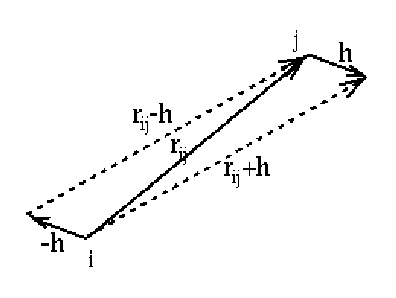
\epsfig{file=Implementation/vector_variation.eps, height=4cm}
  \caption{Addition of a vector at j equals the subtraction of the
  same vector at i}
  \label{vector_variation}
\end{center}
\end{figure}

As be can seen from figure \ref{vector_variation}\footnote{This is
  also easy to see from the relation $r_{ij} = \sqrt{
    \sum_{k=0}^{\bar{d}}(\xi_i^k-\xi_j^k)^2}$, 
where d is the number of dimensions, and $\bar{d}=d-1$.}, 

\begin{equation}
  r_{ij}(\xi_j+h) = r_{ij}(\xi_i-h)
\end{equation}

One object of class \emph{Distance} and 2d objects of class
\emph{DistanceDiff} holds all the information needed of the
inter-electronic distances for numerical calculation of both the
(centered difference) derivative and second derivative. Movement of
one electron consists of $(2d+1)\dot(N-1)$ updates of the distances,
and is thus of order ${\cal O}(N)$. Table \ref{Distance} give a list of the
public algorithms for the classes \emph{Distance} and
\emph{DistanceDiff}.

\begin{table}[hbtp]
\begin{center} {\large \bf Distance and DistanceDiff} \\ 
$\phantom{a}$ \\
\begin{tabular}{ll}
\hline\\ 
{\bf Algorithm}              & {\bf Usage} \\
Distance() or DistanceDiff() &Constructor\\
void attach(...)             &Attach intrinsic properties\\
void initialize()            &Initialize distances\\
void updateProposedMove()    &Calculate new distances for proposed move\\
void acceptMove()            &Accept proposed move\\
void rejectMove()            &Reject proposed move\\
double* getMatrix()          &Returns pointer to $rij$\\
double* getNewColumn()       &Returns pointer to $rij\_new\_column$\\
\hline
\end{tabular} 
\end{center}
\caption{Public algorithms for the classes Distance and DistanceDiff}
\label{Distance}
\end{table}

The differential parameters of
\emph{DistanceDiff}, $h$ and \emph{differentiate}, are assigned to
\emph{DistanceDiff} through the \emph{attach} algorithm. The value $h$
is the value added, or subtracted, to coordinate $differentiate$ of the
trial coordinate. \newline
An example on how to deal with upper triangular matrixes 
is in order. In the \emph{acceptMove} algorithm the new distances of
\emph{rij\_new\_column} is to be put into the upper-triangular matrix
$rij$. Here followes the \emph{acceptMove} algorithm:

{\footnotesize
\begin{enumerate}
\item[]
\begin{verbatim}
void Distance::acceptMove()
{
  __rij = rij-1+currentParticle;
  __rij_new_column = rij_new_column-1;
  int k=numParticles-1;
  for ( int i=0; i<currentParticle; i++ ) {
    (*__rij) = (*++__rij_new_column);
    k--;
    __rij+=k;
  }
  for ( int i=currentParticle+1; i<numParticles; i++)  
    (*++__rij)=(*++__rij_new_column);
  nextParticle();
}
\end{verbatim}

\end{enumerate}
}

For short we set $C=currentParticle$.
The pointer $\_\_rij$ is set to point at $r_{0C}$, if $C\ne
0$\footnote{If $C=0$ $\_\_rij$ is set to point at the element prior
  to the first element of $rij$},  
and $\_\_rij\_new\_column$ is set to point at the element
prior to the first element of $rij\_new\_column$\footnote{We
  create an extra element for this specific purpose.}.
Then we loop $i=0,C-1$, and set the value of $\_\_rij$ equal to the value
of the incremented $\_\_rij\_new\_column$, i.e. $r_{0C}$. We proceed
until $r_{\bar{C}C}$ (where $\bar{C}=C-1$). The pointer
$\_\_rij$ now points at $r_{\bar{C}\bar{N}}$, and in the
second loop it is incremented to point at $r_{CC^{^+}}$ (where $C^{^+}=C+1$),
and so is $\_\_rij\_new\_column$. Both pointers are incremented until
all the values are set, and we finally jump to the next particle.
\newline
Let us give an example of the $\_\_rij\_new\_column$ pointer. For $N=5$
and $C=2$ we have

\begin{equation}
  \begin{array}{cccccc}
  rij =
  |r_{01}, &r_{02}, \phantom{A} r_{03}, \phantom{A} r_{04}, &r_{12},
  \phantom{A} r_{13}, &r_{14}, &r_{23},
  &r_{24}, \phantom{A} r_{34}> \\
  pointer& \Uparrow \phantom{AAAAAAA}& \Uparrow \phantom{AAA}& \uparrow &
  \Uparrow & \Uparrow \phantom{AAAA}\\
  k& \phantom{AAA}3 & \phantom{AAAA}2 & \phantom{aa}1 & \phantom{aa}1 & 
  \end{array}
  \label{r_ij_array}
\end{equation}

We assign values at $\Uparrow$, and the $\uparrow$ is a temporary
pointer between the two loops.
This can more readily be seen by
looking at the corresponding matrix.

\begin{equation}
  r_{ij} = \left[
  \begin{array}{ccccc}
    0 & r_{01} & r_{02} & r_{03}  & r_{04}\\
    0 &   0    & r_{12} & r_{13}  & r_{14}\\
    0 &   0    &   0    & r_{23}  & r_{24}\\
    0 &   0    &   0    &   0     & r_{34}\\
    0 &   0    &   0    &   0     &   0   \\
  \end{array} \right]
\end{equation}

In the first loop we add one less than the number of none-zero
elements in the row we are at. Disregarding the none-zero elements,
this will take us to the element of the next row, with the same last index
(unless we are at the first element, in which case it will take us
to the last element).





%%%%%%%%%%%%%%%%%%%%% Jastrow and JastrowDiff %%%%%%%%%%%%%%%%%%%%
\subsection{Jastrow and JastrowDiff}

The classes \emph{Jastrow} and \emph{JastrowDiff} are similar to
\emph{Distance} and \emph{DistanceDiff}, respectively. First, they
contain information about the $f_{ij}$, in $f\_matrix$ (and the new
values for a proposed move, in \emph{f\_new\_column}). 
Furthermore, \emph{Jastrow} contains information about
the \emph{jastrowian}, $J$, and $\Delta J=J_{new}-J_{old}$.
Updating the $f_{ij}$'s for the jastrowian and its first and second
derivatives is also of order ${cal O}(N)$ (for the movement of one
electron).
Table \ref{Jastrow} lists the public algorithms of \emph{Jastrow} and
\emph{JastrowDiff}.

\begin{table}[hbtp]
\begin{center} {\large \bf Jastrow and JastrowDiff} \\ 
$\phantom{a}$ \\
\begin{tabular}{ll}
\hline\\ 
{\bf Algorithm}                        & {\bf Usage} \\
Jastrow() or JastrowDiff()             &  Constructor\\
void attach(...)                       &  Attach intrinsic properties\\
void initialize()                      &  Initialize the $f_{ij}$'s (and the jastrowian)\\
void updateProposedMove()              &Calculate new $f_{ij}$'s for proposed move\\
void acceptMove()                      &Accept proposed move\\
void rejectMove()                      &Reject proposed move\\
double* getFMatrix()                   &Returns pointer to $f\_matrix$\\
double* getFNewColumn()                &Returns pointer to $f\_new\_column$\\
void getFColumn(int i, double* fColumn)&Returns column i of $f\_matrix$ in fColumn\\
{\bf Jastrow-specific algorithms}      &\\
double\& operator()()                  &Returns the jastrowian, $J$\\
double getDifference()                 &Returns the difference, $\Delta J=J_{new}-J_{old}$\\
\hline
\end{tabular} 
 \end{center}
  \caption{Public algorithms for the classes Jastrow and JastrowDiff}
\label{Jastrow}
\end{table}

For example \emph{getFNewColumn} returns a pointer to:

\begin{equation}
  f\_new\_column = | f_{0i}, f_{1i}, \dots, f_{\bar{i}i}, f_{ii^{^+}},
  \dots, f_{i \bar{N}} >
\end{equation}

where $i$ is the current particle being moved.





%%%%%%%%%%%%%%%%%%%%% Derivatives %%%%%%%%%%%%%%%%%%%%
\subsection{Derivatives}

\emph{Derivatives} manages the derivatives of the $f_{ij}$'s. 
\newline
It is sufficient to calculate either $\frac{\delta f_{ij}}{\delta
  \xi_i}$ or $\frac{\delta f_{ij}}{\delta \xi_j}$, since 

\begin{equation}
  \frac{\delta f_{ij}}{\delta \xi_i} = \frac{\delta r_{ij}}{\delta \xi_i}
  \frac{d f_{ij}} {d r_{ij}} = - \frac{\delta r_{ij}}{\delta \xi_j}
  \frac{d f_{ij}} {d r_{ij}} = - \frac{\delta f_{ij}}{\delta \xi_j}
\end{equation}

In the above calculation we have used

\begin{equation}
  \frac{\delta r_{ij}}{\delta \xi_i^m} = \frac{\delta}{\delta \xi_i^m} 
  \sqrt{ \sum_{k=0}^{\bar{d}} (\xi_i^k-\xi_j^k)^2} =
  \frac{\xi_i^m-\xi_j^m}{r_{ij}} = - \frac{\delta
  r_{ij}}{\delta \xi_j^m} 
\end{equation}

where $\xi_i^m$ is cordinate $m$ of particle $i$, and $\bar{d}=d-1$. \newline
The upper triangular matrix:

\begin{equation}
  \frac{\delta f}{\delta \xi} = \left[
  \begin{array}{ccccc}
    0 & \frac{\delta f_{01}}{\delta \xi_1} & \frac{\delta
    f_{02}}{\delta \xi_2} & \dots & \frac{\delta f_{0\bar{N}}}{\delta
    \xi_{\bar{N}}} \\ 
    0 &        0        & \frac{\delta f_{12}}{\delta \xi_2} & \dots & 
    \frac{\delta f_{1\bar{N}}}{\delta \xi_{\bar{N}}} \\
    0 &        0        &          0            &\ddots &  \vdots       \\
    0 &        0        &          0            &   0   &
    \frac{\delta f_{\bar{\bar{N}}\bar{N}}}{\delta \xi_{\bar{N}}} \\
    0 &        0        &          0            &   0   &   0  
  \end{array} \right]
\label{df_dxi}
\end{equation}

is stored as an array, \emph{derivatives}, similar to that of
eq. (\ref{r_ij_array}). Also, we store 
the upper-triangular matrix of the second derivatives. The calculation
of the first derivative,

\begin{equation}
  \frac{\delta f_{ij}}{\delta \xi_i} \approx \frac{f_{ij}(\xi_i+h) -
  f_{ij}(\xi_i-h)}{2h} 
\end{equation}

and the second derivative,

\begin{equation}
  \frac{\delta^2 f_{ij}}{\delta \xi_i^2} \approx \frac{f_{ij}(\xi_i+h)
  + f_{ij}(\xi_i-h) - 2 f_{ij}}{h^2}
\end{equation}

uses the $f_{ij}$'s updated in \emph{Jastrow} and
\emph{JastrowDiff}. Movement of one particle involves
calculation of $N-1$ values of both $\frac{\delta f_{ij}}{\delta \xi_i}$
and $\frac{\delta^2 f_{ij}}{\delta \xi_i^2}$. Table \ref{Derivatives}
lists the public algorithms of \emph{Derivatives}.

\begin{table}[hbtp]
\begin{center} {\large \bf Derivatives} \\ 
$\phantom{a}$ \\
\begin{tabular}{ll}
\hline\\ 
{\bf Algorithm}                   & {\bf Usage} \\
Derivatives()                     &Constructor\\
void attach(...)                  &Attach intrinsic properties\\
void initialize()                 &Initialize the derivatives\\
void updateDerivatives()          &Calculate the new derivatives for a move\\ 
void acceptDerivatives()          &Updates the 1. and 2. derivatives matrix\\
void rejectDerivatives()          &Jumps to next particle without doing
anything\\
void getDColumn(int i, double* Column) 
  &Returns column i of $\frac{\delta f}{\delta \xi}$ in Column\\
double* getDNewColumn() &Returns pointer to new derivatives\\
void getD2Column(int i, double* Column)
  &Returns column i of $\frac{\delta^2 f}{\delta \xi^2}$ in Column\\
double* getD2NewColumn()&Returns pointer to new second derivatives\\
\hline
\end{tabular} 
 \end{center}
  \caption{Public algorithms for the class Derivatives}
\label{Derivatives}
\end{table}



%%%%%%%%%%%%%%%%%%%%% Correlation %%%%%%%%%%%%%%%%%%%%
\subsection{Correlation}

Before we proceed with the class structure, some theory must be
established. Let us start with the ratio
$\frac{G_{new}}{G_{old}}$, for the Metropolis algorithm. For $G=J$ we
have 

\begin{equation}
  \frac{G_{new}}{G_{old}} = \frac{J_{old}+\Delta J}{J_{old}}
\end{equation}

and for $G=e^J$,

\begin{equation}
  \frac{G_{new}}{G_{old}} = e^{\Delta J}
\end{equation}

$\nabla^2 J$ given by, 

\begin{equation}
  \nabla^2 J = \sum_{i=0}^{\bar{N}} \nabla_i^2 J =
  \sum_{i=0}^{\bar{N}} \nabla_i^2 \sum_{k<l} f_{kl} = 
  \sum_{i=0}^{\bar{N}} \left[ \sum_{k<l} \delta_{li} \nabla_i^2 f_{kl}
  + \sum_{k<l} \delta_{ki} \nabla_i^2 f_{kl} \right]
\end{equation}

where $\nabla_i^2 f_{ij} = \sum_{k=0}^{\bar{d}} \frac{\delta^2
  f_{ij}}{(\delta \xi_i^k)^2}$, and $\delta_{li}$ is the
Kronecker-delta. We define

\begin{equation}
  \nabla_i^2 J \equiv \sum_{j=0}^{i-1} \nabla_i^2 f_{ij}  +
  \sum_{j=i+1}^{\bar{N}} \nabla_j^2 f_{ij}
\end{equation}

and get 

\begin{equation}
  \nabla^2 J = \sum_{i=0}^{\bar{N}} \left[ \sum_{j=0}^{i-1} \nabla_i^2 f_{ij}
  + \sum_{j=i+1}^{\bar{N}} \nabla_i^2 f_{ij} \right] =
  \sum_{i=0}^{\bar{N}} \nabla_i^2 J
\end{equation}

from the relation $\nabla_i^2 f_{ij} = \nabla_j^2 f_{ij}$. If we move
one particle, $C$, all values in $\nabla^2_C J$, and one of the values
in $\nabla^2_i J$, $i\ne C$, are changed;

\begin{equation}
  \nabla_i^2 J^{new} = \nabla_i^2 J^{old} + \nabla_i^2 f_{iC}^{new} - \nabla_i^2 f_{iC}^{old}
\end{equation}

for all $i\ne C$, and

\begin{equation}
  \nabla_C^2 J^{new} = \sum_{i \ne C} \nabla_i^2 f_{iC}^{new}
\end{equation}

By changing only these values, we have an algorithm of order ${\cal O}(N)$
for the update of $\nabla^2 J$. \newline
For $\nabla J$, we have

\begin{equation}
  \nabla J = \left| \frac{\delta J}{\delta \xi_0^0},
  \dots , \frac{\delta J}{\delta \xi_{\bar{d}}^0}, \dots,
  \frac{\delta J}{\delta \xi_0^{\bar{N}}}, \dots, \frac{\delta J}{\delta
  \xi_{\bar{d}}^{\bar{N}}} \right>
\end{equation}

where

\begin{equation}
  \frac{\delta J}{\delta \xi^i} = \frac{\delta}{\delta \xi^i}
  \sum_{k<l} f_{kl} = \sum_{j=0}^{i-1} \frac{\delta f_{ji}}{\delta
  \xi^i}  + \sum_{j=i+1}^{\bar{N}} \frac{\delta f_{ij}}{\delta \xi^i} 
  = \sum_{j=0}^{i-1} \frac{\delta f_{ji}}{\delta
  \xi^i}  - \sum_{j=i+1}^{\bar{N}} \frac{\delta f_{ij}}{\delta \xi^j}
\end{equation}

since $\frac{\delta f_{ij}}{\delta \xi^i} = - \frac{\delta
  f_{ij}}{\delta \xi^j}$. 
All the values of the derivatives are kept
in the $d$ objects of class \emph{Derivatives}, and its easy to
calculate the above expression. However, we wish to keep the order of
our correlation routines as low as possible, so we follow a procedure
similar to that of $\nabla^2 J$;

\begin{equation}
  \frac{\delta J^{new}}{\delta \xi^i} = \frac{\delta J^{old}}{\delta
  \xi^i} + \frac{\delta f_{ji}^{new}}{\delta \xi^i} - \frac{\delta
  f_{ji}^{old}}{\delta \xi^i} 
\end{equation} 

for $i<C$,

\begin{equation}
  \frac{\delta J^{new}}{\delta \xi^i} = \frac{\delta J^{old}}{\delta
  \xi^i} - \frac{\delta f_{ji}^{new}}{\delta \xi^j} + \frac{\delta
  f_{ji}^{old}}{\delta \xi^j} 
\end{equation} 

for $i>C$, and for $C$

\begin{equation}
  \frac{\delta J^{new}}{\delta \xi^C} 
  = \sum_{j=0}^{C-1} \frac{\delta f_{jC}^{new}}{\delta
  \xi^C}  - \sum_{j=C+1}^{\bar{N}} \frac{\delta f_{Cj}^{new}}{\delta \xi^j}
\end{equation}

For $G=J$ we can use the above relations directly. For $G=e^J$ a few
minor modifications must be made:

\begin{equation}
  \nabla e^J = \nabla J \dot e^J
\end{equation}

and

\begin{equation}
  \nabla^2 e^J = \nabla (\nabla J \dot e^J) = \left[ \nabla^2 J +
  (\nabla J)^2  \right] e^J
\end{equation}

I.e. $e^J$, $\nabla J$ and $\nabla^2 J$ holds all the information needed to
compute $\nabla e^J$ and $\nabla^2 e^J$. The above computations are
also of the order ${\cal O}(N)$. \newline


\emph{Correlation} is the class used by the VMC-algorithm to manage
all information 
about the correlation. It is used to calculate the gradient, and the
gradient squared, of the correlation. Also, the ratio
$\frac{G_{new}}{G_{old}}$ for a proposed move is calculated, as well
as the value of the correlation, $G$, itself. Routines for both
thermalization- and VMC-moves are implemented. \newline
Table \ref{Correlation} lists the public algorithms of \emph{Correlation}.

\begin{table}[hbtp]
\begin{center} {\large \bf Correlation} \\ 
$\phantom{a}$ \\
\begin{tabular}{ll}
\hline\\ 
{\bf Algorithm}                 & {\bf Usage} \\
Derivatives(Domain\& domain)    &Constructor\\
void proposeMove()              &Updates the values (in the Jastrow and
Distance objects)\\
 & needed to determine the ratio $\frac{G_{new}}{G_{old}}$\\
void initializeThermalizedMove()&Initializes the Jastrow and Distance objects\\
void acceptThermalizedMove()    &Updates the Jastrow and Distance objects\\
void rejectThermalizedMove()    &Jumps to next particle without doing anything\\
void initializeVMC()            &Initializes the JastrowDiff, DistanceDiff 
              and Derivatives\\ 
&objects, and initializes $\nabla G$ and $\nabla^2 G$\\
void acceptVMCMove()            &Update $\nabla G$ and $\nabla^2 G$,
and updates the Jastrow, JastrowDiff,\\
& Distance, DistanceDiff and Derivatives objects\\
void rejectVMCMove()            &Jumps to next particle without doing anything\\
double operator()()             &Returns the correlation, $G$,
i.e. either $J$ or $e^J$\\
double getRatio()               &Returns the ratio $\frac{G_{new}}{G_{old}}$\\
double* getGradient()           &Returns pointer to $\nabla G$\\
double getGrad2()               &Returns the value of $\nabla^2 G$\\
\hline
\end{tabular} 
 \end{center}
  \caption{Public algorithms for the class Correlation}
\label{Correlation}
\end{table}

The constructor uses the \emph{Domain} class to access information
about properties like the number of particles $N$, the number of
dimensions $d$, and all the coordinates. The \emph{proposeMove}
algorithm updates the changes in the jastrowian due to a proposed move
in the trial coordinate. Furthermore, it stores the
new inter-electronic distances, and the new $f_{ij}$'s in two arrays;
\emph{rij\_new\_column} in the object of class\emph{Distance} and
\emph{f\_new\_column} in the object of class \emph{Jastrow}. \newline 
If the move is accepted, the values of the differences must be
updated, as well as the derivatives and the gradients (for a VMC
move\footnote{In the case of thermalization, no
  sample of the energy is preformed, so no derivatives (or
  differences) are calculated.}). 
In the \emph{acceptVMCmove} algorithm, see table \ref{Correlation}, the
values of $\nabla J$ and $\nabla^2 J$ are calculated. $\nabla G$
and $\nabla^2 G$ are not calculated until the \emph{getGradient} and
\emph{getGrad2} routines.
Finally, all new values must be assigned to their respective
upper-triangular matrices, before we proceed to the next particle. 
\newline
If the move is not accepted, we simply proceed to the next particle,
without performing any changes.



%%%%%%%%%%%%%%%%%%%%% CoorExt %%%%%%%%%%%%%%%%%%%%
\subsection{CoorExt}

The class \emph{CoorExt}, defined in \emph{Coor.h}, manages the
particles coordinates. Table 
\ref{CoorExt} lists the public algorithms of \emph{CoorExt}. 

\begin{table}[hbtp]
\begin{center} {\large \bf CoorExt} \\ 
$\phantom{a}$ \\
\begin{tabular}{ll}
\hline\\ 
{\bf Algorithm}                   & {\bf Usage} \\
CoorExt()                         & Empty constructor\\
CoorExt(double* x, int \_len,     & Constructor\\
\phantom{a} int \_\_spin, double* \_ext)& \\
void attach(double* \_\_x, int \_len,& Attaches intrinsic properties\\
\phantom{a} int \_\_spin, double* \_ext)& \\
double\& operator()()             & Returns the current cartesian coordinate\\
double\& operator()(int num)      & Returns coordinate num\\
void operator++(int)              & Increments pointer to next cartesian coordinate\\
void resetPtr                     & Resets pointer to first cartesian coordinate\\
int getLen()                      & Returns the number of cartesian coordinates\\
double r()                        & Returns the distance form the nucleus\\
void calculateR()                 & Computes the distance to the nucleus\\
int\& spin()                      & Returns the electron eigen-spin\\
int flipSpin()                    & Returns negative multiple of spin\\
double param(int i)               & Returns the value of parmeter number i; ext[i]\\
\hline
\end{tabular} 
 \end{center}
  \caption{Public algorithms for the class CoorExt}
\label{CoorExt}
\end{table}

\emph{CoorExt} contains all the information needed of each electron;
its cartesian coordinates and its eigen-spin. Furthermore, it contains
a pointer to the variational parameters of the Slater determinant
orbital wave-functions. In this manner one orbital function may be
computed directly given one \emph{CoorExt} object.
Also, the electron distance from the origin is calculated, and it
allows a spin flip.



%%%%%%%%%%%%%%%%%%%%% FuncSetMultivar %%%%%%%%%%%%%%%%%%%%
\subsection{FuncSetMultivar}

The class \emph{FuncSetMultivar}, defined in \emph{Func.h}, manages a
set of functions and their 
derivatives. Each column in a Slater matrix is represented as one such
object. Table \ref{FuncSetMultivar} lists some\footnote{All the
  \emph{attach} procedures are left out, Furthermore, most of the
  algorithms are implemented twice; ($\dots$) means either with or
  without an input (\emph{Param\& \_coordinate}).} of the public algorithms
of \emph{FuncSetMultivar}.

\begin{table}[hbtp]
\begin{center} {\large \bf FuncSetMultivar} \\ 
$\phantom{a}$ \\
\begin{tabular}{ll}
\hline\\ 
{\bf Algorithm}                   & {\bf Usage} \\
FuncSetMultivar($\dots$)          & Constructor\\
void init($\dots$)                & Initialize intrinsic properties\\
void calcValueCenter($\dots$)     & Calculates the function values (given coordinate)\\
void calcValueSides($\dots$)      & Calculates the function values (given differentiated coordinate)\\

double valuePt()                  & Returns pointer to different calculated values\\
double diff()                     & Calculates the first derivatives\\
double diff(int v)                & Calculates the first derivatives
with respect to the\\
                                  & indexed variable (of all functions)\\
double ddiff()                    & Calculates the second derivatives\\
\hline
\end{tabular} 
 \end{center}
  \caption{Public algorithms for the class FuncSetMultivar}
\label{FuncSetMultivar}
\end{table}

In order to find the derivatives of the functions for a given
coordinate, \emph{calcValueCenter} and \emph{calcValueSides}
must be called prior to \emph{diff}. The second derivatives are
calculated with a call to the \emph{ddiff} algorithm.



%%%%%%%%%%%%%%%%%%%%% Functor %%%%%%%%%%%%%%%%%%%%
\subsection{Functor}

The template class \emph{Functor} defines a functor. 
We have chosen to use a functor-type object, to increase
flexibility, and have the ability to use more complex functions
later without changing too much code\footnote{This is good programming
  philosophy; we may want to improve the program at a later stage.}.
Table \ref{Functor} lists the public algorithm of \emph{Functor}.

\begin{table}[hbtp]
\begin{center} {\large \bf Functor} \\ 
$\phantom{a}$ \\
\begin{tabular}{ll}
\hline\\ 
{\bf Algorithm}                   & {\bf Usage} \\
Functor()                         & Empty constructor\\
Functor(Function\& \_function)    & Constructor\\
void attach(Function\& \_function)& Attaches a function\\
Return operator()(Param\& coor)   & Returns an object of type Return\\
\hline
\end{tabular} 
 \end{center}
  \caption{Public algorithms for the class Functor}
\label{Functor}
\end{table}


Given an argument 
\emph{Param} the functor returns \emph{Return}. Both \emph{Param} and
\emph{Return} are classes, e.g. \emph{double}, \emph{CoorExt} etc.
To give an example, we can create a functor with the call:

{\footnotesize
\begin{enumerate}
\item[]
  \begin{verbatim}
Functor<CoorExt, double>* function;
function = new Functor<CoorExt, double>();
\end{verbatim}

\end{enumerate}
}

We need some formula for calculating the return value of type
\emph{double}, given an object of class \emph{CoorExt}. If we first
define the function \emph{hydr1s} given by:

{\footnotesize
\begin{enumerate}
\item[]
  \begin{verbatim}
double hydr1s(CoorExt& coordinate) {
  return exp(- coordinate.param(0) * coordinate.r());
}
\end{verbatim}

\end{enumerate}
}

and then attach it to the \emph{Functor} object \emph{function}:

{\footnotesize
\begin{enumerate}
\item[]
  \begin{verbatim}
function[0].attach(hydr1s);
\end{verbatim}

\end{enumerate}
}

We may then calculate the value of the function with the call:

{\footnotesize
\begin{enumerate}
\item[]
  \begin{verbatim}
function_value = (function[0])(coordinate);
\end{verbatim}

\end{enumerate}
}

where \emph{coordinate} is an object of class \emph{CoorExt}. 



%%%%%%%%%%%%%%%%%%%%% Random %%%%%%%%%%%%%%%%%%%%
\subsection{Random}

The two classes \emph{Ran0} and \emph{Ran1}, in
\emph{Random.h}, defines the random generators used by the
Metropolis random movement. We want our electrons to move \emph{randomly}
in space, and at the same time we want to reduce the CPU-time of our
calculations. Therefore, the program should be tested with different
random generators. Table \ref{Random} lists the
public algorithms of the random generators.

\begin{table}[hbtp]
\begin{center} {\large \bf Random} \\ 
$\phantom{a}$ \\
\begin{tabular}{ll}
\hline\\ 
{\bf Algorithm}                   & {\bf Usage} \\
Ran0(long seed) or Ran1(long seed)& Constructor\\
double getNum(void)               & Returns double in the range (0,1]\\
\hline
\end{tabular} 
 \end{center}
  \caption{Public algorithms for the class Random}
\label{Random}
\end{table}

We will not get into the details of the random generators, and simply
refere to \emph{???reference here???}. However, of importance to the
user is the integral seed. This seed is changed with each call to
\emph{getNum}. Giving the same seed twice produces the exact same
number, and if called several times they will produce the same
sequences of numbers. To produce indepentent runs, the seed
must differ with each run\footnote{An other problem may also
  arise. Even with two different seeds, one of the sequences may by
  chance produce the other seed, and thereby produce the same sequence
following this number. This problem will not be addressed in this
scope, but note that this chance is extremely small, and given two
different starting positions, the Metropolis algorithm should not
become too biased even if this were to occur.}










































